\documentclass[12pt,twoside,a4paper]{report}
\usepackage{etex}
% Select encoding of your inputs.
\usepackage[utf8]{inputenc}

% Make latex understand and use the typographic
% rules of the language used in the document.
\usepackage[english, danish]{babel}

% Use the vector font Latin Modern which is going
% to be the default font in latex in the future.
\usepackage{lmodern}

% Choose the font encoding
\usepackage[T1]{fontenc}

% Use colour in tables
\usepackage[table]{xcolor}
\usepackage{array}
\usepackage{multirow}

% load a colour package
\usepackage{xcolor}
\definecolor{aaublue}{RGB}{33,26,82}% dark blue

% The standard graphics inclusion package
\definecolor{white}{RGB}{255,255,255} % define color white
\usepackage{graphicx}
\usepackage{adjustbox}

% Set up how figure and table captions are displayed
\usepackage{caption}
\captionsetup{
  font=footnotesize,% set font size to footnotesize
  labelfont=bf % bold label (e.g., Figure 3.2) font
}

% Enable row combination in tables
\usepackage{multirow}

% Make space between table lines and text
\renewcommand{\arraystretch}{1.5}

% Make the standard latex tables look so much better
\usepackage{array,booktabs}

% Enable the use of frames around, e.g., theorems
% The framed package is used in the example environment
\usepackage{framed}
\usepackage{colortbl}
\usepackage{longtable}
\usepackage{xcolor}
\usepackage{textcomp}

%%%%%%%%%%%%%%%%%%%%%%%%%%%%%%%%%%%%%%%%%%%%%%%%
% Mathematics
%%%%%%%%%%%%%%%%%%%%%%%%%%%%%%%%%%%%%%%%%%%%%%%%
% Defines new environments such as equation,
% align and split 
\usepackage{amsmath}
\usepackage{relsize}
% Adds new math symbols
\usepackage{amssymb}
% Use theorems in your document
% The ntheorem package is also used for the example environment
% When using thmmarks, amsmath must be an option as well. Otherwise \eqref doesn't work anymore.
\usepackage[framed,amsmath,thmmarks]{ntheorem}
\usepackage{cancel}

%%%%%%%%%%%%%%%%%%%%%%%%%%%%%%%%%%%%%%%%%%%%%%%%
% Page Layout
%%%%%%%%%%%%%%%%%%%%%%%%%%%%%%%%%%%%%%%%%%%%%%%%
% Change margins, papersize, etc of the document
\usepackage[
  left=25mm,% left margin on an odd page %tidligere 25mm for baade right og left
  right=25mm,% right margin on an odd page
  top=35mm,
  ]{geometry}
  
% Modify how \chapter, \section, etc. look
% The titlesec package is very configureable
\usepackage{titlesec}
\makeatletter
\def\ttl@mkchap@i#1#2#3#4#5#6#7{%
    \ttl@assign\@tempskipa#3\relax\beforetitleunit
    \vspace{\@tempskipa}%<<<<<< REMOVE THE * AFTER \vspace
    \global\@afterindenttrue
    \ifcase#5 \global\@afterindentfalse\fi
    \ttl@assign\@tempskipb#4\relax\aftertitleunit
    \ttl@topmode{\@tempskipb}{%
        \ttl@select{#6}{#1}{#2}{#7}}%
    \ttl@finmarks  % Outside the box!
    \@ifundefined{ttlp@#6}{}{\ttlp@write{#6}}}
\makeatother

\titlespacing{\chapter}{0pt}{0pt}{10pt}
\titlespacing{\section}{0pt}{0pt}{-5pt}
\titlespacing{\subsection}{0pt}{8pt}{-5pt}
\titlespacing{\subsubsection}{0pt}{6pt}{-10pt}

\titleformat*{\section}{\normalfont\Large\bfseries\color{aaublue}}
\titleformat*{\subsection}{\normalfont\large\bfseries\color{aaublue}}
\titleformat*{\subsubsection}{\normalfont\normalsize\bfseries\color{aaublue}}

\usepackage{bookmark}
\usepackage{titlesec, blindtext, color}
%\color{gray75}{gray}{0.75}
\newcommand{\hsp}{\hspace{20pt}}
\titleformat{\chapter}[hang]{\Huge\bfseries}{\thechapter\hsp\textcolor{aaublue}{|}\hsp}{0pt}{\Huge\bfseries}

% Change the headers and footers
\usepackage{fancyhdr}
\setlength{\headheight}{15pt}
\pagestyle{fancy}
\fancyhf{} %delete everything
\renewcommand{\headrulewidth}{0pt} %remove the horizontal line in the header
\fancyhead[RO,LE]{\color{aaublue}\small\nouppercase\leftmark} %even page - chapter title
\fancyhead[LO]{}
\fancyhead[RE]{} 
\fancyhead[CE]{}
\fancyhead[CO]{}
\fancyfoot[RE,LO]{\thepage}
\fancyfoot[LE,RO]{B205} %page number on all pages
\fancyfoot[CE,CO]{}

% change first page of all chapters header and footer to fancy style
\makeatletter
\let\ps@plain\ps@fancy
\makeatother

% Do not stretch the content of a page. Instead,
% insert white space at the bottom of the page
\raggedbottom

% Enable arithmetics with length. Useful when typesetting the layout.
\usepackage{calc}

%%%%%%%%%%%%%%%%%%%%%%%%%%%%%%%%%%%%%%%%%%%%%%%%
% Bibliography
%%%%%%%%%%%%%%%%%%%%%%%%%%%%%%%%%%%%%%%%%%%%%%%%
%setting references (using numbers) and supporting i.a. Chicargo-style:
\usepackage{etex}
\usepackage{etoolbox}
\usepackage{keyval}
\usepackage{ifthen}
\usepackage{url}
\usepackage{csquotes}
\usepackage[backend=biber, url=true, doi=true, style=numeric, sorting=none]{biblatex}
\addbibresource{setup/bibliography.bib}

%%%%%%%%%%%%%%%%%%%%%%%%%%%%%%%%%%%%%%%%%%%%%%%%
% Misc
%%%%%%%%%%%%%%%%%%%%%%%%%%%%%%%%%%%%%%%%%%%%%%%%

%%% Enables the use FiXme refferences. Syntax: \fxnote{...} %%%
\usepackage[footnote, draft, english, silent, nomargin]{fixme}
%With "final" instead of "draft" an error will ocure for every FiXme under compilation.

%%% allows use of lorem ipsum (generate i.e. pagagraph 1 to 5 with \lipsum[1-5]) %%%
\usepackage{lipsum}

%%% Enables figures with text wrapped tightly around it %%%
\usepackage{wrapfig}

%%% Section debth included in table of contents (1 = down to sections) %%%
\setcounter{tocdepth}{1}

%%% Section debth for numbers (1 = down to sections) %%%
\setcounter{secnumdepth}{1}

\usepackage{tocloft}
\setlength{\cftbeforetoctitleskip}{0 cm}
\renewcommand{\cftpartpresnum}{Part~}
\let\cftoldpartfont\cftpartfont
\renewcommand{\cftpartfont}{\cftoldpartfont\cftpartpresnum}

%%%%%%%%%%%%%%%%%%%%%%%%%%%%%%%%%%%%%%%%%%%%%%%%
% Hyperlinks
%%%%%%%%%%%%%%%%%%%%%%%%%%%%%%%%%%%%%%%%%%%%%%%%

% Enable hyperlinks and insert info into the pdf
% file. Hypperref should be loaded as one of the 
% last packages
\usepackage{nameref}
\usepackage{hyperref}
\hypersetup{%
	%pdfpagelabels=true,%
	plainpages=false,%
	pdfauthor={Author(s)},%
	pdftitle={Title},%
	pdfsubject={Subject},%
	bookmarksnumbered=true,%
	colorlinks,%
	citecolor=aaublue,%
	filecolor=aaublue,%
	linkcolor=aaublue,% you should probably change this to black before printing
	urlcolor=aaublue,%
	pdfstartview=FitH%
}

% remove all indentations
\setlength\parindent{0pt}
\parskip 5mm
\usepackage{verbatim}

\definecolor{Gra}{RGB}{230,230,230}

%creates a nice-looking C#-text
\newcommand{\CC}{C\nolinebreak\hspace{-.05em}\raisebox{.3ex}{\scriptsize\text \#} }

%enables multi column lists
\usepackage{multicol}

%enables code-examples
\usepackage{listings}

\definecolor{coolblue}{RGB}{32,95,128}
\definecolor{mygreen}{rgb}{0,0.6,0}
\definecolor{mygray}{rgb}{0.5,0.5,0.5}
\definecolor{mymauve}{rgb}{0.58,0,0.82}
\usepackage{textcomp}
\definecolor{listinggray}{gray}{0.9}
\definecolor{lbcolor}{rgb}{0.9,0.9,0.9}

\lstset{
%  backgroundcolor=\color{white},   % choose the background color; you must add \usepackage{color} or \usepackage{xcolor}
%  basicstyle=\footnotesize,        % the size of the fonts that are used for the code
%  breakatwhitespace=false,         % sets if automatic breaks should only happen at whitespace
%  breaklines=true,                 % sets automatic line breaking
%  captionpos=t,                    % sets the caption-position to bottom
%  commentstyle=\color{mygreen},    % comment style
%  deletekeywords={...},            % if you want to delete keywords from the given language
%  escapeinside={\%*}{*)},          % if you want to add LaTeX within your code
%  extendedchars=true,              % lets you use non-ASCII characters; for 8-bits encodings only, does not work with UTF-8
%  frame=single,                    % adds a frame around the code
%  keepspaces=true,                 % keeps spaces in text, useful for keeping indentation of code (possibly needs columns=flexible)
%  keywordstyle=\color{blue},       % keyword style
%  language=C++,                 % the language of the code
%  morekeywords={*,...},            % if you want to add more keywords to the set
%  numbers=left,                    % where to put the line-numbers; possible values are (none, left, right)
%  numbersep=5pt,                   % how far the line-numbers are from the code
%  numberstyle=\tiny\color{mygray}, % the style that is used for the line-numbers
%  rulecolor=\color{black},         % if not set, the frame-color may be changed on line-breaks within not-black text (e.g. comments (green here))
%  showspaces=false,                % show spaces everywhere adding particular underscores; it overrides 'showstringspaces'
%  showstringspaces=false,          % underline spaces within strings only
%  showtabs=false,                  % show tabs within strings adding particular underscores
%  stepnumber=1,                    % the step between two line-numbers. If it's 1, each line will be numbered
%  stringstyle=\color{mymauve},     % string literal style
%  tabsize=2,                       % sets default tabsize to 2 spaces
%  title=\lstname                   % show the filename of files included with \lstinputlisting; also try caption instead of title
backgroundcolor=\color{lbcolor},
	tabsize=4,
	rulecolor=,
	language=C,
        basicstyle=\scriptsize,
        upquote=true,
        aboveskip={1.5\baselineskip},
        columns=fixed,
        showstringspaces=false,
        extendedchars=true,
        breaklines=true,
        prebreak = \raisebox{0ex}[0ex][0ex]{\ensuremath{\hookleftarrow}},
        frame=single,
        showtabs=false,
        numbers=left,
        captionpos=b,
        numbersep=5pt,
        numberstyle=\tiny\color{mygray},
        showspaces=false,
        showstringspaces=false,
        identifierstyle=\ttfamily,
        keywordstyle=\color[rgb]{0,0,1},
        commentstyle=\color[rgb]{0.133,0.545,0.133},
        stringstyle=\color[rgb]{0.627,0.126,0.941},
}

\usepackage{float}
\usepackage{caption}
\usepackage{subcaption}
\usepackage{siunitx}
\sisetup{decimalsymbol=comma}
\sisetup{detect-weight}

\usepackage{enumitem}
%\usepackage[citestyle=authoryear,natbib=true]{biblatex}

% Figures - TIKZ
\usepackage{tikz}
\usetikzlibrary{shapes,arrows}
\usepackage[americanresistors,americaninductors,americancurrents, americanvoltages]{circuitikz}

% Wall of text logo
\newcommand{\walloftextalert}[0]{\includegraphics[width=\textwidth]{walloftext.png}}

\usepackage{pdfpages}
\usepackage{lastpage}
\usepackage{epstopdf}

\setlength{\headheight}{21pt}

\hfuzz=\maxdimen
\tolerance = 10000
\hbadness  = 10000

\usepackage{siunitx}
\graphicspath{{./figures/}}% package inclusion and set up of the document

%%%%%%%%%%%%%%%%%%%%%%%%%%%%%%%%%%%%%%%%%%%%%%%%%%%%%
%             UNITS, EQUATIONS AND TEXT             %
%%%%%%%%%%%%%%%%%%%%%%%%%%%%%%%%%%%%%%%%%%%%%%%%%%%%%
%Units:
\newcommand{\unit}[1]{&& \left[\si{#1}\right]} %\newcommand{\unit}[1]{[\si{#1}]}             <<| Use these if you want equations to be
\newcommand{\unitWh}[1]{[\si{#1}]}             %\newcommand{\eq}[2]{&&\si{#1} &= \si{#2}&&}  <<| centered.. .. will appear scrambled
\newcommand{\numUnit}[1]{\ \si{#1}&}           %                                               | from one equation to the next though..
%Equation:                                     %                                               | and does not work with long equations.. :/
\newcommand{\eq}[2]{\si{#1} &= \si{#2}}
\newcommand{\arw}{&& &\Updownarrow&&}
%Text:
\newcommand{\tx}[1]{\text{#1}}
%Vectors
\renewcommand{\vec}[1]{\boldsymbol{\mathbf{#1}}}

%%%%%%%%%%%%%%%%%%%%%%%%%%%%%%%%%%%%%%%%%%%%%%%%%%%%%
%                  REFERENCES                       %
%%%%%%%%%%%%%%%%%%%%%%%%%%%%%%%%%%%%%%%%%%%%%%%%%%%%%

%Chapter
\newcommand{\Chapref}[1]{\emph{Chapter \ref{#1}}}
\newcommand{\chapref}[1]{\emph{chapter \ref{#1}}}
%Section
\newcommand{\Secref}[1]{\emph{Section \ref{#1}}}
\newcommand{\secref}[1]{\emph{section \ref{#1}}}
%subSection
\newcommand{\Subsecref}[1]{\emph{Subsection \ref{#1}}}
\newcommand{\subsecref}[1]{\emph{subsection \ref{#1}}}
%Appendix
\newcommand{\Appref}[1]{\emph{Appendix \ref{#1}}}
\newcommand{\appref}[1]{\emph{appendix \ref{#1}}}
%Listings
\newcommand{\Coderef}[1]{\emph{Listings: \ref{#1}}}
\newcommand{\coderef}[1]{\emph{listings: \ref{#1}}}
%Figure:
\newcommand{\Figref}[1]{\emph{Figure \ref{#1}}}
\newcommand{\figref}[1]{\emph{figure \ref{#1}}}
%Table:
\newcommand{\Tableref}[1]{\emph{Table \ref{#1}}}
\newcommand{\tableref}[1]{\emph{table \ref{#1}}}

%Expressions:
\newcommand{\Expr}[1]{\emph{Expression (\ref{#1})}}
\newcommand{\expr}[1]{\emph{expression (\ref{#1})}}

%Equations:
%1 equation:
\newcommand{\Eqref}[1]{\emph{Equation (\ref{#1})}}
\renewcommand{\eqref}[1]{\emph{equation (\ref{#1})}}
%2 equations:
\newcommand{\EqrefTwo}[2]{\emph{Equation (\ref{#1})} and \emph{(\ref{#2})}}
\newcommand{\eqrefTwo}[2]{\emph{equation (\ref{#1})} and \emph{(\ref{#2})}}
%3 equations:
\newcommand{\EqrefThree}[3]{\emph{Equation (\ref{#1})}, \emph{(\ref{#2})} and \emph{(\ref{#3})}}
\newcommand{\eqrefThree}[3]{\emph{equation (\ref{#1})}, \emph{(\ref{#2})} and \emph{(\ref{#3})}}
%4 equations:
\newcommand{\EqrefFour}[4]{\emph{Equation (\ref{#1})}, \emph{(\ref{#2})}, \emph{(\ref{#3})} and \emph{(\ref{#4})}}
\newcommand{\eqrefFour}[4]{\emph{equation (\ref{#1})}, \emph{(\ref{#2})}, \emph{(\ref{#3})} and \emph{(\ref{#4})}}
%5 equations:
\newcommand{\EqrefFive}[5]{\emph{Equation (\ref{#1})}, \emph{(\ref{#2})}, \emph{(\ref{#3})}, \emph{(\ref{#4})} and \emph{(\ref{#5})}}
\newcommand{\eqrefFive}[5]{\emph{equation (\ref{#1})}, \emph{(\ref{#2})}, \emph{(\ref{#3})}, \emph{(\ref{#4})} and \emph{(\ref{#5})}}
%6 equations:
\newcommand{\EqrefSix}[6]{\emph{Equation (\ref{#1})}, \emph{(\ref{#2})}, \emph{(\ref{#3})}, \emph{(\ref{#4})}, \emph{(\ref{#5})} and \emph{(\ref{#6})}}
\newcommand{\eqrefSix}[6]{\emph{equation (\ref{#1})}, \emph{(\ref{#2})}, \emph{(\ref{#3})}, \emph{(\ref{#4})}, \emph{(\ref{#5})} and \emph{(\ref{#6})}}
%7 equations:
\newcommand{\EqrefSeven}[7]{\emph{Equation (\ref{#1})}, \emph{(\ref{#2})}, \emph{(\ref{#3})}, \emph{(\ref{#4})}, \emph{(\ref{#5})}, \emph{(\ref{#6})} and \emph{(\ref{#7})}}
\newcommand{\eqrefSeven}[7]{\emph{equation (\ref{#1})}, \emph{(\ref{#2})}, \emph{(\ref{#3})}, \emph{(\ref{#4})}, \emph{(\ref{#5})}, \emph{(\ref{#6})} and \emph{(\ref{#7})}}% my new macros

\begin{document}
	%%% Prereport %%%
	\setlength\cftaftertoctitleskip{2pt}
	\setlength\cftafterloftitleskip{6pt}
	\setlength\cftafterlottitleskip{6pt}
	\selectlanguage{english}
	\title{Cubli}
	
	%%% Frontmatter Settings %%%
	\pagestyle{empty} %disable headers and footers
	\pagenumbering{roman} %use roman page numbering in the frontmatter I II...
	\fancyfoot[RE,LO]{16gr630} %page number on all pages
	\fancyfoot[LE,RO]{\thepage}
	\fancyhead[LE,LO,RE,RO]{}
	
	%%% Introductory Formalities %%%
	%\includepdf[pages={1}]{formalities/frontpage.pdf}
	%\pdfbookmark[0]{Front Page}{label:forside}%
\begin{titlepage}
  \addtolength{\hoffset}{0.5\evensidemargin-0.5\oddsidemargin} %set equal margins on the frontpage - remove this line if you want default margins
  \noindent%
  \begin{tabular}{@{}p{\textwidth}@{}}
    \toprule[2pt]
    \midrule
    \vspace{0.2cm}
    \begin{center}
    \Huge{\textbf{
      Cubli % insert your title here
    }}
    \end{center}
    \begin{center}
      \Large{
      Dynamic Control of a Reaction Wheel Inverted Pendulum
      }
    \end{center}
    \vspace{0.2cm}\\
    \midrule
    \toprule[2pt]
  \end{tabular}
   \vspace{0.55 cm}
  \begin{figure}[!ht]
\centering
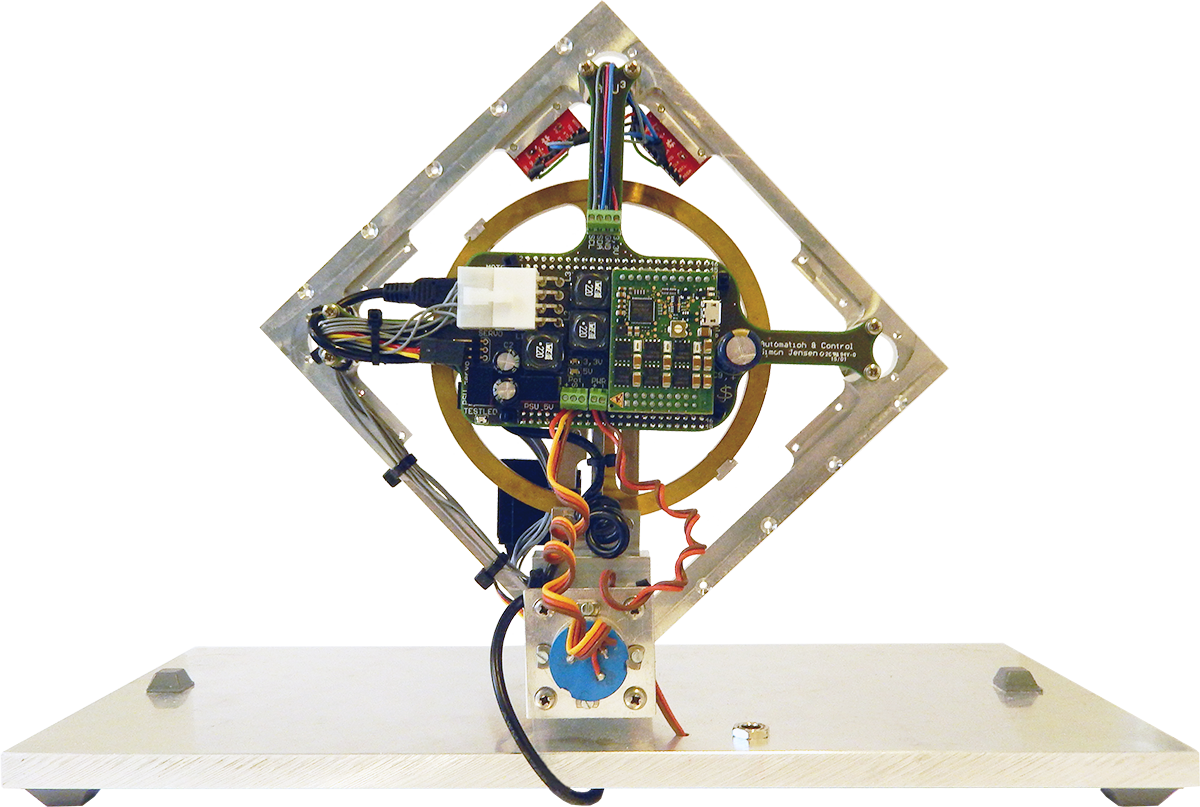
\includegraphics[width=0.95\textwidth]{figures/Cubli-1}
\label{fig:forside}
\end{figure}
  \vspace{0.6 cm}
  \begin{center}
    {\large
      6. Semester Project Report %Insert document type (e.g., Project Report)
    }\\
    \vspace{0.2cm}
    {\Large
      Group 16gr630%Insert your group name or real names here
    }
  \end{center}
  \begin{center}
  Aalborg University\\
  Electronic Engineering \& IT\\
  Fredrik Bajers Vej 7\\
  DK-9220 Aalborg
  \end{center}
\end{titlepage}

\clearpage
	\pagestyle{fancy}
	%\small
%\begin{figure}[H] 
%	\centering
%	\includegraphics[scale=0.38]{figures/Cubli-7}
%\end{figure}\vspace{-18pt}\begin{figure}[H] 
%	\centering
%	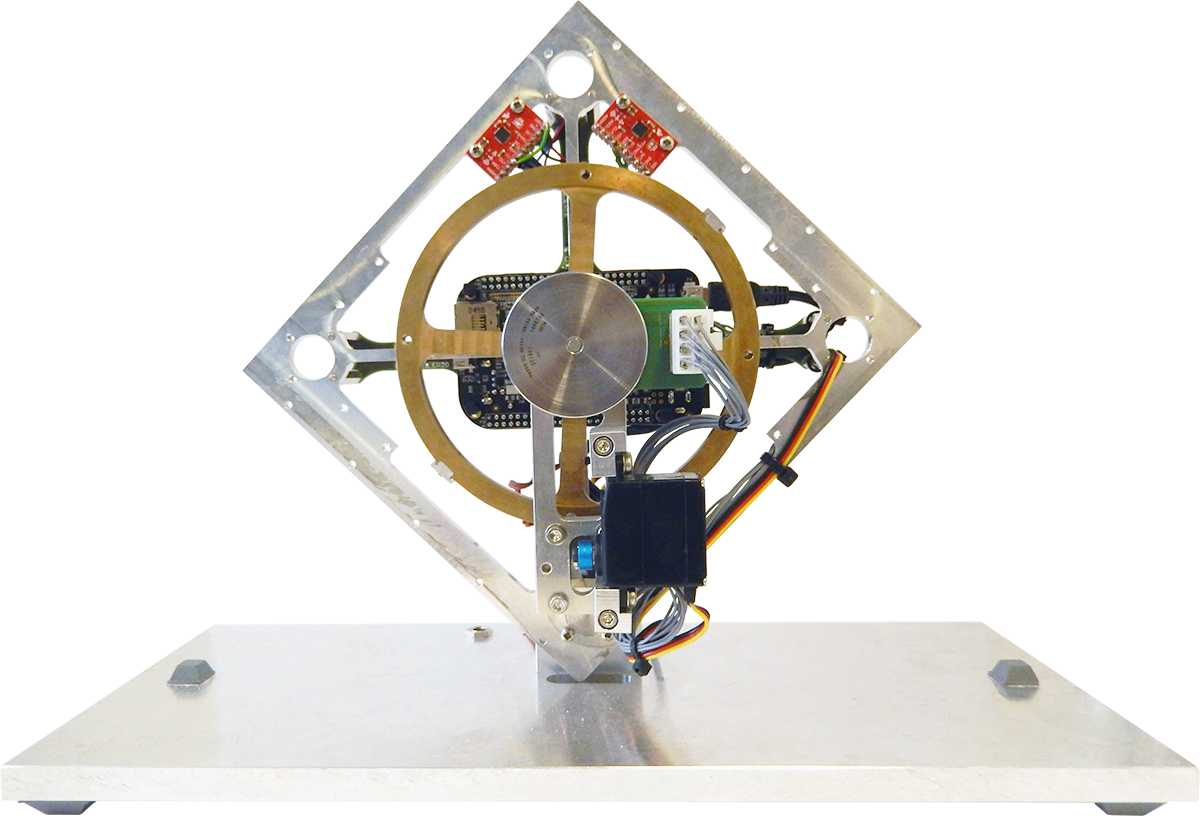
\includegraphics[scale=0.4]{figures/Cubli-2}
%\end{figure}\vspace{-18pt}\begin{figure}[H] 
%	\centering
%	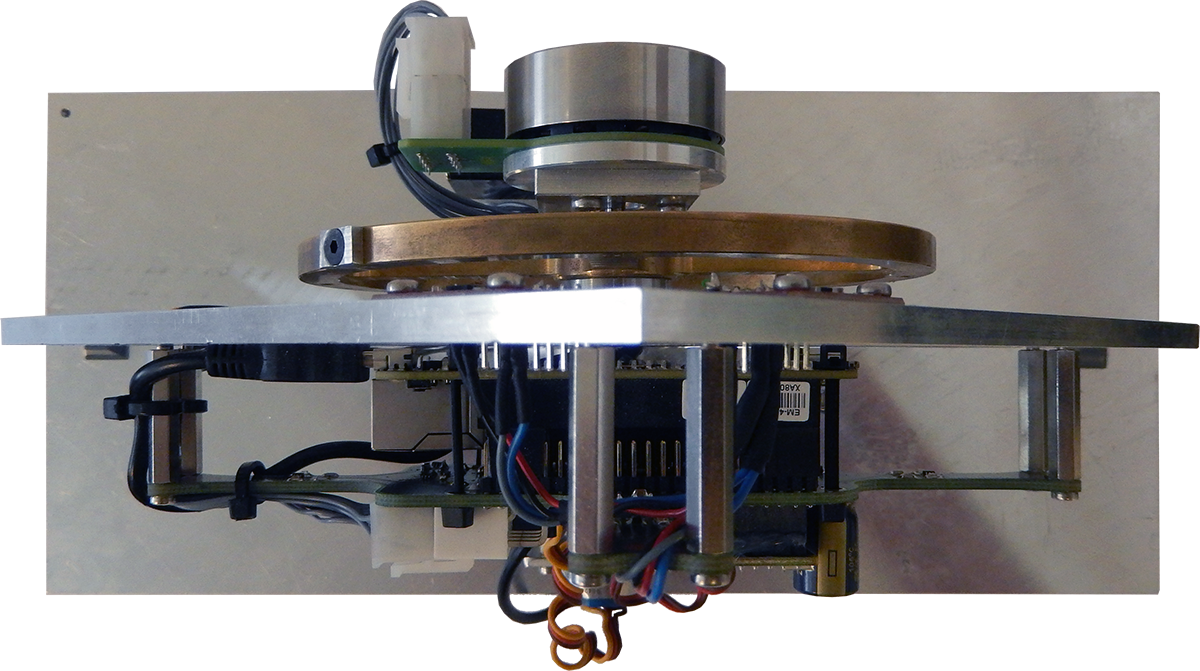
\includegraphics[scale=0.3, angle=180]{figures/Cubli-3}
%\end{figure}\vspace{-18pt}\begin{figure}[H] 
%	\centering
%	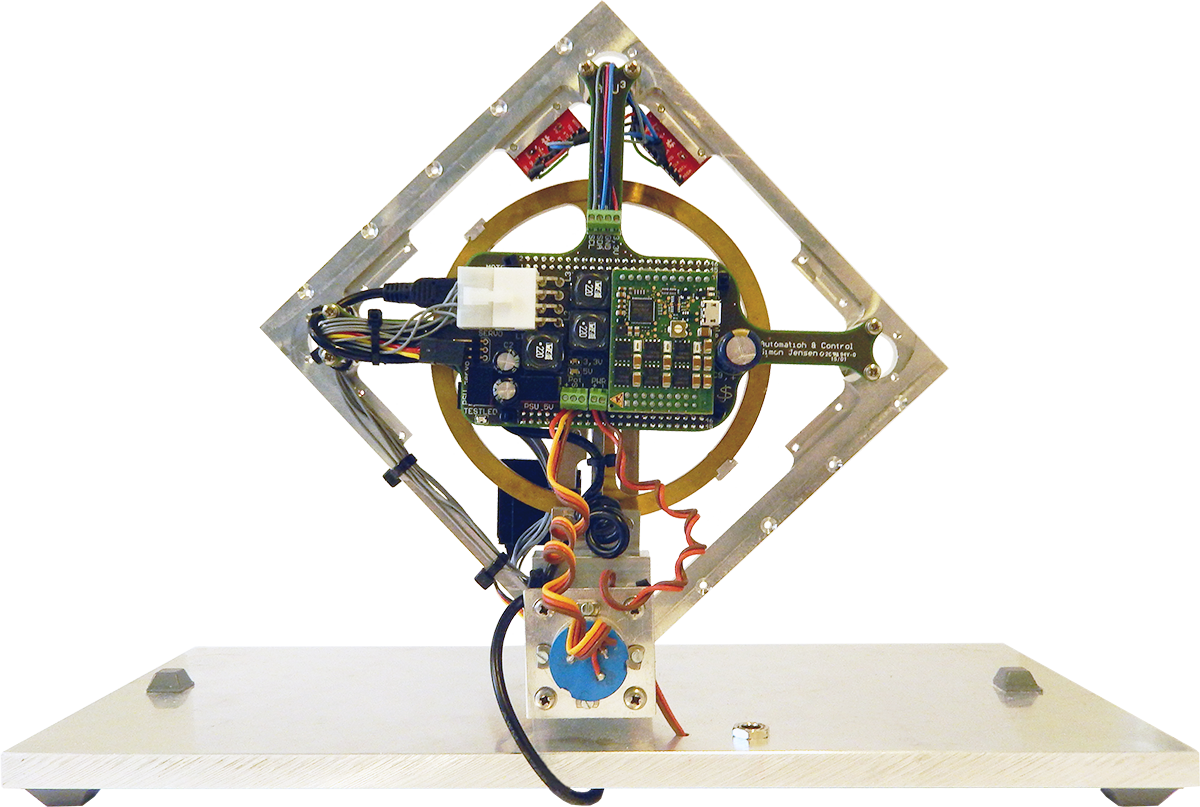
\includegraphics[scale=0.4, angle=180]{figures/Cubli-1}
%\end{figure}
\strut\vfill % push the content to the bottom of the page
\noindent Copyright \copyright{} Aalborg University 2016\par
\vspace{0.2cm}

\noindent This report is compiled in \LaTeX, originally developed by Leslie Lamport, based on Donald Knuth's \TeX. The main text is written in \emph{Latin Modern} pt 12, designed by Bogusław Jackowski and Janusz M. Nowacki. 
%The document is compiled via the website \url{www.overleaf.com}, an online collaborative based \LaTeX-editor with instant preview, which enables multiple persons to edit the document simultaneously.
Diagrams are made using Inkscape and Tikz.% Microsoft Visio. 
\clearpage
	%\begin{document} 
\thispagestyle{empty}
\begin{titlepage}
\begin{nopagebreak}
{\samepage 

\begin{tabular}{r}
\parbox{\textwidth}{  \raisebox{-15mm}{
\includegraphics[height=3cm]{figures/aaulogo-en.png}}
\hfill \hspace{2cm} \parbox{8cm}{\begin{tabular}{l} %4.90
{\small \textbf{\textcolor{aaublue}{\colorbox{white}{6\textsuperscript{th} Semester, Bachelor Project}}}}\\
{\small \textbf{\textcolor{aaublue}{School of Information and}}}\\
{\small \textbf{\textcolor{aaublue}{Communication Technologies}}}\\ 
{\small \textbf{\textcolor{aaublue}{Electronics and IT}}}\\
{\small \textcolor{aaublue}{Fredrik Bajers Vej 7C}} \\
{\small \textcolor{aaublue}{9220 Aalborg}} \\
{\small \textcolor{aaublue}{\emph{http://www.sict.aau.dk/electronics-and-it}}}
\end{tabular}}}
\end{tabular}

\begin{tabular}{cc}
\parbox{7cm}{

\textbf{Title:}

Cubli:\\
Dynamic Control of a Reaction Wheel Inverted Pendulum\\ %\fxnote{Input project title}\\

\textbf{Theme:}

\small{
BSc Project (Control Engineering)\\
}


\parbox{8cm}{


\textbf{Project Period:}\\
P6, Spring 2016\\
01/02/2016 - 25/05/2016\\
   
\textbf{Project Group:}\\
630\\ %\fxnote{Input group number}
  
\textbf{Participants:}\\
Bjørn Kitz\\
Julien Br\'ehin\\
Mikael Sander\\
Niels Skov Vestergaard\\
Noelia Villarmarzo Arruñada\\

\textbf{Supervisor:}\\
John-Josef Leth\\ %\fxnote{Input supervisor}
Palle Andersen
}\\

\textbf{Prints:} 8\\
\textbf{Pages:}\\
\textbf{Appendices:}\\
\textbf{Attached:} 1 CD\\
\textbf{Concluded:} 25/05/2016\\

\vfill } &
\parbox{7cm}{
  \vspace{.15cm}
  \hfill
  \begin{tabular}{l}
  {\textbf{Synopsis}}\bigskip \\
  \fbox{
    \parbox{6.5cm}{\bigskip
     {\vfill{\small Nowadays, the inverted pendulum is used in many applications and it is a classic research area in control theory which is still active.

The aim of this project is to model and analyze the behavior of a reaction wheel inverted pendulum, in the form of a one-frame Cubli, and to design a controller capable of balance it in equilibrium position. 

Moreover, a solution for measuring its angular position using only internally mounted sensors is to be designed to be able to use it in a full Cubli. 

Finally, the performance of all the designs are tested in simulation and in the real prototype to ensure that they fulfill the needed requirements.
     \bigskip}}
     }}
   \end{tabular}}
\end{tabular}} %\vspace{1cm}

\textit{\phantom{A}Publication of this report's contents (including citation) without permission\\ \phantom{A}from the authors is prohibited}\\

\end{nopagebreak}
\end{titlepage}
%\end{document}
	%%% Preface %%%
	%\cleardoublepage
	\textbf{\huge{Preface}}
\\
\\

\vspace{-12 pt}
\lipsum[3]\fxnote{Write prephase}

\textbf{Reading Instructions}
\vspace{-10 pt}
\begin{itemize}
\item[-] \lipsum[6]\fxnote{Write reading instructions}
\end{itemize}

%
\textbf{Text by:}\\
\vspace{-12 pt}
\begin{table}[H]
	\centering
		\begin{tabular}{c c c}
			\underline{\phantom{JAERJAERJAERJAERGO}} & \phantom{cookies} & \underline{\phantom{JAERJAERJAERJAERGO}} \\
			Bjørn Kitz			& \phantom{cookies} & Julien Br\'ehin		\\
			&&\\
			\underline{\phantom{JAERJAERJAERJAERGO}} & \phantom{cookies} & \underline{\phantom{JAERJAERJAERJAERGO}} \\
			Mikael Sander			& \phantom{cookies} & Niels Skov Vestergaard		\\
			&&\\
	    \multicolumn{3}{c}{\underline{\phantom{JAERJAERJAERJAERGO}}}\\
	    \multicolumn{3}{c}{Noelia Villarmarzo Arruñada}\\				
		\end{tabular}
\end{table}
\pagebreak
	
	\pdfbookmark[0]{Table of Contents}{label: tableOfContents}
	\tableofcontents
	\cleardoublepage
	
	
	%%% Mainmatter Settings %%%
	\pagenumbering{arabic} %use arabic page numbering in the mainmatter
	\fancyfoot[RO,LE]{\thepage \text{ of} \pageref{LastPage}}
	\fancyfoot[RE,LO]{16gr630}
	\fancyhead[RE,LO]{}
	\fancyhead[RE,LO]{\color{aaublue}\small\nouppercase\leftmark} %even page - chapter title
	\pagestyle{fancy}
	
	%%% Part 1 %%%
	\part{Preanalysis}
	
	%---------- Chapter 1 ---------------------------------------- Introduction
	\chapter{Chapter 1}
We, as a group, wanted to work with an unlinear system for our bachelor project in control engineering. The choice fell on a form of inverted pendulum. It is a setup called Cubli.\fxnote{add picture of 3d cubli}
The Cubli is a cube that can jump up and balance on one of its sides or one of its corners.\cite{MGajamohan}
In this case the inverted pendulum setup is not controlled by a motor that moves the pendulum, but by a flywheel attached to the square frame. There is one for each of the three axis of motion. 
At AAU we have a one-dimensional setup, based on the Cubli idea. It consists of a metalframe with one flywheel. The idea is to balance the frame on one corner with the help of the flywheel by accelerating the wheel up and down.

	%\section{AAU Cubli}

	%\section{Section 2}
\subsection{Subsection 1.2.1}
\subsection{Subsection 1.2.2} %-------- For Overview, sometimes short headlines here works well
	
	%---------- Chapter 2 ---------------------------------------- Design Considerations
	\chapter{Design Considerations}\label{chap:designConsiderations}
% - Mechanical description of 3 dimensional cubli (focus: control)
%     - jump up on side
%     - jump up on corner 
%     - balancing on side
%     - balancing on corner
% - What have other cubli-makers achieved
%     - balance deviation (if moved x degrees away from equilibrium
%                          point - for how big x can it still find
%                          its equilibrium again)
%     - corner balance (duration?)
%     - general on stability
%         - Different slopes
%     - moving (rolling)
%     - spin

From the introduced applications both in modular robot design as well as planetary or asteroid exploration, a high controllability Cubli design is desired.
In a realization of a full functioning Cubli, different considerations regarding design and overall functionalities must be taken into account. Later in this chapter restrictions are considered regarding the features to implement in this project.

% The setup for this project is given by the university, which means that some considerations must be taken into account when modelling the system and designing a controller to balance it.

% The full Cubli setup is a 3 dimensional cube, whose structure is a metallic frame. Inside the frame, three reaction wheels are mounted and driven by DC motors and a brake system and additionally there are different kind of sensors inside the frame, that are used to determine the position of the Cubli.
% %\fxnote{Look in source material what kind of sensors the cubli is using}

% The system is controlled by the use of reaction wheels, which make it able to balance on a side or a corner and to jump up from rest position when braking the wheels. It is also possible to make it move in one direction, if the control of the wheels is combined.% At this point, the Cubli can be considered a cube robot.\\

% On the other hand, the working setup that exists at Aalborg University (AAU) is composed by one of the sides of the 3D cube. One of the most important characteristics is that one of its corners is attached to a base plate. This feature limits the number of movements the Cubli can do, as it can only be balanced in one direction along a vertical plane.

% Since all the hardware is already built, the goal of the project is focused on deriving the model of the system, simulating it to compare it with the real Cubli and, moreover, on designing a controller which is able to balance it in the equilibrium position.

%At Aalborg University (AAU), there exists a working setup of a one-dimensional Cubli. The overall goals of this semester are to make a model of a system, to simulate this model and then to design and implement a controller for that system. Students on this semester are encouraged to work with pre-made setups, since the focus is rather on the control engineering than the hardware solution.\fxnote{moved the section directly from introduction. Will need a top to catch the previous chapter}

  \section{Desired Functionalities}\label{sec:mainFunctionalities}
In this section, a non exhaustive list of capabilities a Cubli prototype should have, is put forth.

A simple design method, for the Cubli to stand on one of its corners, is to make it jump to this position in two steps. First, it should be made to stand on one of its edges before going to a balancing position on a corner\fxnote{Add ref}.

Therefore, as a basic ability, the prototype should be able to jump onto any one of its edges.
By rotating one of its reaction wheels to a determined and controlled velocity and braking it suddenly, it should be able to raise the cube to an unstable position on an edge, enough so that another controller can catch it around equilibrium position.\\
This second controller is essential to allow the prototype to keep balancing. It should react fast enough when put into action so that the Cubli does not fall again. With some more considerations regarding this controller's robustness, it should be possible to change the inclination of the surface under it to a certain extent.\\
In a similar fashion, the second step of the process consists of speeding up wheels and braking them one more time to raise the Cubli to one of its corners. The latter should finally be caught by a controller able to maintain it in this unstable equilibrium.

Once standing on a corner, a spinning functionality should allow the prototype to turn around itself.\\
This change in orientation also permits the Cubli to move in its environment by falling and raising repeatedly towards the desired direction.

With a cube, wires are not practical if the prototype has to move around. To ensure a complete autonomy, the prototype should be remotely controllable, i.e. it should be possible to ask it to run pre-defined routines (stand on an edge or a corner, spin, make a full turn, etc.) from a distant computer.\\
Moreover, it should be self-sustained by an internal battery able to run the main computer, the actuators and the sensors for a reasonable amount of time.

All these functionalities are potential features to implement. The next section sets some limits as to what is actually achieved for this project.    %-------- Main Functionalities
  \section{Prototype Restrictions}\label{sec:protoRestrictions}
After some potential functionalities have been described, it is necessary to put some restrictions to the scope of this project.

To achieve a full Cubli design, an intermediary step with a one-side prototype is chosen as the focus for this project. This is to simplify the design process of the model and the controller before scaling it to a full cube.\\
This simplified prototype consists of a single square face of a cube, later on called frame. It should have one reaction wheel to raise it and a baseplate to which the frame is fixed so it only has one degree of freedom.

With only one frame, the prototype cannot spin around itself nor move as described in \secref{sec:mainFunctionalities}. Instead of balancing up in two steps, the frame can only balance on its corner which is comparable to getting the cube to balance on its edge.\\
The jump-up of the cube is also set aside, since it is considered out of scope for this Bachelor project.

Concerning the wireless capabilities of the prototype, since it is only going to be built as a single frame in this project, the need for power autonomy and remote communication is not critical for it to work properly. Moreover, wireless communication and hardware design are also out of scope for this Control Engineering project. This means the system will be powered by an external power supply and communication will be done by physically connecting to the prototype.

Noncritical functionalities are now set aside. The remaining focus is put on the control of a balancing single frame that is scalable to a cubic model.

At Aalborg University (AAU), there exists a working setup of a one-side Cubli. The overall goals of this semester are to make a model of this system, to simulate the model and then to design and implement a controller for it to balance around its equilibrium point. Furthermore, the prototype should be able to balance even when its baseplate is inclined.
In the next chapter, the available Cubli setup is described in more detail.

% With only two dimensions

% first step: 2D
% spin and move -> not yet in 3D
% jump up and balance on corner -> not yet in 3D but similar principle as raising it on its edge
% jump up on edge -> out of scope for this semester
% wireless: wifi communication is not crucial for it to work and outside of semester scope
%         + power autonomy is out of scope for the semester, not crucial and demands a very powerful battery

% => Use the university 2D prototype with hardware and base software available
% => Make a model of it, simulate it, control it, measure it and improve it  %-------- Main Functionalities

	%---------- Chapter 3 ---------------------------------------- System Description
	\chapter{System Description}
One-frame Cubli is a non-linear unstable system which is capable of laying on one of its corners as long as it is properly controlled, using the inertia created in the reaction wheel present in the setup.

This system is composed by several hardware parts, listed in the following table. \fxnote{insert correct part names} \fxnote{Include picture of the real model, mark all the parts in the picture}

\begin{table}[H]
	\begin{tabular}{|l|p{4.5cm}|}
		\hline %-----------------------------------------------------------------------------------
		\textbf{No.} &\textbf{Part} 			\\
		\hline %-----------------------------------------------------------------------------------
		1            & Frame           			\\
		\hline %-----------------------------------------------------------------------------------
		2            & Reaction wheel      		\\
		\hline %-----------------------------------------------------------------------------------
		3            & Controller (BeagleBone)  \\
		\hline %-----------------------------------------------------------------------------------
		4            & Potentiometer			\\
		\hline %-----------------------------------------------------------------------------------
		5            & IMU          			\\
		\hline %-----------------------------------------------------------------------------------
		6            & Brushless DC-motor   	\\
		\hline %-----------------------------------------------------------------------------------
		7            & Motor control board     	\\
		\hline %-----------------------------------------------------------------------------------
		8            & Jump brake		    	\\
		\hline %-----------------------------------------------------------------------------------
	\end{tabular}
	\caption{Main parts of the Cubli setup}
\label{TableAAUCubliComponent}
\end{table}

	\section{Mechanical Components}
The frame and the reaction wheel constitute the mechanical parts of the system.
\subsection{Frame}
The frame is made of aluminum with dimensions 17x16x0,5 \si{cm}  with two cross connections between opposing corners. To keep the weight down on the frame, a large area of the frame is milled out. That composes the body of the Cubli.\\
As it can only be balanced in one direction, it is attached to the base on one of its vertices to avoid it from falling in any of the other directions.
%It plays an important role since it acts like the inverted pendulum of the system and, moreover, all the electronics and the motor needed are attached to it.\fxnote{Isn't the motor rather attached to the wheel (both in reality and in the model) ? J.}
%This last aspect has to be taken into account when finding the model, as its moment of inertia, center of gravity and mass change.
\subsection{Reaction Wheel}
%A reaction wheel is a device used in many applications, such as attitude control in spacecrafts, when a change in rotation or keeping a certain attitude is needed.\fxnote{source?}
%The use of this kind of wheels allows these small variations in the rocket orientation, and thus reducing fuel needed to do this task.\fxnote{Do we really want a comparison with rockets or satellites?}
In the case of the Cubli, the reaction wheel is made of brass with most of the mass in a ring at its outer edge and two cross connections through its center.
The reaction wheel is coupled to the axis of a motor, through its center of rotation. When the wheel turns, its change of velocity creates a torque on the system that is transmitted with opposite direction to the body due to the conservation of angular momentum.		%-------- Mechanical Components
	\section{Main Boards}
On the prototype a microcontroller provides the main computing power and controls the system through the connecting and breakout board directly attached to the frame.

\subsection{Microcontroller}
The microcontroller used on this system is a BeagleBone Black, which is in charge of managing the data from the motor and the sensors and of calculating the required control action.\\
It uses an ARM processor at a clock frequency of \SI{1}{GHz} and has a large amount of general purpose inputs and outputs, of which some of them support the \si{I^2C} protocol or include an Analogue to Digital Converter (ADC).\\
%In order to use the data from the sensors it has to be sampled by the ADC in  the BeagleBone. 
The ADCs of the BeagleBone have a 12-bit resolution that is limited to a range of \si{0 - 1,8\ V}. The fastest sampling time it can provide is \si{125} \si{ns}\cite{Cameon}.

\subsection{Connecting and Breakout Board}
This board is used for power distribution with different voltages sent to each unit. There is also a built-in gain for the potentiometer, configured for the range of the BeagleBone Black ADC's and the possible positions that the frame can have. The schematics can be found in \appref{app:ConnectingBreakoutBoard}.

%From the schematic of the connecting and breakout board the gain has been built to have a gain of 3.\fxnote{It would be nice if the mention of the gain value were put with the initial statement that there is one instead of having a `cutting' paragraph in between. J.}				      %-------- Controller
	\section{Actuators}\label{sec:Motor}
There are two actuators in the system, a brushless DC-motor as the main actuator which is used to apply the required control action and aservo motor, which can be used to brake the wheel in order to raise the frame.

\subsection{Brushless DC-Motor}
The brushless DC-motor is attached to the wheel and it is in charge of providing the required torque to the system.
It is an EC 45 flat 50 Watt (part no. 251601), which has additional features such three Hall effect sensors for angular velocity measurements.
%can take a nominal current of 2.33 A, and 23 A at very short peaks.It has a mechanical time constant of 12,4 ms \cite{MaxonMotors}. The nominal current puts a limit on the control signal that can be sent to the motor control board.\fxnote{Should this control signal be mentioned here?}.
%\fxnote{Should there be made a table listing the motors data instead of writing a paraghap with the info?}
Table~\ref{BrushlessDCMotorTable} contains some of the characteristics for this motor.

\begin{table}[H]
	\centering
	\begin{tabular}{|p{4.8cm}|p{3.3cm}|}
		\hline%------------------------------------------------------------------------------------
		\textbf{Motor Data}                        &  \textbf{Value} \unitWh{Unit}  \\
		\hline%------------------------------------------------------------------------------------
%		Max voltage                               &  24 \unitWh{V}  	\\
%		\hline%------------------------------------------------------------------------------------
		Nominal current                   		  &  2,33 \unitWh{A}	\\
		\hline%------------------------------------------------------------------------------------
		Motor constant (\si{K_t})				 &  33,5 \unitWh{N\cdot m \cdot A^{-1}}  \\
		\hline%------------------------------------------------------------------------------------
		Mechanical time constant                 &  12,4 \unitWh{ms}  \\
		\hline%------------------------------------------------------------------------------------
	\end{tabular}
	\caption{Important parameters of the brushless DC-motor}
	\label{BrushlessDCMotorTable}
\end{table}


\subsection{Motor Control Board}
There is a motor control board, Maxon ESCON Module 50/5, connected between the BeagleBone and the brushless DC-motor, and it is specifically made to work with ESCON motors.

The following table shows some of the main characteristics of the board.

\begin{table}[H]
	\centering
	\begin{tabular}{|p{7cm}|p{2.3cm}|}
		\hline%------------------------------------------------------------------------------------
		\textbf{Characteristics}                 &  \textbf{Value} \unitWh{Unit}  \\
		\hline%------------------------------------------------------------------------------------
		Nominal output current                   &  5 \unitWh{A}  	\\
		\hline%------------------------------------------------------------------------------------
		Peak current (<20 s)                     &  15 \unitWh{A}	\\
		\hline%------------------------------------------------------------------------------------
		Current control PWM frequency 				   &  53,6 \unitWh{kHz}  \\
		\hline%------------------------------------------------------------------------------------
		Sample Rate of PI current controller     &  53,6 \unitWh{kHz}  \\
		\hline%------------------------------------------------------------------------------------
	\end{tabular}
	\caption{Important parameters of the motor control board}
	\label{MotorControlBoardTable}
\end{table}
%The PWM signal has a range of 10 \% to 90 \%. 
%Inside the board is a 4-quadrant configuration.\\
The motor control board can be configured with a program provided by Maxon called ESCON studio.\cite{ESCONStudio}\\ 
The board is set to run with a closed loop control for the current. It is assumed that the reference current is the one given to the motor so the loop can be seen just as a unit gain. This assumption is validated through a test described in \appref{app:motorCurrentTest}, where it can be seen that both currents can be assumed to be equal.

\begin{figure}[H]
	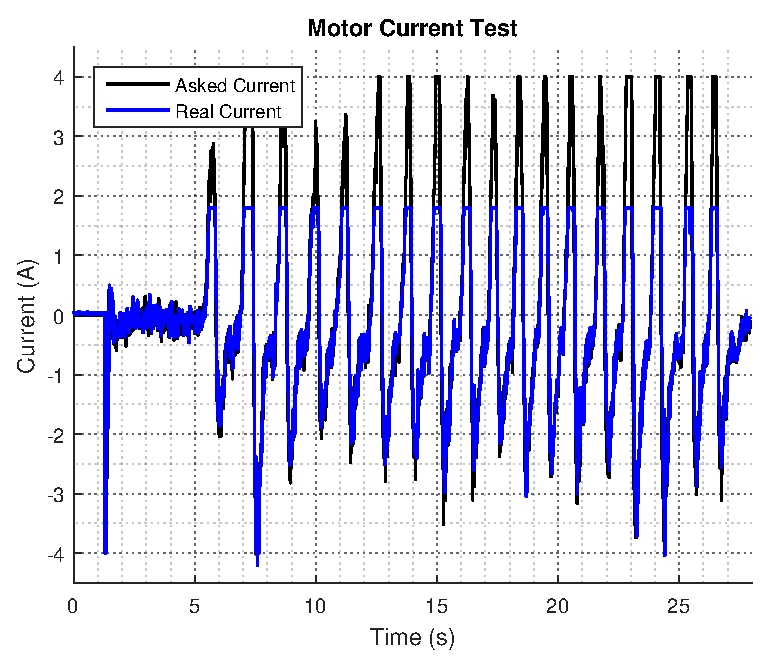
\includegraphics[scale=.65]{figures/motorCurrentTest}
	\centering
	\caption{Result of the test done to the motor to check that the reference current }
\end{figure} \label{motorCurrentTest2}

The reference current is sent to the control board as a PWM signal, whose duty cycle is configured within the range of 10 \% to 90 \% corresponding to \SI{4}{A} at 90 \% and \SI{-4}{A} at 10 \%. All the configurations can be seen \appref{MaxonControlESCON}.


\subsection{Braking System}
There is a braking mechanism included in the system, which can be used to make the frame go from resting position to vertical position.

To perform this task the brushless DC-motor spins up the reaction wheel and when it has enough kinetic energy the braking mechanism suddenly brake it, using for this task a Hitec HS225 Mighty Mini Servomotor. The inertia of the wheel is thus transfered to the frame, in order to raise it to standing position.

%The brake system is however not used in this project, since the jump up procedure is out of its scope.

%\fxnote{For gods sake fix this table!..:p}
%\begin{table}[H]
%	\centering
%	\begin{tabular}{|l|llll|}
%		\hline%------------------------------------------------------------------------------------
%		\textbf{Characteristics}           & \textbf{Values} &                      &  &\\
%		\hline%------------------------------------------------------------------------------------
%		Reaction time                      & @\SI{4,8}{V}    &\si{0,14/60} \si{s\cdot deg^{-1}} &and @\SI{6,0}{V} \si{0,11/60} &\si{s\cdot deg^{-1}} \\
%		\hline%------------------------------------------------------------------------------------
%		Speed                              & @\SI{4,8}{V}    &\SI{7,48}{rad\cdot s^{-1}} &and @\SI{6,0}{V} \si{9,52} &\si{rad\cdot s^{-1}}             \\
%		\hline%------------------------------------------------------------------------------------
%		Torque                             & @\SI{4,8}{V}    &\SI{3,9}{kgF\cdot cm} &and @\SI{6,0}{V} \si{4,8} &\si{kgF\cdot cm} \\
%		\hline%------------------------------------------------------------------------------------
%		Size                							 &  \multicolumn{4}{l|}{\si{32,26\ x\ 16,76\ x\ 31,00} \si{mm}}             \\
%		\hline%------------------------------------------------------------------------------------
%		Weight                             &  \SI{27,94}{g}  &                       &     &        \\
%		\hline%------------------------------------------------------------------------------------
%	\end{tabular}
%	\caption{Hitec HS225 Mighty Mini Servomotor Specifications}
%	\label{HitecHS225Servomotor}
%\end{table}					        %-------- Motor and Control Board
	\section{Sensors}
\label{sec:Sensors}

\subsection{Potentiometer}
The potentiometer is a precision potentiometer with a continuous turning and the text on it is: 65383-1-103 LIN \si{\pm1,0\%} RES 10K \si{\pm10\%} 9642EY. 

\subsection{IMU type MPU-6050}
  
The Motion Processing Unit (MPU) is a triple axis accelerometer with a gyro mounted on the breakout board from SparkFun. This is also called 6 Degrees of Freedom (6-DOF).

The MPU 6050 is a sensor based on Micro Electro Mechanical Systems (MEMS) technology. This chip uses Inter Integrated Circuit (I2C) protocol for communication, and is using I2C speed op to 400 kHz. 

The unit have a built in Digital-output temperature sensor for more precision measurement, embedded algorithms for run-time bias and compass calibration so no user calibration are required.
The unit collects gyroscope and accelerometer data while synchronizing data sampling at a user defined rate. 

For more precision measurement of the gyroscope and accelerometer, the unit can be programmed for the measurement of different intervals for the gyroscope from ±250 to ±2000 Degrees Per Second (DPS) and for a accelerometer range of ±2 g to ±16 g. 

The unit have built in 16-bit ADC converters for digitizing the gyroscope and accelerometer outputs and a digitally low-pass filter that can be programmed.

MPU-6050 have a buffer of 1024 Byte. The buffer is First In First Out (FIFO) type and is reducing timing requirements on the system processor.

The Digital Motion Processor (DMP) is capable of processing, so the Digital-output of the unit can be calculated as 6-Axis or 9-Axis MotionFusion on the unit. The output-data can come as rotation matrix, quaternion, Euler Angle, or raw data format. 

The MPU’s calculated output to the system processor can also include heating data from a digital 3-axis third party magnetometer.



\subsection{Planning of different test.}
The Cubli is analyzed so the parameters is confirmed and also to find the changes that have been made after the electronic board has been added to the frame during the last parameters measurement. For this reason, different tests will be made on the Cubli to find the different parameters and sensor inputs that will be used in making a model of the system.

The objective of this test is to find the linearity of the potentiometer and find the outer range of the frame rotation in degrees and potentiometer and BeagleBone Black A/D converter value, and the same for the balancing point, and at the same time get the new parameters of the frame like the weight and the placement of center of mass.


\subsection{Analyze the Potentiometer}
The potentiometer is placed at the corner of the frame which is fixed to an axis and it can be used to measure the actual position of the frame.\\
However its use is restricted to the one-dimensional Cubli, as it is attached and gives only an angle in relation to the base, which is not present in the 3D case.\\
In the project the potentiometer is used to test the dynamics of the Cubli and for feedback in the initial controller design.\\
Since the tests and feedback dependent on the reliability of the potentiometer, different tests are carried out on the potentiometer.
Test to find the voltage to angle conversion along with potential offset, see \appref{potentiometerRes}.

\begin{minipage}{\linewidth}
  	\begin{minipage}{0.45\linewidth}
  		\begin{figure}[H]
  			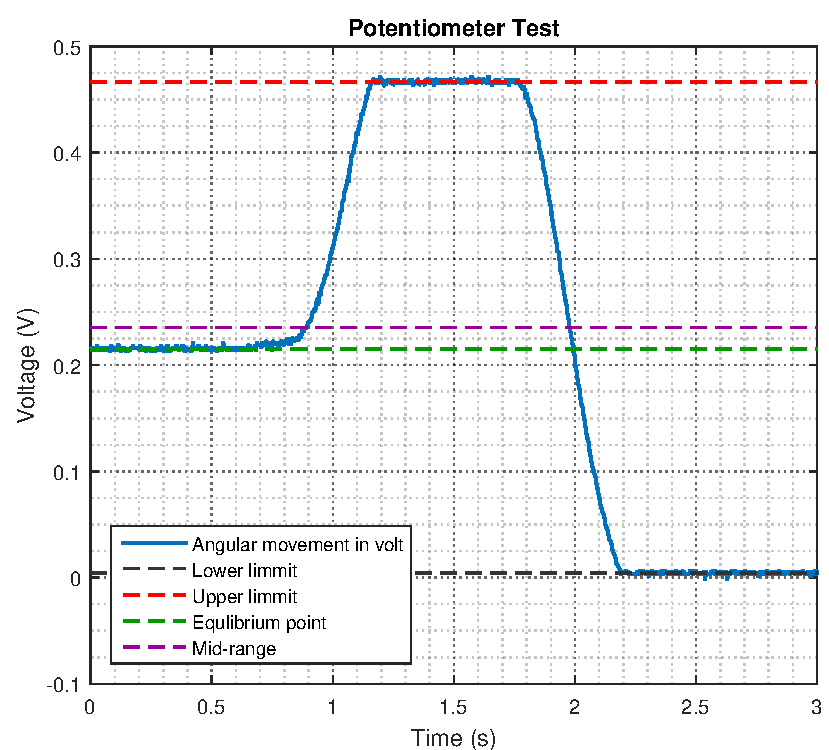
\includegraphics[scale=.5]{figures/PotentiometerResolution}
  			\centering
  			\captionsetup{justification=centering}
  			\captionof{figure}{\\Potentiometer measurements in volts}
  			\label{PotentiometerResolution}
  		\end{figure}\vspace{-5mm}
  	\end{minipage}
  	\hspace{0.03\linewidth}
  	\begin{minipage}{0.45\linewidth}
  		\begin{figure}[H]
  		%\vspace{.5cm}
  			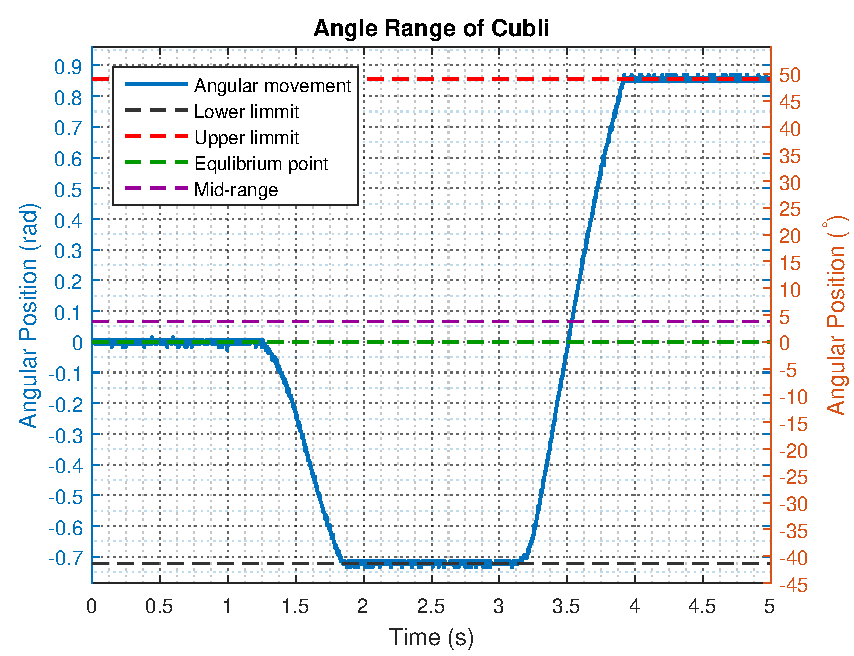
\includegraphics[scale=.5]{figures/PotentiometerResolutionDegRad}
  			\centering
  			\captionsetup{justification=centering}
  			\vspace{-.5cm}
  			\captionof{figure}{\\Potentiometer measurements converted to radians and degrees}
  			\label{PotentiometerResolutionRadDeg}
  		\end{figure}\vspace{-5mm}
  	\end{minipage}
\end{minipage}

The results of this test is shown above in \figref{PotentiometerResolution}, where the reference lines reveals an offset between the middle of the range and the equilibrium point of the Cubli frame.\\
This offset, also seen angle offset on \figref{PotentiometerResolutionRadDeg}, exists in the physical position of the frame. When the frame is standing in its equilibrium position it is displaced by approximately \si{3,9} degrees due to uneven distribution of mass around its center.\\
This results in a \si{48,9} degree range to one side of the optimal position and \si{41,1} degrees on the other\fxnote{STILL INVESTIGATING. IS NOT THAT UNEVEN AFTER ALL}.\\
To avoid complications it is chosen that the angle-offset must be accounted for such that the equilibrium position of the frame is at angle 0.

%Equilibrium point has been tested to have a range of 1 degree and the angle between the base and the frame is 42,5 degree. To avoid complications it is chosen that the angle-offset must be accounted for such that the equilibrium position of the frame is at 0 degree angle. This results in a 48,9 degree range to one side of the optimal position and 41,1 degree on the other.

The result gives an almost straight line well below of the 1 procent linearity of the potentiometer, but at a certain angle the potentiometer have an area where the measurement is deviating. The reason for this deviation is that it is a continuous rotating potentiometer and hit the point where it changes. A way to correct this problem is to turn the potentiometer a bit.\fxnote{Inset the to pictures} 

Testing the Linearity by measuring every 10 degree the value of the potential meter around Equilibrium point.

Equilibrium point have a range of 1 degree this is due to friction in the barreling.
\fxnote{make a table with important info}

\fxnote{the strange number from the code "16384" comes from datasheet, B}

                %-------- Sensors
	\section{Code Base}\label{sec:codeBase}
More than the physical setup, a certain amount of code allowing to run controllers on the present hardware is also available. \\
Written in C\texttt{++}, it comprises all the drivers necessary to interface the BeagleBone board with the motor and all the different sensors described above, in \secref{sec:Motor} and \secref{sec:Sensors}.

The actual controllers which make the Cubli stand up on its corner, are all composed of two or three files in a folder named \textit{controller/controller\_code/}. Each controller has to implement three functions, as shown in \autoref{lst:StandardControllerInterface}.
%
\lstset{language=C++, caption={Code snippet of the standard controller interface}, label=lst:StandardControllerInterface}
\begin{lstlisting}
  /**
   *  Runs the actual controller on the given feedback(s) and the pre-defined input(s).
   *  Takes the sampling time and a 3x1 vector x_hat containing the feedbacks 
   *  (processed data from the sensors):
   *              0: angular position of the frame
   *              1: angular velocity of the frame
   *              2: angular velocity of the wheel.
   *  Returns the output which should be applied to the actuator (current -> motor)
   */
  extern CONTROLLER_OUTPUT_struct_T AAU3_CUSTOM_CONTROLLER(real_T Ts, 
                                                   const real_T x_hat[3]);
  /**
   *  Initializes the controller parameters (gain, polynomials coefficients)
   *  Has to be called only once, before running the controller itself.
   */
  extern void AAU3_CUSTOM_CONTROLLER_initialize(void);
  /**
   *  Does whatever is needed (if needed) to stop the controller
   */
  extern void AAU3_CUSTOM_CONTROLLER_terminate(void);

\end{lstlisting}
This is a default model based on the way MATLAB auto-generates controller code into C\texttt{++} files. This model shall be used in this project as a general reference, to keep some common structure between the different controllers to be implemented. However, it is possible to adapt the arguments and the returned variables depending on the needs. Moreover, MATLAB auto-generation of code is not used in this project.

The file \textit{controller/controller\_test.cpp} contains the core part of the controllers operation. One of its functions, \lstinline{void ControllerTest::runController(ControllerArgs* args)}, is called at some regular pre-defined intervals which is the desired sampling time. This initializes the available controllers, retrieves and processes the data from the sensors, and finally uses the controller code to compute the output current to send to the motor. This updated output current is actually sent at the beginning of the next call.

It is important to note that the whole code is intended to run on the Beaglebone Black. Indeed, the latter uses an ARMv7 processor architecture, which requires the program to be compiled either directly on a computer with similar architecture which might be slow, or on another standard PC with a cross-compilation toolchain.
\\\\					      %-------- Code Base
	In this chapter, the Cubli setup has been described from the mechanical parts to the electronics components and to the software code base.
The next chapter presents a mathematical approach for the description of the system and its behavior.                   %-------- Chapter's tail
	
	%---------- Chapter 5 ---------------------------------------- System Modelling
	\chapter{System Modelling}
With the given setup being described, it is necessary to study its natural behavior in more details by deriving a model of this system. This chapter shows the process used to put up this model and an analysis of its pertinence. With this model, it shall be possible to determine realistic requirements for the controllers to implement in this project, see \chapref{chap:specifications}.

As a start to this modelling, a mechanical drawing of the Cubli showing angles and coordinate system conventions is seen in \figref{cubliMechanical}. A two-dimensional global coordinate system is chosen with its origin on the pivot point of the frame. Moreover, angles of the total body and the wheel count grow clockwise.

\begin{figure}[H]
 \centering
 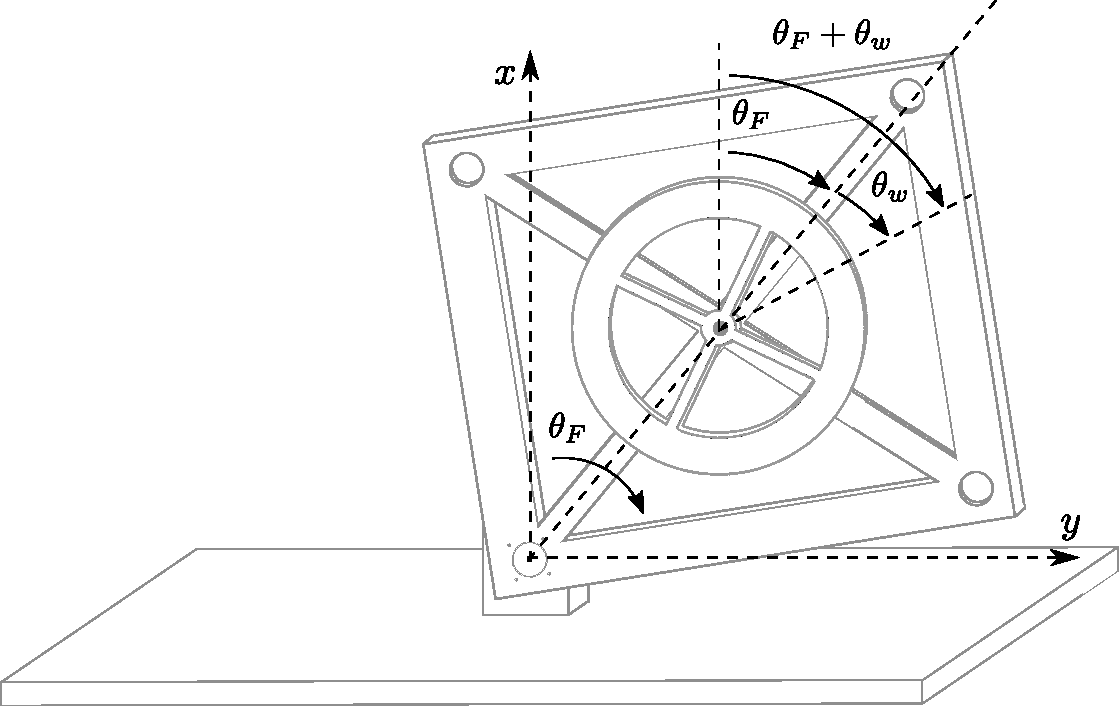
\includegraphics[scale=0.6]{figures/mechanicalSystem}
 \caption{Mechanical drawing of the Cubli, including angle coordinate system conventions}
 \label{cubliMechanical}
\end{figure}

%As shown in \figref{cubliMechanical}, 
In the next section, a complete model of the given setup is derived from Newton's Second Law of motion and rotation.
	\section{Derivation}
To derive the modelling equations for the Cubli system from Newton's Second Law, the former is split up into its two moving parts as seen in \figref{freeBodyFrame} and \figref{freeBodyWheel}.

  \begin{minipage}{\linewidth}
  	\begin{minipage}{0.45\linewidth}
  		\begin{figure}[H]
  			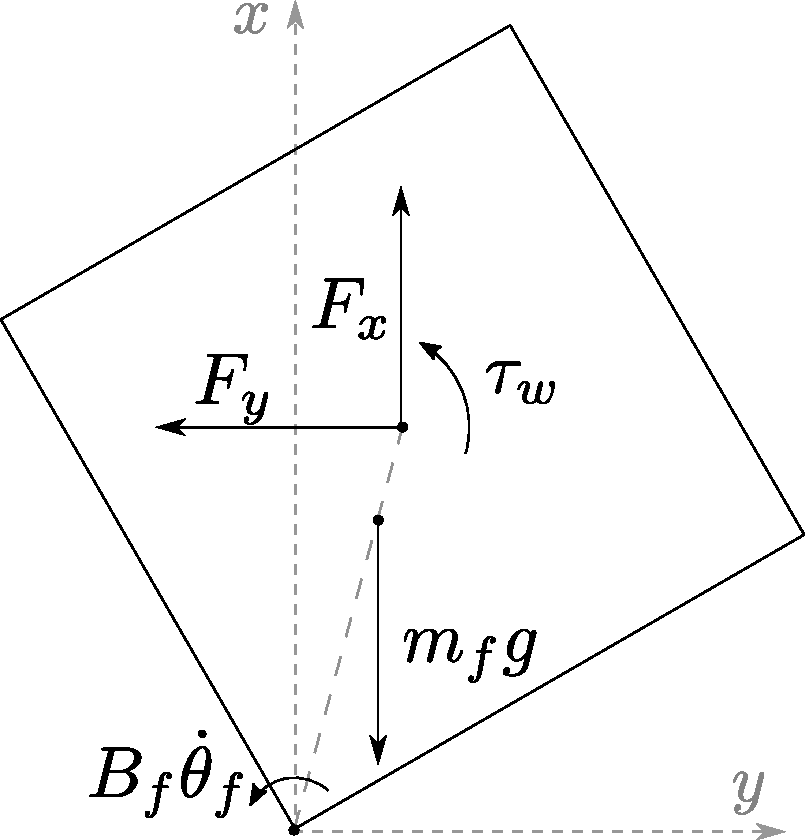
\includegraphics[scale=.5]{figures/freeBodyFrame}
  			\centering
  			\captionsetup{justification=centering}
  			\captionof{figure}{\\Free body diagram of the frame of the Cubli}
  			\label{freeBodyFrame}
  		\end{figure}\vspace{-5mm}
  	\end{minipage}
  	\hspace{0.03\linewidth}
  	\begin{minipage}{0.45\linewidth}
  		\begin{figure}[H]
  			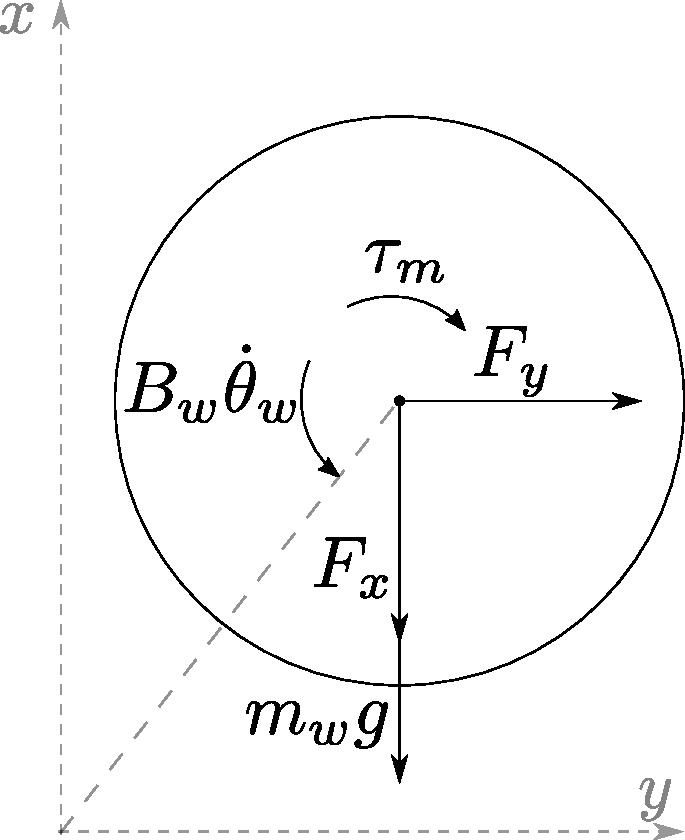
\includegraphics[scale=.53]{figures/freeBodyWheel}
  			\centering
  			\captionsetup{justification=centering}
  			\captionof{figure}{\\Free body diagram of the reaction wheel of the Cubli}
  			\label{freeBodyWheel}
  		\end{figure}\vspace{-5mm}
  	\end{minipage}
  \end{minipage}

The equation for the frame is deduced from the \figref{freeBodyFrame}.
\begin{flalign}
  \eq{J_F \vec{\ddot{\theta}_F}} { -B_F \vec{\dot{\theta}_F} + \vec{l_F} \times (m_F\cdot \vec{g}) + \vec{l_w} \times \vec{F} - \vec{\tau_m} + B_w \vec{\dot{\theta}_w}} \unit{N\cdot m}
\label{frameModelEq}
\end{flalign}
%
\hspace{6mm} Where:\\
\begin{tabular}{ p{1cm} l l l}
& \si{J_F} 					    	   & is the inertia of the frame                          &\unitWh{kg \cdot m^2} \\
& \si{\vec{\ddot{\theta}_F}} & is the angular acceleration of the frame             &\unitWh{rad \cdot s^{-2}} \\
& \si{B_F} 	                 & is the friction coefficient of the frame             &\unitWh{N \cdot m \cdot s \cdot rad^{-1}} \\
& \si{\vec{\dot{\theta}_F}}  & is the angular velocity of the frame                 &\unitWh{rad \cdot s^{-1}} \\
& \si{\vec{l_F}}             & is the length to center of mass of the frame         &\unitWh{m} \\
& \si{m_F}                   & is the mass of the frame                             &\unitWh{kg} \\
& \si{\vec{g}}							 & is the gravitational acceleration                    &\unitWh{m\cdot s^{-2}} \\
& \si{\vec{l_w}}             & is the length to center off mass of the wheel        &\unitWh{m} \\
& \si{\vec{F}}				  	   & is the force delivered to the frame from the wheel   &\unitWh{N} \\
& \si{\vec{\tau_m}} 	       & is the torque delivered by the motor        &\unitWh{N \cdot m} \\
& \si{B_w} 	                 & is the friction coefficient of the wheel             &\unitWh{N \cdot m \cdot s \cdot rad^{-1}} \\
& \si{\vec{\dot{\theta}_w}}  & is the angular velocity of the wheel with respect to the frame                 &\unitWh{rad \cdot s^{-1}} \\
\end{tabular}

The following equation is then derived from \figref{freeBodyWheel}:
\begin{flalign}
  \eq{ J_w (\ \vec{\ddot{\theta}_F} + \vec{\ddot{\theta}_w}\ ) } { \vec{\tau_m} - B_w \vec{\dot{\theta}_w }} \unit{N\cdot m }
\label{tauW}
\end{flalign}
\hspace{6mm} Where:\\
\begin{tabular}{ p{1cm} l l l}
& \si{J_w} 					    	   & is the inertia of the wheel                          &\unitWh{kg \cdot m^2} \\
& \si{\vec{\ddot{\theta}_w}} & is the angular acceleration of the wheel with respect to the frame             &\unitWh{rad \cdot s^{-2}} \\
\end{tabular}

In \eqref{frameModelEq} the term \si{\vec{l_w} \times \vec{F}} describes the torque delivered from the wheel to the frame, as it acts around the pivot corner of the frame. The vector \si{\vec{F}} is decomposed into to forces paralell to the axes, \si{F_x} and \si{F_y}, as seen on \figref{freeBodyFrame} and \figref{freeBodyWheel}. To be able to apply Newton's Second Law, expressions for both the x- and y-coordinate describing the position of the center of mass of the wheel are found.
%
\begin{flalign}
  \eq{x} { l_w \cdot cos( \theta_F ) } \unit{ m }\\
  \eq{y} { l_w \cdot sin( \theta_F ) } \unit{ m }
\label{xyCoordinate}
\end{flalign}
%
According to Newton's 2nd law of motion, \si{\sum F = m \cdot a}. Then to find \si{F_x} and \si{F_y}, the acceleration of the point at center of mass of the wheel must be known for both the x- and the y-direction. To achieve this the derivatives of the expressions for x and y in \eqref{xyCoordinate} are derived.
%
\begin{flalign}
  \eq{\dot{x}} { -l_w \cdot sin( \theta_F )\ \dot{\theta}_F } \unit{ m\cdot s^{-1} }\\
  \eq{\ddot{x}} { -l_w \cdot cos( \theta_F )\ {\dot{\theta}_F}^{\ \ 2} - l_w \cdot sin( \theta_F ) \ddot{\theta}_F } \unit{ m\cdot s^{-2} }
\label{xCoordinateDerivatives}
\end{flalign}
%
\begin{flalign}
  \eq{\dot{y}} { l_w \cdot cos( \theta_F )\ \dot{\theta}_F } \unit{ m\cdot s^{-1} }\\
  \eq{\ddot{y}} { -l_w \cdot sin( \theta_F )\ {\dot{\theta}_F}^{\ \ 2} + l_w \cdot cos( \theta_F )\ \ddot{\theta}_F } \unit{ m\cdot s^{-2} }
\label{yCoordinateDerivatives}
\end{flalign}
%
\Eqref{xCoordinateDerivatives} and \eqref{yCoordinateDerivatives} can now be used with Newton's 2nd law of motion, while also taking gravity into account in sum of forces, to derive \si{F_x} and \si{F_y}.
%
\begin{flalign}
  \eq{ -F_x -m_w \cdot g }{ m_w \cdot \ddot{x} } &\nonumber\\
  \eq{ F_x }{ - m_w \cdot \ddot{x} - m_w \cdot g} &\nonumber\\
  \eq{ F_x }{ m_w \cdot (\  l_w \cdot cos( \theta_F )\ {\dot{\theta}_F}^{\ \ 2} + l_w \cdot sin( \theta_F )\ \ddot{\theta}_F \ ) - m_w \cdot g} \unit{N}
\label{Fx}
\end{flalign}
%
\begin{flalign}
  \eq{ -F_y }{ m_w \cdot \ddot{y} } & \nonumber\\
  \eq{ F_y }{ -m_w \cdot (\ -l_w \cdot sin( \theta_F )\ {\dot{\theta}_F}^{\ \ 2} + l_w \cdot cos( \theta_F )\ \ddot{\theta}_F\ ) } & \nonumber\\
  \eq{ F_y }{ m_w \cdot (\ l_w \cdot sin( \theta_F )\ {\dot{\theta}_F}^{\ \ 2} - l_w \cdot cos( \theta_F )\ \ddot{\theta}_F\ ) } \unit{N}
\label{Fy}
\end{flalign}

The original objective was to evaluate the term \si{\vec{l_w} \times \vec{F}} in \eqref{frameModelEq}. Since the expressions for the two forces, \si{F_x} and \si{F_y}, that compose the vector \si{\vec{F}}, are found in \eqrefTwo{Fx}{Fy}, the vector product from \eqref{frameModelEq} is evaluated.

\begin{flalign}
  \si{\vec{l_w} \times \vec{F}} &=
    \begin{vmatrix}
      \ \si{\vec{\hat{i}}}                & \si{\vec{\hat{j}}}               & \si{\vec{\hat{k}}} \ \ \ \\ 
      \ \si{ l_w \cdot cos( \theta_F ) }  & \si{ l_w \cdot sin( \theta_F ) } & 0                  \ \ \ \\ 
      \ \si{ F_x }                        & \si{ F_y }                      & 0                  \ \ \  
    \end{vmatrix} \unit{N\cdot m}\\ \nonumber \\
  \si{ \vec{l_w} \times \vec{F} } &= 
    \begin{bmatrix}
      \ \si{ ( l_w \cdot sin( \theta_F) \cdot 0 - 0 \cdot F_y ) } \ \ \ \\
      \ \si{ ( l_w \cdot cos( \theta_F )\cdot 0 + 0 \cdot F_x  ) } \ \ \ \\
      \ \si{ ( l_w \cdot cos( \theta_F )\cdot F_y - l_w \cdot sin( \theta_F )\cdot F_x ) }
    \end{bmatrix} \unit{N\cdot m} \\ \nonumber\\
  \si{ \vec{l_w} \times \vec{F} } &= \si{ 0 \cdot \hat{i} + 0 \cdot \hat{j} + ( l_w \cdot cos( \theta_F )\cdot (m_w \cdot (\ l_w \cdot sin( \theta_F )\ {\dot{\theta}_F}^{\ \ 2} - l_w \cdot cos( \theta_F )\ \ddot{\theta}_F\ ))} \nonumber \\
  &\ \ \ \ \si{- l_w \cdot sin( \theta_F )\cdot (m_w \cdot (\  l_w \ cos( \theta_F )\ {\dot{\theta}_F}^{\ \ 2} + l_w \cdot sin( \theta_F )\ \ddot{\theta}_F \ )} \nonumber \\
  &\ \ \ \ \si{- m_w \cdot g) ) \cdot \hat{k}} \unit{N \cdot m}\\ \nonumber\\
  \eq{ \vec{l_w} \times \vec{F} }{ ({-l_w}^2 \cdot m_w \ddot{\theta}_F \ (cos^2(\theta_F) + sin^2(\theta_F)) + l_w\cdot sin(\theta_F)\ m_w \cdot g ) \cdot \hat{k}} \unit{N \cdot m}\\ \nonumber\\
  \eq{ \vec{l_w} \times \vec{F} }{ (-{l_w}^2 \cdot m_w \ddot{\theta}_F + l_w\ sin(\theta_F)\ m_w \cdot g ) \cdot \hat{k}} \unit{N \cdot m}
\label{vectorDecomposition3}
\end{flalign}

Since all torques only have a z-coordinate, \eqref{vectorDecomposition3} is inserted in \eqref{frameModelEq}, without vector-notation. Note that \si{\vec{l_F} \times (m_F\cdot \vec{g}) = (m_F \cdot l_F \cdot g \cdot sin(\theta_F)) \cdot \hat{k} }.
%
\begin{flalign}
	\si{J_F \cdot \ddot{\theta}_F} &= \si{- B_F \cdot \dot{\theta}_F + m_F \cdot l_F \cdot g \cdot sin(\theta_F)} \nonumber\\ 
	&\ \ \ \ \si{- m_w \cdot {l_w}^{2} \cdot \ddot{\theta}_F + m_w \cdot l_w  \cdot g \cdot sin(\theta_F) - \tau_m + B_w \cdot \dot{\theta}_w} \unit{N\cdot m}
\label{FrameEq2}
\end{flalign}
%
\begin{flalign}
	\eq{(J_F+m_w \cdot {l_w}^{2}) \cdot \ddot{\theta}_F} {- B_F \cdot \dot{\theta}_F + (m_F \cdot l_F + m_w \cdot l_w) \cdot g \cdot sin(\theta_F) - \tau_m + B_w \cdot \dot{\theta}_w} \unit{N\cdot m}
\label{FrameEq3}
\end{flalign}

Isolating \si{\ddot{\theta}_F} from \eqref{FrameEq3} gives the final expression for the rotational acceleration of the frame.
\begin{flalign}
	\eq{\ddot{\theta}_F} {\frac{- B_F \cdot \dot{\theta}_F + (m_F \cdot l_F + m_w \cdot l_w) \cdot g \cdot sin(\theta_F) - \tau_m + B_w \cdot \dot{\theta}_w}{J_F + m_w \cdot {l_w}^{2}}}  \unit{rad \cdot s^{-1}} 
\label{FrameEq4}
\end{flalign}

The equation above can be rearranged to clarify the effect that each variable exerts on the final acceleration of the frame.
\begin{flalign}
	\eqOne{\ddot{\theta}_F} {-\frac{B_F}{J_F + m_w \cdot l^2_w} \cdot \dot{\theta}_F + \frac{(m_F \cdot l_F + m_w \cdot l_w) \cdot g}{J_F + m_w \cdot l^2_w} \cdot sin(\theta_F)}
	\eqTwo{ - \frac{1}{J_F + m_w \cdot l^2_w} \cdot \tau_m + \frac{B_w}{J_F + m_w \cdot l^2_w} \cdot \dot{\theta}_w}   \unit{rad \cdot s^{-1}} 
\label{FrameEqFinal}
\end{flalign}

Once the acceleration of the frame is described by \eqref{FrameEqFinal} it is possible to derive an expression for the angular acceleration of the wheel with respect to its axis from \eqref{tauW}.
\begin{flalign}
	\eq{\ddot{\theta}_w} {\frac{\tau_m - B_w \cdot \dot{\theta}_w}{J_w} - \ddot{\theta}_F} \unit{rad \cdot s^{-1}} 
\label{WheelRotEq2}
\end{flalign}

Substituting \si{\ddot{\theta}_F} by the expression for the angular acceleration of the frame (\eqref{FrameEq4}) into \eqref{WheelRotEq2} gives the final description for \si{\ddot{\theta}_w}, as shown in \eqref{WheelRotEqFinal}.
\begin{flalign}
	\si{\ddot{\theta}_w} &= \si{\frac{\tau_m - B_w \cdot \dot{\theta}_w}{J_w}}\nonumber\\ 
	&\ \ \ \ \si{- \frac{(m_F \cdot l_F + m_w \cdot l_w) \cdot g \cdot sin(\theta_F) - \tau_m + B_w \cdot \dot{\theta}_w - B_F \cdot \dot{\theta}_F}{J_F+m_w \cdot {l_w}^{2}}} \unit{rad \cdot s^{-1}}
\label{WheelRotEq3}
\end{flalign}
%
\begin{flalign}
	\eqOne{\ddot{\theta}_w} {\frac{(J_w+J_F+{l_w}^{2} \cdot m_w) \cdot (\tau_m - B_w \cdot \dot{\theta}_w)}{J_w \cdot (J_F+m_w \cdot {l_w}^{2})}}
	\eqTwo{- \frac{(m_F \cdot l_F + m_w \cdot l_w) \cdot g \cdot sin(\theta_F) - B_F \cdot \dot{\theta}_F}{J_F+m_w \cdot {l_w}^{2}}} \unit{rad \cdot s^{-1}}
\label{WheelRotEq4}
\end{flalign}

\Eqref{WheelRotEq4} can be rearranged in the same way as \eqref{WheelRotFinal}.
\begin{flalign}
	\eqOne{\ddot{\theta}_w} {\frac{J_w+J_F+{l_w}^{2} \cdot m_w}{J_w \cdot (J_F+m_w \cdot {l_w}^{2})} \cdot \tau_m - \frac{(J_w+J_F+{l_w}^{2} \cdot m_w) \cdot B_w}{J_w \cdot (J_F+m_w \cdot l_w^{2})} \cdot \dot{\theta}_w }
	\eqTwo{- \frac{(m_F \cdot l_F + m_w \cdot l_w) \cdot g}{J_F+m_w \cdot {l_w}^{2}} \cdot sin(\theta_F) + \frac{B_F}{J_F+m_w \cdot {l_w}^{2}} \cdot \dot{\theta}_F} \unit{rad \cdot s^{-1}} 
\label{WheelRotFinal}
\end{flalign}

The final model of the system can be summarize with the following equations:

\footnotesize{\si{\ddot{\theta}_F = -\frac{B_F}{J_F + m_w \cdot {l_w}^2} \cdot \dot{\theta}_F + \frac{(m_F \cdot l_F + m_w \cdot l_w) \cdot g}{J_F + m_w \cdot {l_w}^2} \cdot sin(\theta_F) - \frac{1}{J_F + m_w \cdot {l_w}^2} \cdot \tau_m + \frac{B_w}{J_F + m_w \cdot {l_w}^2} \cdot \dot{\theta}_w} 	} \begin{flalign} \label{finalFrame} \end{flalign}
%
\footnotesize{\si{\ddot{\theta}_w = \frac{J_w+J_F+m_w \cdot {l_w}^{2}}{J_w \cdot (J_F+m_w \cdot {l_w}^{2})} \cdot \tau_m - \frac{(J_w+J_F+{l_w}^{2} \cdot m_w) \cdot B_w}{J_w \cdot (J_F+m_w \cdot  {l_w}^2)} \cdot \dot{\theta}_w - \frac{(m_F \cdot l_F + m_w \cdot l_w) \cdot g}{J_F+m_w \cdot {l_w}^{2}} \cdot sin(\theta_F) + \frac{B_F}{J_F+m_w \cdot {l_w}^{2}} \cdot \dot{\theta}_F}} \begin{flalign} \label{finalWheel} \end{flalign}
%
\fxnote{allign more beautifully}      %-------- Derivation
	\section{Linearization of the Model}
Now that a model of the Cubli frame is put forth in \eqref{FrameEqFinal} \fxnote{redo that reference, since we will be changing the equations in the previous subsection}, it is apparent that the system is nonlinear due to the term including \si{sin(\theta_F)}. In order to proceed with a simulation and controller design, it is convenient to first linearize the model. This is done by use of a Taylor series approximation.

Based on \eqref{FrameEq3} the system is described in an operating point, around which it varies with \si{\Delta \theta_F}.
%
\begin{flalign}
	\si{(J_F+m_w \cdot {l_w}^{2}) (\overline{\ddot{\theta}}_F + \Delta \ddot{\theta}_F )} &= \si{- B_F \cdot (\overline{\dot{\theta}}_F + \Delta \dot{\theta}_F) }   \nonumber\\
	&\ \ \ \ \si{+ (m_F \cdot l_F + m_w \cdot l_w) \cdot g \cdot sin(\overline{\theta}_F + \Delta \theta_F)} \nonumber\\
	&\ \ \ \ \si{- (\overline{\tau}_m + \Delta \tau_m) + B_w \cdot (\overline{\dot{\theta}}_w +\Delta \dot{\theta}_w)}  \unit{N \cdot m}\\
	\eq{(J_F+m_w \cdot {l_w}^{2}) (\overline{\ddot{\theta}}_F + \Delta \ddot{\theta}_F )}{ f( (\overline{\dot{\theta}}_F + \Delta \dot{\theta}_F), \ (\overline{\theta}_F + \Delta \theta_F), \ (\overline{\tau}_m + \Delta \tau_m),\  (\overline{\dot{\theta}}_w + \Delta \dot{\theta}_w) ) } \unit{N \cdot m}
\label{FrameEq4OperatingPoint}
\end{flalign}
%
%The operating point is chosen to be \si{\theta_F = 0}, which corresponds to the frame being in upright position, see \figref{cubliMechanical}.
The operating point is chosen as \si{\overline{\theta}_F} and \si{\overline{\theta}_w} and their derivatives being equal to 0. This corresponds to the frame being in the upright position, see \figref{cubliMechanical}. With the angels, velocities and accelerations being 0 the torque \si{\tau_m} is 0 as well.
Taking this into account and applying the Taylor series approximation yields the following.
%
\begin{flalign}
	\si{(J_F+m_w \cdot {l_w}^{2}) \Delta \ddot{\theta}_F } &= \cancelto{0}{\si{f( \dot{\theta}_F, \ \theta_F, \ \tau_m,\ \ddot{\theta}_w )}}   \nonumber\\
	&\ \ \ \ \si{+ \frac{\partial}{\partial \dot{\theta}_F} f\cdot \Delta \dot{\theta}_F + \frac{\partial}{\partial \theta_F} f\cdot \Delta \theta_F + \frac{\partial}{\partial \tau_m} f\cdot \Delta \tau_m + \frac{\partial}{\partial \dot{\theta}_w} f\cdot \Delta \dot{\theta}_w } \unit{N \cdot m}
\label{FrameEq4OperatingPointZero}
\end{flalign}

All the higher order terms are discarded due to their negligible impact on the system when it is near the operating point.
%
\begin{flalign}
	\si{(J_F+m_w \cdot {l_w}^{2}) \Delta \ddot{\theta}_F } &= \si{-B_F \Delta \dot{\theta}_F +  ( m_F \cdot l_F + m_w \cdot l_w ) g \cdot} \si{  cos(\theta_F)} \si{\Delta \theta_F} \where{\theta_F = 0} \nonumber\\
	&\ \ \ \ \si{- \Delta \tau_m + B_w \Delta \dot{\theta}_w } \unit{N \cdot m}\\
	\eq{(J_F+m_w \cdot {l_w}^{2}) \Delta \ddot{\theta}_F }{-B_F \Delta \dot{\theta}_F +  ( m_F \cdot l_F + m_w \cdot l_w ) g \cdot \Delta \theta_F - \Delta \tau_m + B_w \Delta \dot{\theta}_w } \unit{N \cdot m}
\label{FrameEq4TaylerApprox}
\end{flalign}
%
\Eqref{FrameEq4TaylerApprox} shows the final linearized model.

%\begin{figure}[H] 
%	\centering 
%	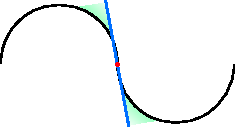
\includegraphics[scale=1.5]{figures/linearizationPoint}
%	\caption{Sketch of linearization for the Cubli frame angels.}
%	\label{LinearizationSketch}
%\end{figure} 
%
%Due to the linearization of the model there will be an point where the controller will no longer be able to catch the frame, because the linear model does not work anymore. In the sketch (see \figref{LinearizationSketch}) the area of operation for the controller is indicated by the green area.    %-------- Linearization
	\section{Block Diagram}

To verify the model in simulation \eqref{FrameEq4TaylerApprox} is transformed into the Laplace domain, after which a transfer function of the system is derived. The proceeding equations are valid only around the operating point, and so for better overview, in the following \si{\Delta \theta_F = \theta_F}.
%
\begin{flalign}
	\eq{(J_F+m_w \cdot {l_w}^{2}) \cdot \theta_F \cdot s^2}{-B_F \theta_F\cdot s +  ( m_F \cdot l_F + m_w \cdot l_w ) g \cdot \theta_F - \tau_m + B_w \theta_w\cdot s } & \nonumber\\
\label{LaplaceOfLinearizedModel}
\end{flalign}
%
The angle of the reaction wheel, \si{\theta_w}, still features in \eqref{LaplaceOfLinearizedModel}. It is desirable to have only one input, \si{\tau_m}, and one output, \si{\theta_F}. To achieve this, \eqref{WheelRotEq2} is transformed into the Laplace domain and solved for \si{\theta_w}.
%
\begin{flalign}
	\eq{\theta_w\cdot s^2} {\frac{\tau_m - B_w \theta_w\cdot s}{J_w} - \theta_F\cdot s^2}   &\\
	\eq{\theta_w} {\frac{ -J_w \theta_F \cdot s^2 + \tau_m }{ J_w \cdot s^2 + B_w \cdot s }}&
\label{WheelRotEq2Laplace}
\end{flalign}
%
\Eqref{WheelRotEq2Laplace} is now substituted for \si{\theta_w} in \eqref{LaplaceOfLinearizedModel}, and the transfer function is of the system is derived.
%
\begin{flalign}
	\eqOne{(J_F+m_w \cdot {l_w}^{2}) \cdot \theta_F \cdot s^2}{-B_F \theta_F\cdot s +  ( m_F \cdot l_F + m_w \cdot l_w ) g \cdot \theta_F - \tau_m}
	\eqTwo{+ B_w ( \frac{ -J_w \theta_F \cdot s^2 + \tau_m }{ J_w \cdot s^2 + B_w \cdot s } )\cdot s }&\nonumber
\label{CubliTransferFunction}
\end{flalign}

\vspace{-.2cm}
\large{\si{\frac{\theta_F}{\tau_m} =}}\nolinebreak
\Large{
\si{\frac{\frac{s}{-J_F - m_w \cdot {l_w}^2}}{s^3 + \left( \frac{B_w}{J_w} + \frac{B_w + B_F}{J_F + m_w \cdot {l_w}^2} \right) s^2 - \left( \frac{ \left( m_F \cdot l_F + m_w \cdot l_w \right)\cdot g}{ \left( J_F + m_w \cdot {l_w}^2 \right) J_w} - \frac{B_F B_w}{ \left(J_F + m_w \cdot {l_w}^2 \right) J_w} \right) s - \frac{\left(m_F \cdot l_F + m_w \cdot l_w \right) B_w\cdot g}{\left(J_F + m_w \cdot {l_w}^2 \right) J_w} }}}\normalsize\vspace{-1.9cm}\\
\vspace{1.8cm}\begin{flalign}\label{2ndCubliTransferFunction}\end{flalign}
%
The transfer function from \eqref{2ndCubliTransferFunction} can be represented as well in the form of a block diagram, as seen in \figref{cubliSimulink}.

% \begin{figure}[H] 
% 	\centering 
% 	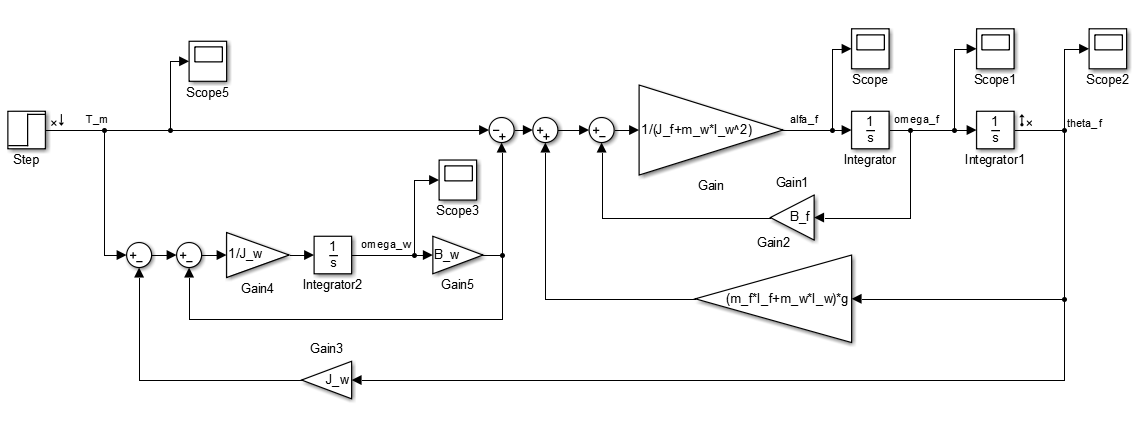
\includegraphics[scale=0.53]{figures/cubliSimulink}
% \end{figure}
% \end{figure} 
\begin{figure}[H]
	  \begin{tikzpicture}[ auto,
                       thick,                         %<--setting line style
                       node distance=1.5cm,             %<--setting default node distance
                       scale=0.75,                     %<--|these two scale the whole thing
                       every node/.style={scale=0.62}, %<  |(always change both)
                       >=triangle 45 ]

    %-- Blocks creation --%
    \draw
      % DIRECT TERM %
      node[shape=coordinate][](input1) at (0,0){}
      node[shape=coordinate][](feedForward) at (0.5,0){}
      node(sum1) at (7.75,0) [sum] {$\sum$}
      node(sum2) at (9.25,0) [sum]{$\sum$}
      node(sum3) at (10.75,0) [sum]{$\sum$}

      node(torque2rotacc1) at (12.85,0) [block]{\Large $\frac{1}{J_F + m_w \cdot {l_w}^{2}}$}

      node(integration1) at (15.75,0) [block] {\Large $\frac{1}{s}$}
      node(integration2) at (18.2,0) [block] {\Large $\frac{1}{s}$}

      node[shape=coordinate][](output) at (19,0){}
      node[shape=coordinate][](veloFeedbackNode) at (16.8,0){}
      node[shape=coordinate][](accFeedbackNode) at (14.5,0){}
    ;
    \draw
      % REACTION WHEEL EQUATIONS %  
      node(sum4) at (1.5,-2) [sum]{$\sum$}
      node(sum5) at (2.85,-2) [sum]{$\sum$}

      node(torque2rotacc2) at (4.3,-2) [block]{\Large $\frac{1}{J_w \cdot s}$}
      % node(integration3) [block, right of = torque2rotacc2] {$\frac{1}{s}$}
      node(frictionWheel) at (6.9,-2) [block] {\Large $B_w$}

      node[shape=coordinate][](veloWheelFeedback) at (7.75,-3.5){}
    ;
    \draw
      % FEEDBACKS %
      node(accFeedback) at (4, -6) [block] {\Large $J_w$}
      node(veloFeedback) at (12.65,-2) [block] {\Large $B_F$}
      node(angleFeedback) at (11.65,-4) [block] {\Large $(m_F \cdot l_F + m_w \cdot l_w)g$}
    ;
    %-- Block linking --%
    % INPUT %
    \draw[-](input1)        -- node{\Large $\tau_m(s)$}(feedForward);
    \draw[->](feedForward)  -- (sum1);

    % OUTPUT %
    \draw[-](integration2)  -- (output);
    \draw[->](output)       -- node {\Large $\theta_{F}(s)$} (20,0);

    % DIRECT TERM %
    \draw[->] (sum1)            -- (sum2);
    \draw[->] (sum2)            -- (sum3);
    \draw[->] (sum3)            -- (torque2rotacc1);
    \draw[->] (torque2rotacc1)  -- node{\Large $\alpha_F(s)$}(integration1);
    \draw[->] (integration1)    -- node{\Large $\omega_F(s)$}(integration2);

    % REACTION WHEEL EQUATIONS %
    \draw[->] (feedForward)     |- (sum4);
    \draw[->] (sum4)            -- (sum5);
    \draw[->] (sum5)            -- (torque2rotacc2);
    \draw[->] (torque2rotacc2)  -- node{\Large $\omega_w(s)$}(frictionWheel);
    % \draw[->] (integration3)    -- (frictionWheel);
    \draw[->] (frictionWheel)   -| (sum1);

    \draw[-] (frictionWheel)       -| (veloWheelFeedback);
    \draw[->] (veloWheelFeedback)  -| (sum5);

    % FEEDBACKS
    \draw[->] (accFeedbackNode)  |- (accFeedback);
    \draw[->] (accFeedback)      -| (sum4);

    \draw[->] (output)           |- (angleFeedback);
    \draw[->] (angleFeedback)    -| (sum2);

    \draw[->] (veloFeedbackNode) |- (veloFeedback);
    \draw[->] (veloFeedback)     -| (sum3);

    %-- Nodes --%
    \draw%--------------------------------------------------------------
      node at (input1)            [shift={(-0.04, -0.05 )}] {\Large \textopenbullet}
      node at (output)            [shift={( 0.007, -0.05 )}] {\Large \textbullet}
      node at (veloFeedbackNode)  [shift={( 0.007, -0.05 )}] {\Large \textbullet}
      node at (accFeedbackNode)   [shift={( 0.007, -0.05 )}] {\Large \textbullet}
      node at (feedForward)       [shift={( 0.007, -0.05 )}] {\Large \textbullet}
      node at (frictionWheel)     [shift={( 1.025, -0.04 )}] {\Large \textbullet}
    ;

    %-- Summation signs --%
      \draw%--------------------------------------------------------------
      node at (sum1) [right = -6.6mm, below = .6mm] {$-$}
      node at (sum1) [right = -3mm, below = 3.9mm]  {$+$} 
      node at (sum2) [right = -6.6mm, below = .6mm] {$+$}
      node at (sum2) [right = -3mm, below = 3.9mm]  {$+$}
      node at (sum3) [right = -6.6mm, below = .6mm] {$+$}
      node at (sum3) [right = -3mm, below = 3.9mm]  {$-$}
      node at (sum4) [right = -6.6mm, below = .6mm] {$+$}
      node at (sum4) [right = -3mm, below = 3.9mm]  {$-$}
      node at (sum5) [right = -6.6mm, below = .6mm] {$+$}
      node at (sum5) [right = -3mm, below = 3.9mm]  {$-$}
    ;

  \end{tikzpicture}
	\caption{Block diagram of the system}
	\label{cubliSimulink}
\end{figure}

    		    %-------- Block Diagram
	
	%---------- Chapter 6 ---------------------------------------- Plant Analysis
	\chapter{Requirements}\label{chap:requirements}
	\section{Acquisition of Parameters}\label{sec:Param}

A method to obtain the parameters from the wheel (mass, distance from its center to the pivoting point of the frame, inertia with respect to its center of rotation and friction) is provided in \appref{app:wheelParameters}. However, as these parameters should remain constant and they have been obtained by previous project runners, it is chosen to use these known parameters\cite{SVJohansen}.

\begin{table}[H]
	\centering
	\begin{tabular}{|l|l|p{3cm}|}
		\hline %-----------------------------------------------------------------------------------
		\textbf{Parameter} &\textbf{Value} &\textbf{Units}\\
		\hline %-----------------------------------------------------------------------------------
		\si{m_w}         & \si{0,222}       &kg\\
		\hline
		%-----------------------------------------------------------------------------------
		\si{l_w}         & \si{0,093}       &m\\
		\hline %-----------------------------------------------------------------------------------
		\si{J_w}         & \si{0,601 \cdot 10^{-3}}	&\si{kg \cdot m^2}\\
		\hline  
		%-----------------------------------------------------------------------------------
		\si{B_w}         & \si{17,03 \cdot 10^{-6}}       &N \si{\cdot m \cdot s \cdot rad^{-1}}\\
		\hline
	\end{tabular}
	\caption{Parameters of the wheel.}
	\label{ParametersWheel}
\end{table}
%

In the previous sections parameters have been found, however, some critical parameters were given from a previous project. When these parameters were found, the Cubli had another mass, due to some physical modifications of the platform, which were performed after the referred project.

\subsection{Mass of the Frame}
The first one to find is the mass of the frame, which can be measured by weighing the setup without the base and substracting the known mass of the wheel. This gives a mass of \si{0,548\ kg}, see \appref{app:MassFrameCenterOfMass}.

\subsection{Center of Mass of the Frame}
The new center of mass can be found hanging the frame from different corners and measuring the deviation angle from the vertical position in every direction. This gives a center of mass which can be seen in \figref{centerOfMassDiagram}. 
\begin{figure}[H]
	\centering
	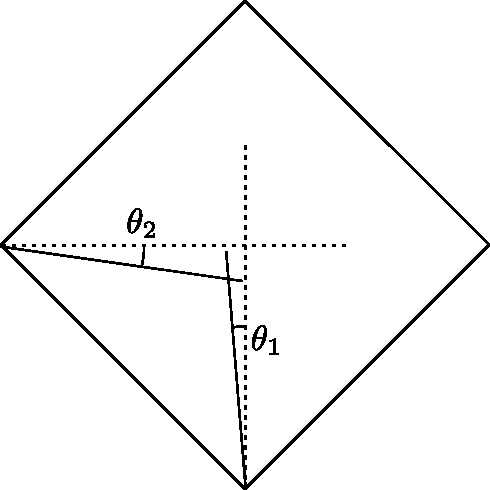
\includegraphics[scale=0.6]{figures/centerOfMassDiagram}
	\caption{Location of the center of mass, where \si{\theta_1=0,043\ rad\ and\ \theta_2=0,078\ rad}.}
	\label{centerOfMassDiagram}
\end{figure}

The new point is not in the vertical line as it was assumed in the model, but this can be solved correcting the offset in the calculation of the angle inside the control loop and taking this new point as the equilibrium one. 

The new \si{l_F} can then be obtained projecting the center of mass onto the vertical line, resulting in \si{8,498\ cm},\appref{app:MassFrameCenterOfMass}.

\subsection{Inertia and Friction of the Frame}
The last parameters, \si{J_F} and \si{B_F}, can not be measured directly so they have to be estimated. The starting point is given by the parameters from the previous report, as seen on \figref{InitialModelParameterCompare}. 

\begin{figure}[H] 
	\centering
	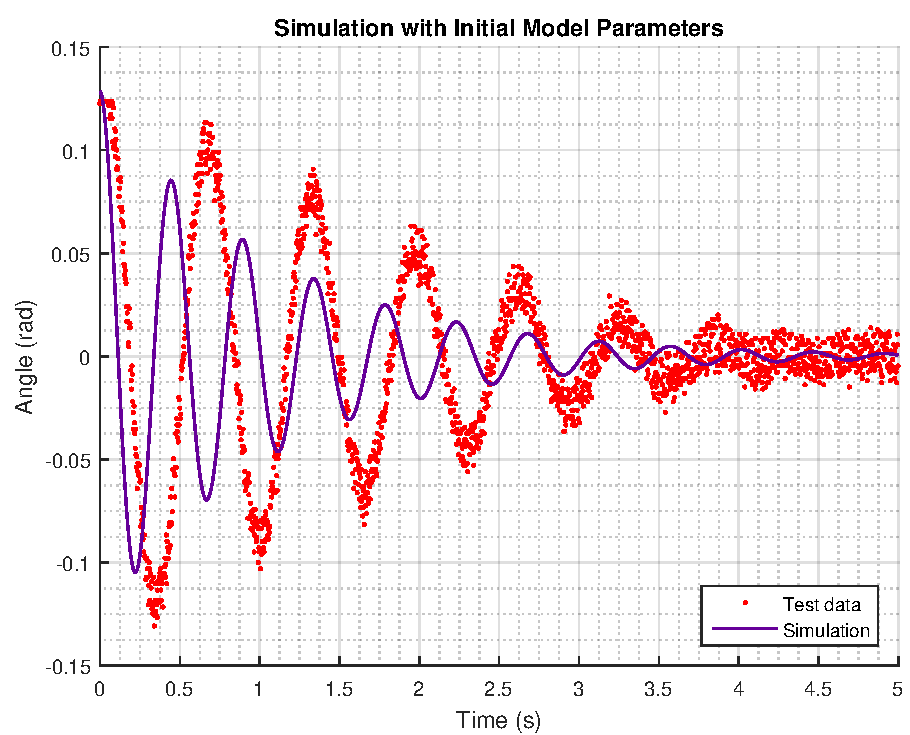
\includegraphics[width=.6\textwidth]{figures/InitialModelParameterCompare}
	\caption{A comparison of the model simulation and the initially given parameters (\si{J_F=6,08 \cdot 10^{-3}\ kg \cdot m^2\ and\ B_F=5,32 \cdot 10^{-3}\ m \cdot s \cdot rad^{-1}}). Data is obtained through \appref{app:impulseResponseAppendix}.}
	\label{InitialModelParameterCompare}
\end{figure}
%
This problem can be solved using optimization, which is the subject of the proceeding section.  	    %-------- Parameter Estimation
	\section{Parameter Estimation using Optimization}
In this section two methods for optimization will be investigated. The base of the implementation is in this case a Matlab script which is fed with test data along with the model simulation, whose task is to fit the model output to the test data by adjusting one or more parameters in the model. In this case the model representation supplied to the script is a Simulink model, which can then be run by the script whenever needed and the script can modify the parameters to be adjusted. The process is iterative in most cases.

\subsection{The Optimization Problem}
The basic scheme for the optimization problem is given in \figref{SensToolSchema}.
%
\begin{figure}[H]
	\centering
	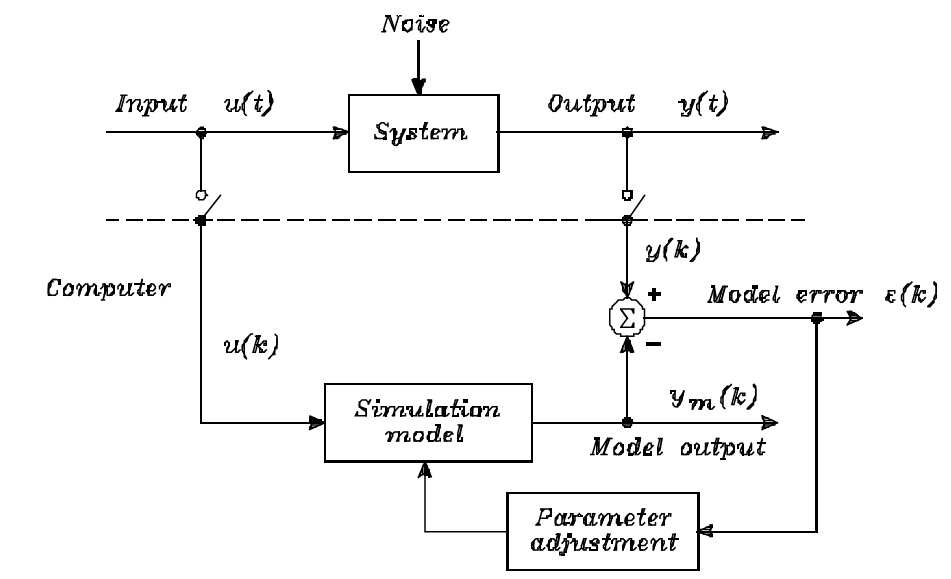
\includegraphics[scale=0.4]{figures/SensToolSchema}
	\caption{Schematic of the optimization problem}
	\label{SensToolSchema}
\end{figure}
%
The provided data is taken from an initial value test of the Cubli hanging down like a pendulum, see \appref{impulseResponseAppendix}.
As the operating angle goes from \si{-0,15\ to\ 0,15\ rad}, the behavior at this range will be better if the fit is done between this operating points. 

Furthermore, the nonlinear model is used to accurately describe the oscillatory behavior of the pendulum. The model is modified such that it describes the system as a regular pendulum without the dynamics of the reaction wheel, in order to match the test conditions under which the data was extracted, as seen in \figref{blockDiagramSenseTool},
%
\begin{figure}[H]
	  \begin{tikzpicture}[ auto,
                       thick,                         %<--setting line style
                       node distance=1.5cm,             %<--setting default node distance
                       scale=0.75,                     %<--|these two scale the whole thing
                       every node/.style={scale=0.62}, %<  |(always change both)
                       >/.tip={Triangle[angle=40:5pt]}
                       ]

    %-- Blocks creation --%
    \draw
      % DIRECT TERM %
      node[shape=coordinate][](input1) at (0,0){}
      node[shape=coordinate][](feedForward) at (0.5,0){}
      node(sum1) at (2.25,0) [sum]{\si{\sum}}
      node(sum2) at (3.75,0) [sum]{\si{\sum}}

      node(torque2rotacc1) at (6.85,0) [block]{\large \si{\frac{1}{J_F + J_w + m_w \cdot {l_w}^{2}}}}

      node(integration1) at (10.75,0) [block] {\large \si{\frac{1}{s}}}
      node(integration2) at (14.2,0) [block] {\large \si{\frac{1}{s}}}

      node[shape=coordinate][](output) at (15.3,0){}
      node[shape=coordinate][](veloFeedbackNode) at (11.8,0){}
      
    ;
    \draw
      % FEEDBACKS %
      node(veloFeedback) at (7,-2) [block] {\large \si{B_F}}
      node(angleFeedback) at (8,-4) [block] {\large \si{(m_F \cdot l_F + m_w \cdot l_w)g}}
    ;
    %-- Block linking --%
    % INPUT %
    \draw[-](input1)        -- node{\large \si{\tau_m(s)}}(feedForward);
    \draw[->](feedForward)  -- (sum1);

    % OUTPUT %
    \draw[-](integration2)  -- (output);
    \draw[->](output)       -- node {\large \si{\theta_{F}(s)}} (17,0);

    % DIRECT TERM %
    \draw[->] (sum1)            -- (sum2);
    \draw[->] (sum2)            -- (torque2rotacc1);
    \draw[->] (torque2rotacc1)  -- node{\large \si{\alpha_F(s)}}(integration1);
    \draw[->] (integration1)    -- node{\large \si{\omega_F(s)}}(integration2);

    % FEEDBACKS

    \draw[->] (output)           |- (angleFeedback);
    \draw[->] (angleFeedback)    -| (sum1);

    \draw[->] (veloFeedbackNode) |- (veloFeedback);
    \draw[->] (veloFeedback)     -| (sum2);

    %-- Nodes --%
    \draw%--------------------------------------------------------------
      node at (input1)            [shift={(-0.04, -0.05 )}] {\Large \textopenbullet}
      node at (output)            [shift={( 0.007, -0.05 )}] {\Large \textbullet}
      node at (veloFeedbackNode)  [shift={( 0.007, -0.05 )}] {\Large \textbullet}
    ;

    %-- Summation signs --%
      \draw%--------------------------------------------------------------

      node at (sum1) [right = -6.6mm, below = .6mm] {$-$}
      node at (sum1) [right = -3mm, below = 3.9mm]  {$+$}
      node at (sum2) [right = -6.6mm, below = .6mm] {$+$}
      node at (sum2) [right = -3mm, below = 3.9mm]  {$-$}

    ;

  \end{tikzpicture}
	\centering
	\caption{Block diagram of the system}
	\label{blockDiagramSenseTool}
\end{figure}
%
 In order to minimize the difference between the data points measured in test and the output of the model, a function to describe such a relationship is needed. The performance function used to describe goodness of the fit, is a mean square error function.
%
\begin{flalign}
	\eq{\vec{P}(\vec{\theta})} {\frac{1}{2N}\sum_{k = 1}^{N} \left(\vec{y}(kT) - \vec{y_m}(kT, \vec{\theta})\right)^2 } &
\label{performanceFunction}
\end{flalign}
%
\hspace{6mm} Where:\\
\begin{tabular}{ p{1cm} l l l}
& \si{\vec{\theta}}   & is the parameter(s) to be adjusted                  & \\
& \si{N}              & is the degrees of freedom for each parameter        & \\
& \si{k}              & is the sample indexes, \si{k=1,\ 2,} ...\si{,\ N}   & \\
& \si{T}              & is the sampling time                                & \\
& \si{\vec{y}}        & is the test measurement output vector               & \\
& \si{\vec{y_m}}      & is the model output vector                          & \\
\end{tabular}

A normal mean square error function is only divided by the degrees of freedom, \si{N}, but in tis case is divided by \si{2N} to cancel out the factor which arises when computing its gradient. This only gives the function a constant offset and does not have any impact when minimizing it.

\subsection{Steepest Descent Method}
One way of solving the optimization problem is through the use of the gradient. It indicates in which direction the steepest descent (or ascent) is found in an infinitesimal surrounding of a given starting point.

For a function \si{f(x)} with a change in \si{x} of \si{\delta}, the following can be obtained from the Taylor series.
%
\begin{flalign}
  f(x) + \Delta f(x) = f(\vec{x}+\vec{\delta}) &\approx f(x) + \vec{g}^T \vec{\delta} + \frac{1}{2} \vec{\delta}^T \vec{H}\vec{\delta} &
\label{taylorApproximation}
\end{flalign}
%
\hspace{6mm} Where:\\
\begin{tabular}{ p{1cm} l l l}
& \si{\vec{g}} 					    	   & is the gradient \si{\nabla f(x)}     & \\
& \si{\vec{H}} 					    	   & is the Hessian                       & \\
& \si{\vec{\delta}} 					   & is the change in \si{x}              & \\
\end{tabular}

%Then the change in \si{f(x)} as \si{||\vec{\delta}||_2 \rightarrow 0} can be approximated as follows.
%%
%\begin{flalign}
%  \Delta f(x) &\approx \vec{g}^T \vec{\delta} = ||\vec{g}||_2 \ ||\vec{\delta}||_2 \ cos \theta &
%\label{changeInF}
%\end{flalign}
%%
%\hspace{6mm} Where:\\
%\begin{tabular}{ p{1cm} l l l}
%& \si{\theta} 					    	   & is the angle between \si{\vec{g}} and \si{\vec{\delta}}     & \\
%\end{tabular}

In steepest descend method only the first order Taylor approximation is used, that is, the last term, \si{\frac{1}{2} \vec{\delta}^T \vec{H}\vec{\delta}} is discarded. If the derivative of the first order approximation is set to zero, the following is obtained.
%
\begin{flalign}
  \frac{\partial}{\partial \vec{\delta}} \ f(\vec{x}+\vec{\delta}) &\approx \vec{g} = 0 &
\label{1stOrderTaylorApproximationParThetaEqZero}
\end{flalign}

That is, if the gradient of the function to be minimized is 0, a minimum or maximum exists as a candidate for a solution in this point. It follows that if standing in some point and computing the gradient in this point, then the gradient, \si{\vec{g}}, is the steepest ascend and the negative gradient, \si{-\vec{g}}, is the steepest descend. This only takes into account the immediate surroundings of the initially chosen point. A visualization of how the negative gradient points to a minimum of an arbitrary function is seen in \figref{visualizationOfGradient}.

\begin{figure}[H] 
	\centering
	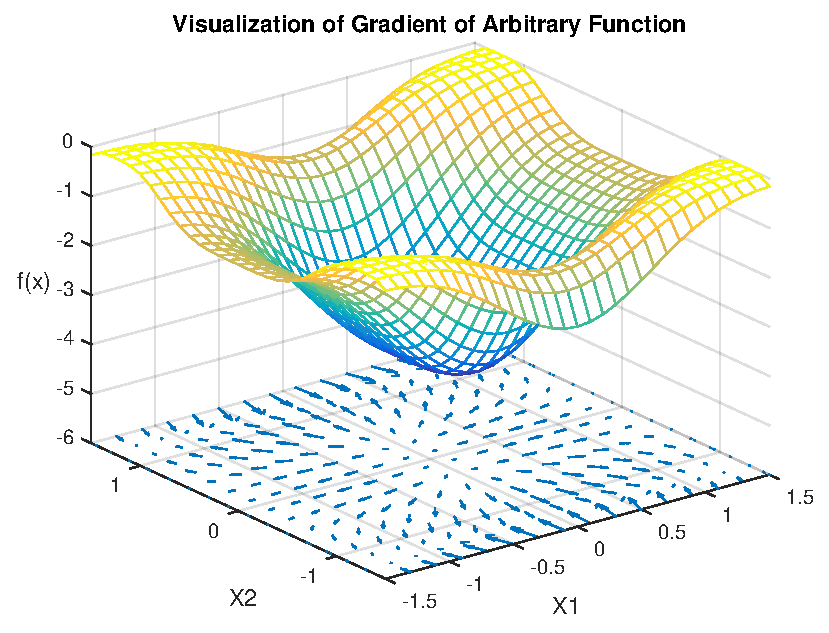
\includegraphics[width=.8\textwidth]{figures/visualizationOfGradient}
	\caption{Visualization of gradient of an arbitrary function.}
	\label{visualizationOfGradient}
\end{figure}

One way of implementation is to set a step-size which decides how far in the \si{-\vec{g}} direction to go. The step-size can then be scaled in each iteration to avoid taking too large steps as shown in \figref{SteepestDescendLargeStep} and \ref{SteepestDescendSmallStep}, where \si{s^*} is the value of \si{x} which minimizes \si{f(x)}, \si{x_0} is the starting point at which \si{-\vec{g}} is computed and \si{x} is the point reached after the step.
%
\begin{minipage}{\linewidth}
	\begin{minipage}{0.45\linewidth}
		\begin{figure}[H]
			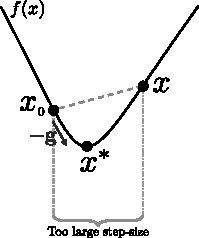
\includegraphics[scale=1.4]{figures/gradientDescendLargeStep}
			\centering
			\captionsetup{justification=centering}
			\captionof{figure}{A too large step will cause the algorithm to step over the valley, resulting in a larger value of f(x) in the \si{-\vec{g}} direction}
			\label{SteepestDescendLargeStep}
		\end{figure}
	\end{minipage}
	\hspace{0.03\linewidth}
	\begin{minipage}{0.45\linewidth}
		\begin{figure}[H]
			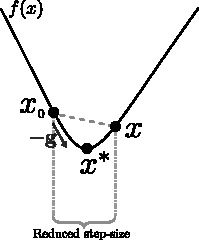
\includegraphics[scale=1.4]{figures/gradientDescendReducedStep}
			\centering
			\captionsetup{justification=centering}
			\captionof{figure}{By going back and choosing a smaller step, a smaller value for f(x) is obtained}
			\label{SteepestDescendSmallStep}
		\end{figure}
	\end{minipage}
\end{minipage}

The steepest descend method does find a minimum. However, it converges to it rather slowly. An implementation where it is possible to directly retrieve the gradient of the function which is to be minimized, \si{f(x)}, is shown in \figref{steepestDescendEx}.

\begin{minipage}{\linewidth}
	\begin{minipage}{0.45\linewidth}
		\begin{figure}[H]
			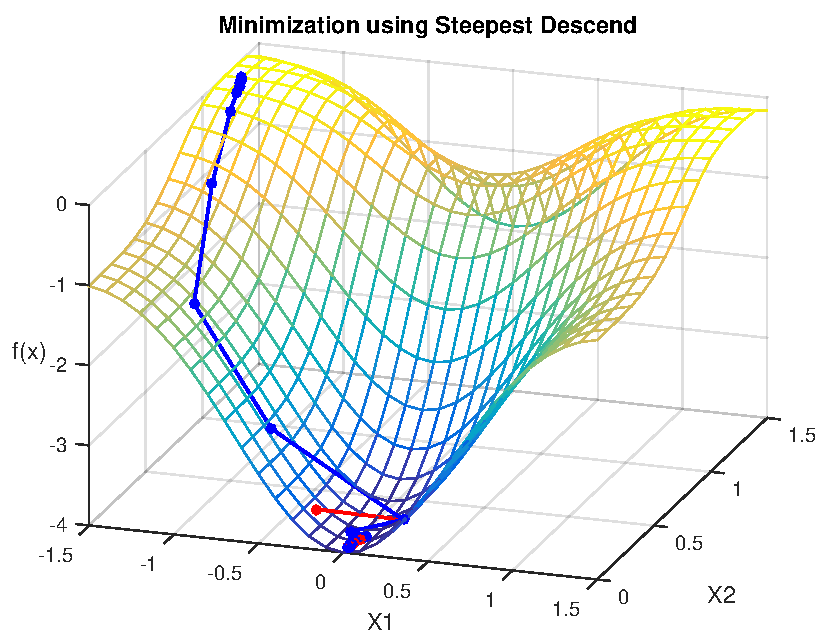
\includegraphics[scale=.6]{figures/steepestDescendEx}
			\centering
			\captionsetup{justification=centering}
			\captionof{figure}{An example of a direct implementation of the steepest descend method. It steps over the valley and the step size is reduced in the red iteration}
			\label{steepestDescendEx}
		\end{figure}
	\end{minipage}
	\hspace{0.03\linewidth}
	\begin{minipage}{0.45\linewidth}
		\begin{figure}[H]
			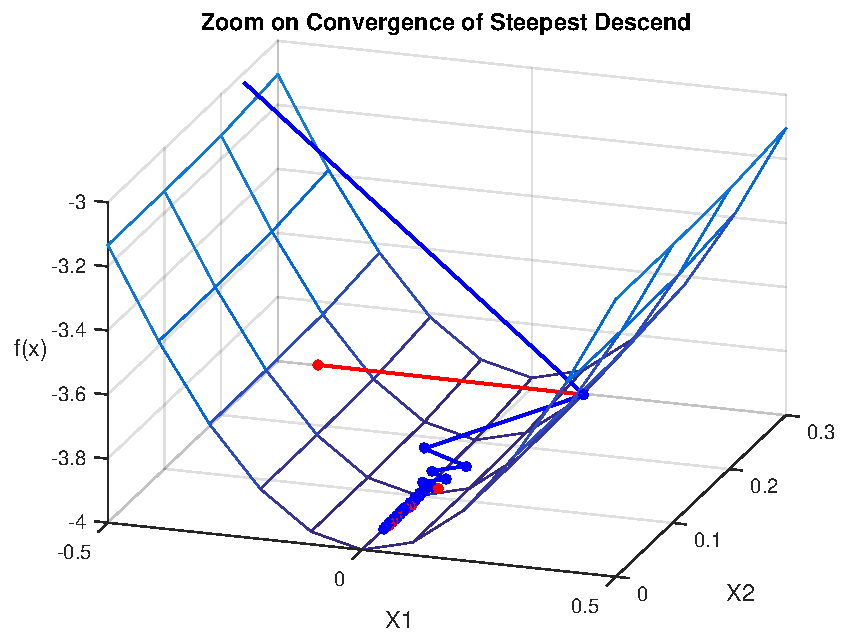
\includegraphics[scale=.6]{figures/steepestDesendExZoom}
			\centering
			\captionsetup{justification=centering}
			\captionof{figure}{From the zoom on the convergence, it can be seen that many iterations (here 100) are needed using this method}
			\label{steepestDesendExZoom}
		\end{figure}
	\end{minipage}
\end{minipage}

%From the zoom on \figref{steepestDesendExZoom} the convergence toward %the minimum is clear, however it is also clear that many iterations are %needed to get there.

\subsection{Newton's Method}
Another approach is called Newton's Method, which is also rooted in the Taylor approximation. However, this method also uses the second order term of the approximation.
%
\begin{flalign}
  f(x) + \Delta f(x) = f(\vec{x}+\vec{\delta}) &\approx f(x) + \vec{g}^T \vec{\delta} + \frac{1}{2} \vec{\delta}^T \vec{H}\vec{\delta} &
\label{taylorApproximation2ndOrder}
\end{flalign}

In this case the derivative of the approximation is set to 0, and the following is obtained.
%
\begin{flalign}
  \frac{\partial}{\partial \vec{\delta}} \ f(\vec{x}+\vec{\delta}) &\approx \vec{g} + \frac{1}{2}\ \frac{\partial}{\partial \vec{\delta}}\ \vec{H}\vec{\delta}^2 &\\
  \frac{\partial}{\partial \vec{\delta}} \ f(\vec{x}+\vec{\delta}) &\approx \vec{g} + \vec{H}\vec{\delta} = 0 &
\label{2stOrderTaylorApproximationParThetaEqZero}
\end{flalign}

Using this to find an expression for the difference in \si{x}, \si{\vec{\delta}}, yields the following.
%
\begin{flalign}
  0 &= \vec{g} + \vec{H}\vec{\delta}  &\\
  \vec{\delta} &= -\vec{H}^{-1}\vec{g} &
\label{NewtonsMethod}
\end{flalign}

This expression can then be used to choose the value of \si{\vec{\delta}} such that \si{f(x)} is minimized. An implementation where it is possible to directly retrieve the gradient and a Hessian of the function which is to be minimized, \si{f(x)}, is shown in \figref{NewtonsMethodEx}. 
%
\begin{figure}[H] 
	\centering
	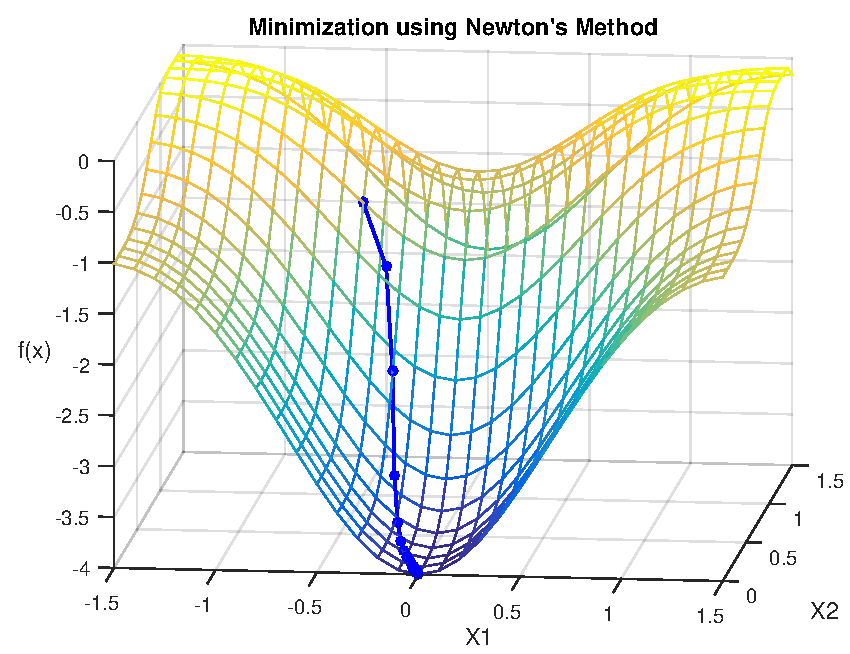
\includegraphics[width=.7\textwidth]{figures/NewtonsMethodEx}
	\caption{Example of a direct implementation of Newton's method for optimization.}
	\label{NewtonsMethodEx}
\end{figure}

If compared to the steepest descend method in \figref{steepestDescendEx} and \ref{steepestDesendExZoom}, where 100 iterations were used, it is clear how Newton's method converges much faster, in 30 iterations, to the minimum of \si{f(x)}. 

\subsection{Implementation of Newton's Method}
When implementing Newton's Method both the gradient and the Hessian of the performance function \eqref{performanceFunction} are needed.
%
\begin{flalign}
	\frac{\partial \vec{P}(\vec{\theta}) }{\partial \vec{\theta}} &= G(\vec{\theta}) = \frac{\partial}{\partial \vec{\theta}} \left( \frac{1}{2N}\sum_{k = 1}^{N} \left(\vec{y}(kT) - \vec{y_m}(kT, \vec{\theta})\right)^2 \right) &\\
  \eq{\vec{G}(\vec{\theta})} {- \frac{1}{N}\sum_{k = 1}^{N} \left((\vec{y}(kT) - \vec{y_m}(kT, \vec{\theta})) \ \frac{\partial  \vec{y_m}(kT, \vec{\theta})}{\partial \vec{\theta}} \right) } &
\label{gradientOfPerformanceFunction}
\end{flalign}

Since the Matlab implementation uses a Simulink model the problematic part of \eqref{gradientOfPerformanceFunction} is the derivative of the model with respect to the model parameters, \si{\frac{\partial  \vec{y_m}(kT, \vec{\theta})}{\partial \vec{\theta}}}. To solve this problem a numerical differentiation of the model is applied as shown in \autoref{AlgorithmForNummericalDiff}.

\begin{lstlisting}[ language = Matlab,
                    caption  = {Algorithm for numerical differentiation of the simulated model},
                    label    = AlgorithmForNummericalDiff ]

  %small deviation from parameters, J_f and B_f, is set
  p = 0.001;
  
  %calculating the deviation
  deltaJ_f = p*J_f; deltaB_f = p*B_f;
  
  %saving the old parameters:
  J_f_old = J_f; B_f_old = B_f;
  
  %setting deviating parameters ready for simulation
  J_f = deltaJ_f;
  
  %running the simulation again, now with deviation in J_f
  sim('CubliParameterEstimation.slx');
  
  %storring the result of the simulation
  deltaYmJf = simOut;
  
  %setting deviating parameters ready for simulation
  B_f = deltaB_f; J_f = J_f_old; %<--restoring J_f
  
  %running the simulation again, now with deviation in B_f
  sim('CubliParameterEstimation.slx');
  
  %storring the result of the simulation
  deltaYmBf = simOut;
  
  %restoring the parameters to their original value
  B_f = B_f_old;
  
  %calculating the derivatives of the model
  YmDiffBf = ( deltaYmBf - Ym )/ p;
  YmDiffJf = ( deltaYmJf - Ym )/ p;
\end{lstlisting}

Now that the model partial derivatives are found, all parts of the gradient, as represented in \eqref{gradientOfPerformanceFunction}, are known. The Hessian is also needed and can be represented as,
%
\begin{flalign}
	\vec{H}(\vec{\theta}) &= \frac{\partial^2 \vec{P}(\vec{\theta}) }{\partial \vec{\theta}\partial \vec{\theta^T}} = \frac{\partial \vec{G}(\vec{\theta}) }{\partial \vec{\theta}} &
\end{flalign}
%
which leads to the following:
\begin{flalign}
	\vec{H}(\vec{\theta}) &= \frac{1}{N}\sum_{k = 1}^{N} \left(   \frac{\partial  \vec{y_m}(kT, \vec{\theta})}{\partial \vec{\theta}} \left(\frac{\partial \vec{y_m}(kT, \vec{\theta})}{\partial \vec{\theta}} \right)^T  	  - \left(\frac{\partial^2 \vec{P}(\vec{\theta}) }{\partial \vec{\theta}\partial \vec{\theta^T}}\right) (\vec{y}(kT) - \vec{y_m}(kT, \vec{\theta}))  \right) &
\label{hessianOfPerformanceFunction}
\end{flalign}
%
To avoid the second derivative of the performance function in \eqref{hessianOfPerformanceFunction}, the Hessian can be approximated simply by removing this last term.
\begin{flalign}
	\vec{\widetilde{H}}(\vec{\theta}) &\triangleq \frac{1}{N}\sum_{k = 1}^{N} \left(   \frac{\partial  \vec{y_m}(kT, \vec{\theta})}{\partial \vec{\theta}} \left(\frac{\partial \vec{y_m}(kT, \vec{\theta})}{\partial \vec{\theta}} \right)^T \right) &
\label{hessianApproxOfPerformanceFunction}
\end{flalign}
%
This approximation assumes that the model is only linearly dependent on the parameters, \si{\vec{\theta}}. As the error term, \si{(\vec{y}(kT) - \vec{y_m}(kT, \vec{\theta}))}, approaches zero the approximation becomes increasingly accurate.

Running the implementation of Newton's method approximates the model parameters to \si{J_F = } and \si{B_F = }, while giving a normed root mean square error of \si{31.71 \%} as seen on \figref{ParameterEstimationNewtonCubli}. %The normed RMS error is a way to determine the goodness of the fit.

\begin{figure}[H] 
	\centering
	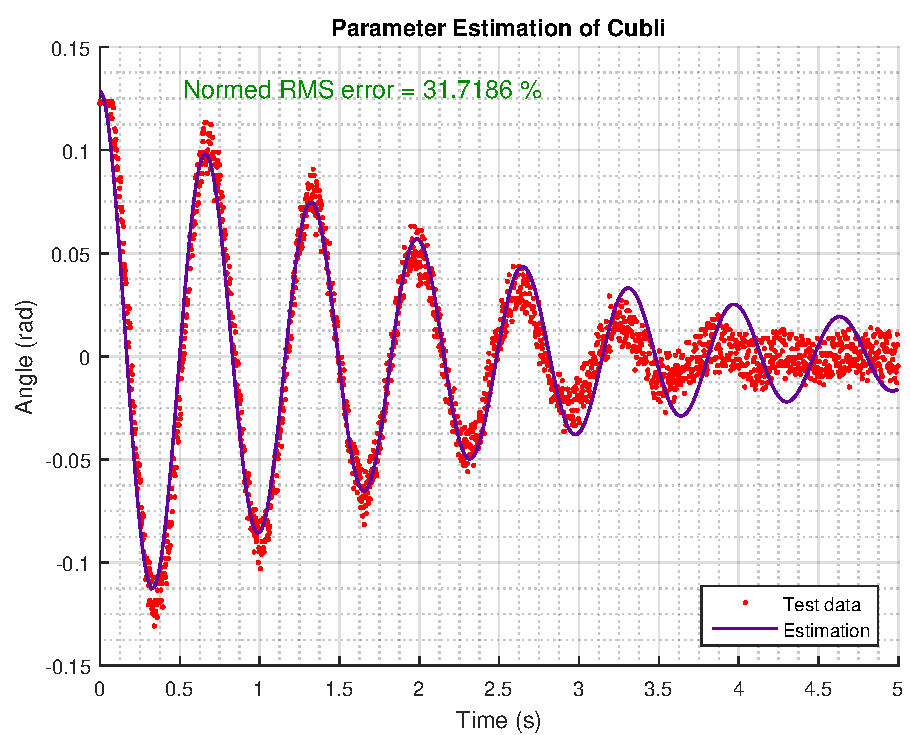
\includegraphics[width=.8\textwidth]{figures/ParameterEstimationNewtonCubli}
	\caption{The result of implementation of Newton's method}
	\label{ParameterEstimationNewtonCubli}
\end{figure}

\subsection{SensTool}
A lot of the background for the implementation above comes from documentation on a Matlab toolbox called SensTool \fxnote{Reference Senstool guide}. The optimization method is implemented in it and it also includes an extra feature based on parameter sensitivity and frequency domain. For a better accuracy on the estimation it is a good decision to use this tool as the final approach to the parameters of the Cubli model.

The same data, Simulink model and initial parameters as the previous case are given to this toolbox and the result of the fit can be seen in \figref{SenseToolParameterEstimation}. 
%
\begin{figure}[H]
	\centering
	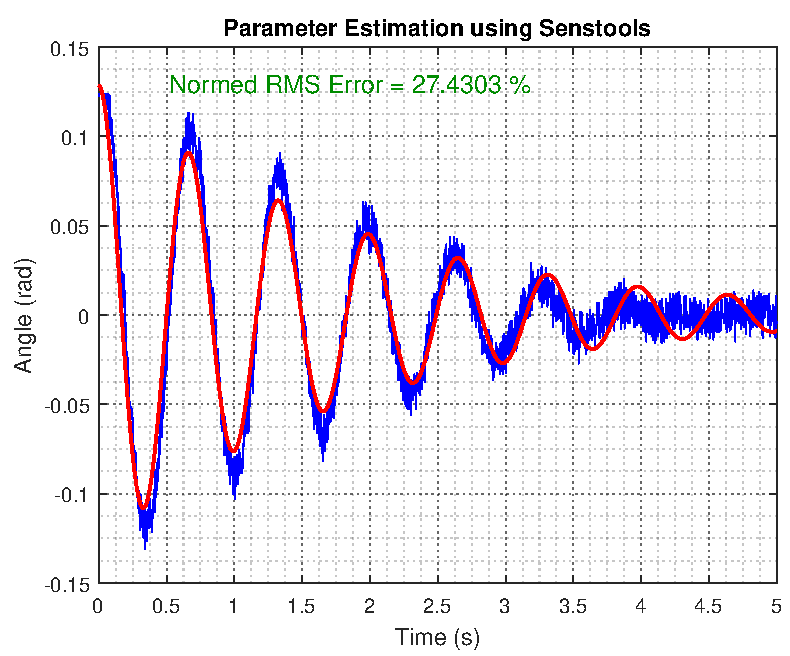
\includegraphics[scale=0.6]{figures/SenseToolParameterEstimation}
	\caption{Data from the test (red) and final fit with the new parameters (blue)}
	\label{SenseToolParameterEstimation}
\end{figure}
%

The final estimated parameters are \si{J_F=4,8 \cdot 10^{-3}\ kg \cdot m^2\ and\ B_F=7,7 \cdot 10^{-3}\ m \cdot s \cdot rad^{-1}}. The normed RMS error is \si{27,4\ \%} compared to the \si{31,7\ \%} shown in \figref{ParameterEstimationNewtonCubli}. The \si{4,3\ \%} error reduction is likely due to additional algorithms.

\section{Final Parameters}
The final parameters of the system can be seen in \ref{ParametersSystem}
\begin{table}[H]
	\begin{tabular}{|l|l|p{3cm}|}
		\hline %-----------------------------------------------------------------------------------
		\textbf{Parameter} &\textbf{Value} &\textbf{Units}\\
		\hline %-----------------------------------------------------------------------------------
		\si{m_w}         & \si{0,222}       &kg\\
		\hline
		%-----------------------------------------------------------------------------------
		\si{l_w}         & \si{0,096}       &m\\
		\hline %-----------------------------------------------------------------------------------
		\si{J_w}            & \si{0,601 \cdot 10^{-3}}	&\si{kg \cdot m^2}\\
		\hline  
		%-----------------------------------------------------------------------------------
		\si{B_w}         & \si{17,03 \cdot 10^{-6}}       &N \si{\cdot m \cdot s \cdot rad^{-1}}\\
		\hline
		%-----------------------------------------------------------------------------------
		\si{m_F}         & \si{0,548}       &kg\\
		\hline
		%-----------------------------------------------------------------------------------
		\si{l_F}         & \si{0,08498}       &m\\
		\hline %-----------------------------------------------------------------------------------
		\si{J_F}            & \si{4,8 \cdot 10^{-3}}	&\si{kg \cdot m^2}\\
		\hline %-----------------------------------------------------------------------------------
		\si{B_F}         & \si{7,7 \cdot 10^{-3}}       &N \si{\cdot m \cdot s \cdot rad^{-1}}\\
		\hline
	\end{tabular}
	\caption{Parameters of the whole system}
	\label{ParametersSystem}
\end{table}             %-------- Optimization and SensTool
	\section{Model testing}
Substituting all the constants of \eqref{2ndCubliTransferFunction} with the parameters of the real model results in the final transfer function of the system.
%
\begin{flalign}
	\eq{G(s)}{\frac{-133 \cdot s}{s^3 + 1,015 \cdot s^2 - 87,74 \cdot s - 2,487}} &\nonumber\\
	\label{RealCubliTransferFunction}	
\end{flalign}
%
Using \eqref{RealCubliTransferFunction} it is possible to simulate the response of the system to a step input and compare it with the response of the simulation of the block diagram. This is done to verify that the block diagram is in fact showing the system described in \eqref{RealCubliTransferFunction}, as seen in \figref{stepComparison}.

\begin{figure}[H] 
	\centering 
	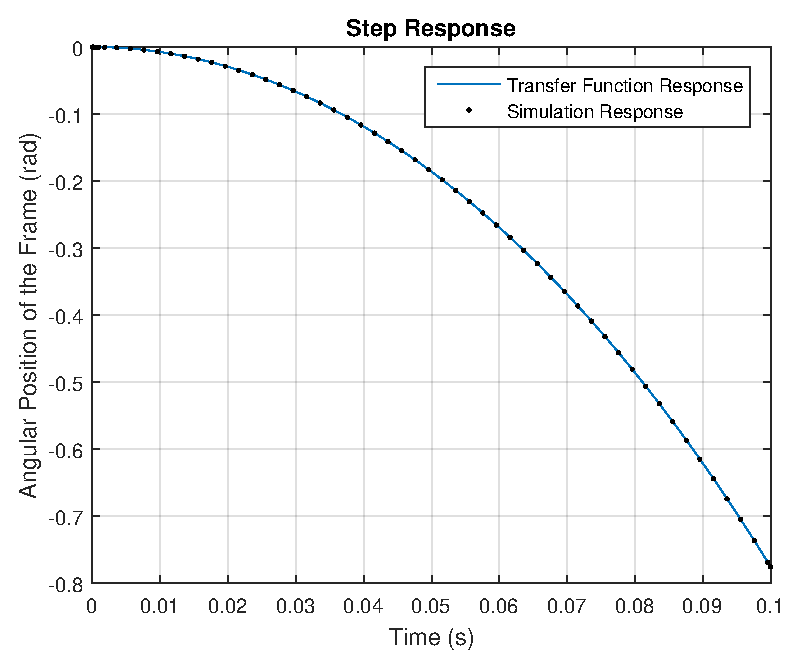
\includegraphics[scale=0.55]{figures/stepComparison}
	\caption{Step response comparison between the transfer function from \eqref{RealCubliTransferFunction} and the block diagram from \figref{cubliSimulink}. The conclusion form this is the blockdiagram of the system was made correctly}
	\label{stepComparison}
\end{figure}


In \figref{LinearizedVSNonlinear}, the effect of the linearization is apparent. In the simulation the frame is placed in upright position very slightly off \si{0\ rad}. The small deviation from \si{0\ rad} is applied in the last plant feedback, see \figref{cubliSimulink}. If, in the simulation, the model is started out at exactly \si{0\ rad}, it will balance in upright position.
\Figref{LinearizedVSNonlinear} shows the behavior around the frame's pivot point and does not include the platform itself. For this reason, the simulation allows for the frame to fall down and act as a normal pendulum. The nonlinear model shows how the pendulum dampens around its natural equilibrium point, while the linear model keeps increasing the angle.
However, in reality the platform blocks the frame's path, and so, it can only ever turn \si{45 ^\circ} to either side, that is, \si{\frac{\pi}{4}\ rad \approx 0,79\ rad}.
%
\begin{minipage}{\linewidth}
  \begin{minipage}{0.5\linewidth}
    \begin{figure}[H]
    	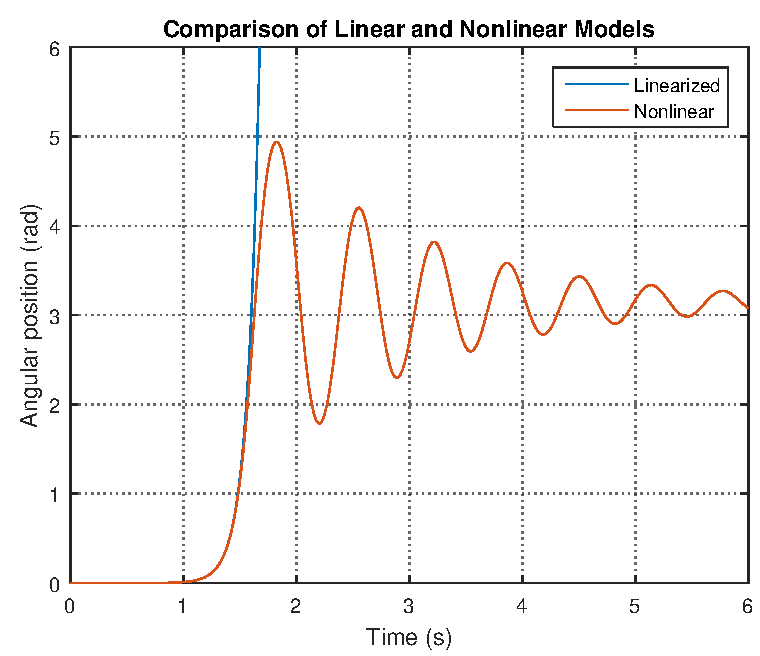
\includegraphics[scale=.5]{figures/LinearizedVSNonlinear}
    	\centering
  		\captionsetup{justification=centering}
  		\captionof{figure}{Simulation of the linearized model compared to the nonlinear model}
  		\label{LinearizedVSNonlinear}
  	\end{figure}
  \end{minipage}
  %	\hspace{0.03\linewidth}
  \begin{minipage}{0.5\linewidth}
  	\begin{figure}[H]%\vspace{4mm}
  		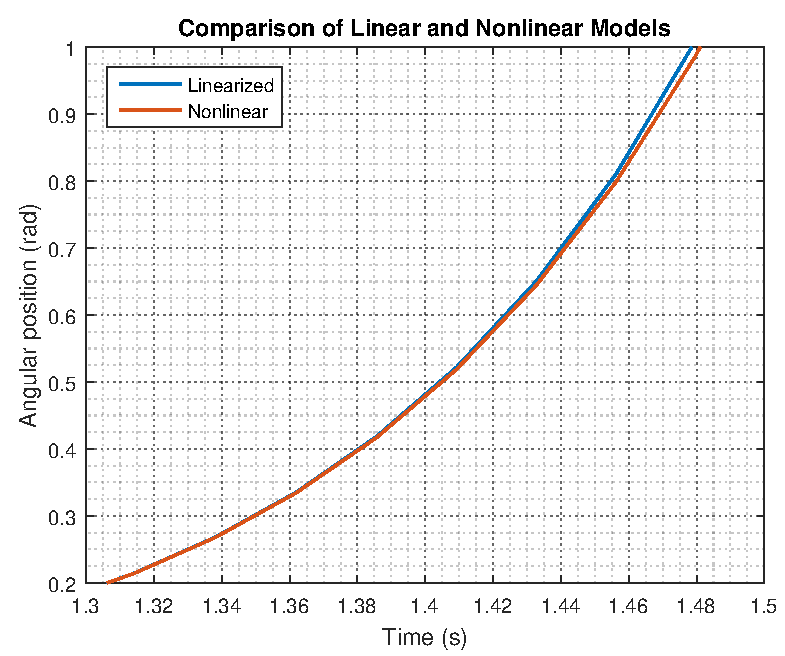
\includegraphics[scale=.5]{figures/LinearizedVSNonlinearZoom}
  		\centering
  		\captionsetup{justification=centering}
  		\captionof{figure}{Zoom of \figref{LinearizedVSNonlinear} from t=1.3s to t=1.5s}
  		\label{LinearizedVSNonlinearZoom}
  	\end{figure}
  \end{minipage}
\end{minipage}

From \figref{LinearizedVSNonlinear} and \figref{LinearizedVSNonlinearZoom}, the linearized model is considered a good approximation of the system's behavior in the operational region of \si{\pm 0,79\ rad}, since the error committed is no more than 0.01 rad at this point.

To further investigate the model, an other test is made, see \appref{fallResponseAppendix}, to determine weather the fall response of the nonlinear model and the real system matches.

\begin{minipage}{\linewidth}
	\begin{minipage}{0.5\linewidth}
		\begin{figure}[H]
			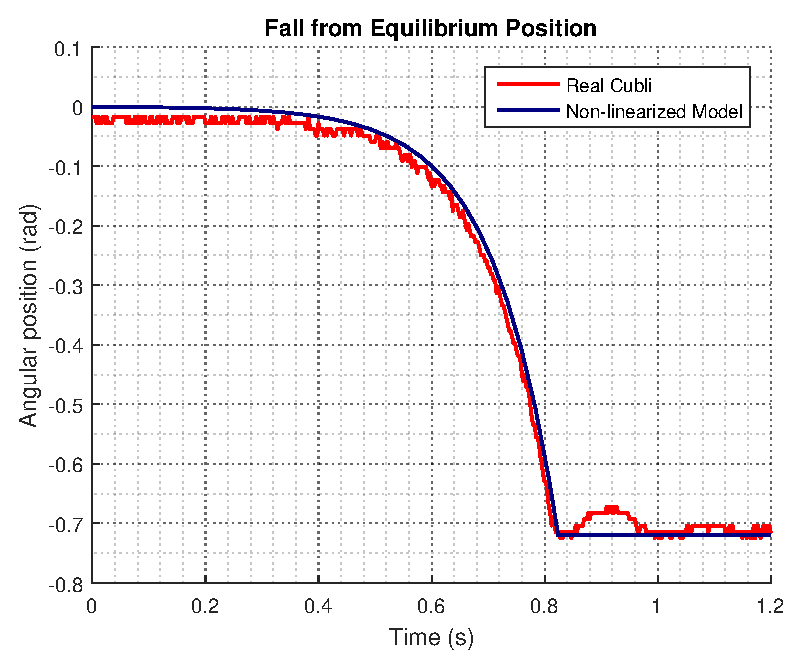
\includegraphics[scale=.48]{figures/FallTestComparison}
			\centering
			\captionsetup{justification=centering}
			\captionof{figure}{Comparison of test and nonlinear model of frame falling from equilibrium position}
			\label{FallTestComparison}
		\end{figure}%\vspace{-5mm}
	\end{minipage}
%	\hspace{0.03\linewidth}
	\begin{minipage}{0.5\linewidth}
		\begin{figure}[H]%\vspace{-4mm}
			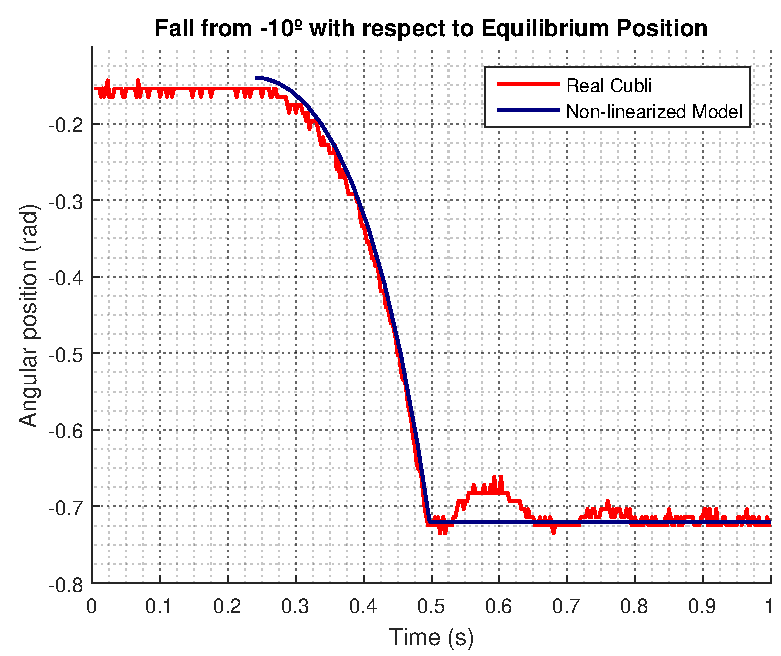
\includegraphics[scale=.48]{figures/FallTestComparison10deg}
			\centering
			\captionsetup{justification=centering}
			\captionof{figure}{Comparison of test and model of frame falling from initial condition \si{-0,174\ rad}}
			\label{FallTestComparison10deg}
		\end{figure}%vspace{-5mm}
	\end{minipage}
\end{minipage}

In \figref{FallTestComparison} the Cubli falls from equilibrium position given a very small impulse. When plotting the two data sets the time of the fall is aligned to see if the characteristics of the simulated fall matches reality.\\
In an attempt to avoid unjustified assumptions the test is repeated from initial condition \si{-0,174\ rad} (\si{-10^\circ}) in both simulation and test, the result is shown in \figref{FallTestComparison10deg}.

%Hence the linearized model is used both for further analysis of the system and for controller design.
		      %-------- Model Analysis
	\section{Stability Analysis}\label{sec:stabilityAnalysis}
The linearized model is considered valid within the discussed range of angles (\si{\pm 0,79\ rad}), so it can be used to do a deeper analysis on the behavior of the system. %This includes evaluations in frequency domain, s-domain and L(s)-domain.

%\subsection{Bode Diagram}
%The Bode diagram gives the frequency response of the system, in both magnitude and phase plots, as seen in \figref{bodeTF}.
%\begin{figure}[H] 
%	\centering 
%	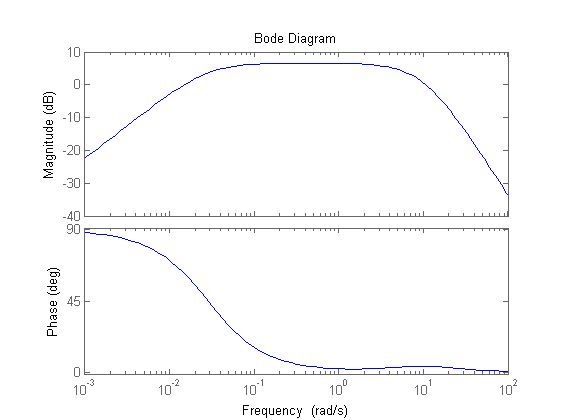
\includegraphics[scale=0.65]{figures/bodeTF}
%	\caption{Bode diagram of the system}
%	\label{bodeTF}
%\end{figure} 
%
%The graph also provides information about the stability of the system, given by the gain and phase margins. 
%
%In this case the first one is just infinite because the phase never crosses \si{-180^o} or \si{180^o}. However, the phase margin is \si{-118^o}, which means that the phase has some margin before becoming unstable.
%
%Looking only at the Bode plot, the system may be seen as stable, but the inverted pendulum is known to be an unstable system, so further analysis has to be done.

\subsection{Root Locus}
The Root Locus plot gives information about the location of the poles and zeros in open loop, and how the poles in closed loop will change as the gain of the whole system increases.

As seen in \figref{rlocusCubli} and \figref{rlocusCubliZoom} the system has one zero \si{(s=0)}, and three poles \si{(s=-10,5014}, \si{s=-0,0283} and \si{s=9,3531)}. This means that the system is unstable as it has one pole in the Right Half Plane (RHP) and, moreover, as one of the branches never crosses over to the Left Half Plane (LHP), the system can not be controlled just with a proportional controller.

\begin{minipage}{\linewidth}
 	\begin{minipage}{0.45\linewidth}
 		\begin{figure}[H]
 			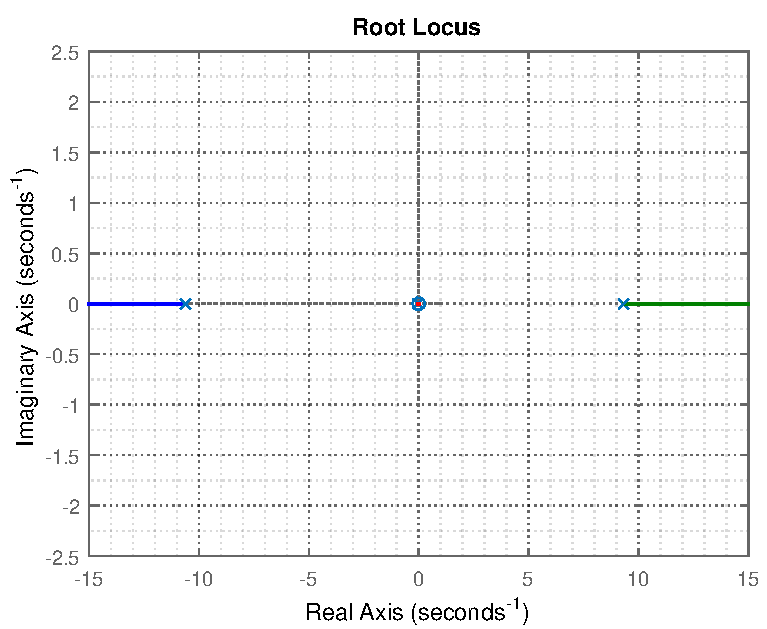
\includegraphics[scale=.56]{figures/rlocusCubli}
 			\centering
 			\captionsetup{justification=centering}
 			\captionof{figure}{Root Locus of the system}
 			\label{rlocusCubli}
 		\end{figure}
 	\end{minipage}
 	\hspace{0.03\linewidth}
 	\begin{minipage}{0.45\linewidth}
 		\begin{figure}[H]\vspace{4mm}
 			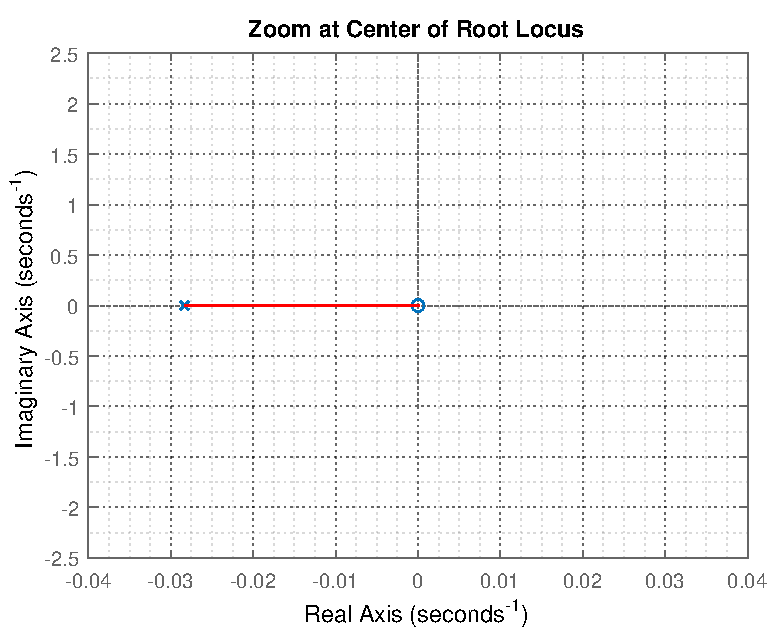
\includegraphics[scale=.56]{figures/rlocusCubliZoom}
 			\centering
 			\captionsetup{justification=centering}
 			\captionof{figure}{Zoom of \figref{rlocusCubli} from s=-0.04 to s=0.04}
 			\label{rlocusCubliZoom}
 		\end{figure}
 	\end{minipage}
\end{minipage}

\subsection{Nyquist Plot}
In any transfer function, the zeros of 1+L(s) (L(s) being the open loop function) become the poles of the closed loop system. That is why it is interesting to look at the Nyquist Stability Criterion, which can give information about this topic.

The number of zeros in the RHP of 1+L(s) (\si{Z_{RHP}}) is given by the number of poles of L(s) (\si{P_{RHP}}) and the number of clockwise encirclements of the Nyquist plot around -1 (\si{N}) (a counterclockwise circle has a negative sign in this equation).
%
\begin{flalign}
	\eq{Z_{RHP}}{N+P_{RHP}} 
	&\nonumber\\
	\label{ZNP}
\end{flalign}
%
For the system to be stable (\si{Z_{RHP}}) has to be zero, which means that there is no pole of the close loop function in the RHP.

In the case of this plant, the number of poles of L(s)=G(s) in the RHP is one and there are no encirclements of -1 in the Nyquist plot (\figref{nyquistCubli}). That results in one zero in the RHP. As this zero will be a pole in the closed loop, the system is confirmed as unstable.

\begin{figure}[H] 
	\centering 
	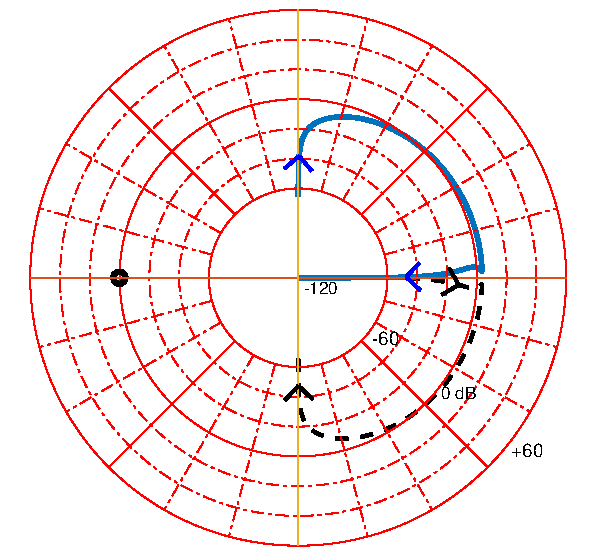
\includegraphics[scale=0.75]{figures/nyquistCubli}	
	\caption{Nyquist plot of the plant.}
	\label{nyquistCubli}
\end{figure}			        %-------- Stability Analysis
	
	%---------- Chapter 7 ---------------------------------------- Requirements
	\chapter{Design Specifications}\label{chap:specifications}


\section{Requirements}\label{requirements}
Based on the design considerations and limitations explained earlier in this report, a list of requirements shall be developed.
%
\begin{enumerate}
\item \textbf{The Cubli should be able to balance from an unstable equilibrium position and a null velocity.}
  \begin{itemize}
  \item[] Considering only naturally occurring perturbations, the Cubli needs to be able to regulate its position by itself, around the \si{0\ rad \cdot s^{-1}}, without falling directly.
  \end{itemize}

\item \textbf{The prototype should be able to balance around \si{0 \rad \cdot s^{-1}} regardless of the level of the baseplate, using internally mounted sensors.}  
  \begin{itemize}
  \item[] This ensures that the 2D design of the Cubli can keep its upright position independently from its base plate and therefore, can be more easily translated to a 3D model.
  \end{itemize}
%  
%\item \textbf{The Cubli should be balancing during X \si{s}.}\fxnote{A number should be determined for X.}
%  	\begin{itemize}
%  		\item[] The amount of time the system stands should be measured from the moment the controller starts acting on the plant, with initial conditions an unstable equilibrium position (aproximately \si{0\ rad \cdot s^{-1}}) with a null velocity of the wheel and the frame. The timer should be stopped as soon as the Cubli falls outside of the active region of the controller.
%  	\end{itemize}
%  	
%\item \textbf{The implemented controller should keep the Cubli within X \si{rad \cdot s^{-1}}.}\fxnote{A number has to be determined for Xand more arguments should be given.}
\end{enumerate}
%
From these established requirements, a controller allowing the Cubli to stabilize in an upright position is to be designed and implemented.

\section{Further Capabilities Analysis}\label{title}
Moreover, a further investigation on the behavior of the controlled system is to be done in order to determine the capabilities of the final prototype. This includes:
\begin{enumerate}
\item \textbf{Duration of the stable operation}
	\begin{itemize}
	\item[] How long can the Cubli be in equilibrium until the controller in not able to balance it.
	\end{itemize}

	\item \textbf{Maximum recovery angle}
	\begin{itemize}
		\item[] Once the Cubli is balance, its position is forced to change to different angles and the capability of tit to go back to the equilibrium position is checked. 
	\end{itemize}
	
	\item \textbf{Maximum catching angle with no initial velocity of the wheel}
	\begin{itemize}
		\item[] The maximum starting angle the system can have and still be able to balance is to be tested.\\
		However, there exists a limitation which is given by the maximum current that the motor can provide which conditions the maximum catching angle. As can be seen in \figref{limitationTorque}, if the initial angle is different from 0 rad both the mass of the frame ans the mass of the wheel exert an initial torque to the system. This must be overcame by the motor to avoid the Cubli to fall.
		%
		\begin{figure}[H] 
			\centering
			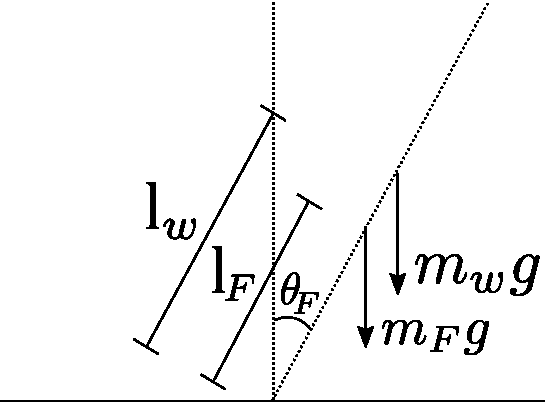
\includegraphics[scale=0.65]{figures/limitationTorque}
			\caption{Force acting on the system that create an initial torque}
			\label{limitationTorque}
		\end{figure}
		
		The minimum torque that the motor must apply is give by \eqref{minTorque}.
		%
		\begin{flalign}
		\eq{T} { (m_F \cdot l_F + m_w \cdot l_w) \cdot g \cdot sin(\theta_F)} \unit{N\cdot m}
		\label{minTorque}
		\end{flalign}
		
		Since the torque is restricted by the characteristics of the motor and the control board, the maximum initial angle is derived in \eqref{maxAngle}.
		%
		\begin{flalign}
		\eq{\theta_F} { asin\left(\frac{T}{(m_F \cdot l_F + m_w \cdot l_w) \cdot g}\right)} \unit{N\cdot m}
		\label{maxAngle}
		\end{flalign}
		%
		Substituding the values of the maximum torque (see section \ref{sec:Motor}) and the parameters of the Cubli (see section \ref{sec:Param}) the maximum starting angle is \si{0,2024\ rad}.

	\end{itemize}
	
\end{enumerate}
	
	%%% Part 2 %%%
	\part{Design \& Implementation}
	%---------- Chapter 8 ---------------------------------------- Classical Control Design
	\chapter{Classical Controller Design}\label{chap:controllerDesign}
The controller design is a very wide field that goes from classic linear PID controllers to more advanced techniques using numerical optimization.

In this chapter, a controller is designed using classical techniques. It is further analyzed to verify that the results fulfilled the requirements.

	\section{Root Locus Design}\label{rLocus}
The Root Locus of a transfer function is a plot of all the possible positions of the closed loop poles when applying a proportional gain K. The number of poles will be the same as the ones in the open loop case and each of them will have an associated branch that shows how it moves along with K. The plot has the following main characteristics:
%
\begin{itemize}
	\item[-] The plot is symmetric with respect to the real axis.
	\item[-] The number of branches, defined as n, is equal to the number of poles in the open loop function.
	\item[-] There are m branches that end in the zeros of the open loop function, m being the number of zeros.
	\item[-] There are n-m branches going to infinity.
	\item[-] The position of the poles changes the behavior of the system as seen in \figref{rLocusStability}
\end{itemize}
%
\begin{figure}[H] 
	\centering 
	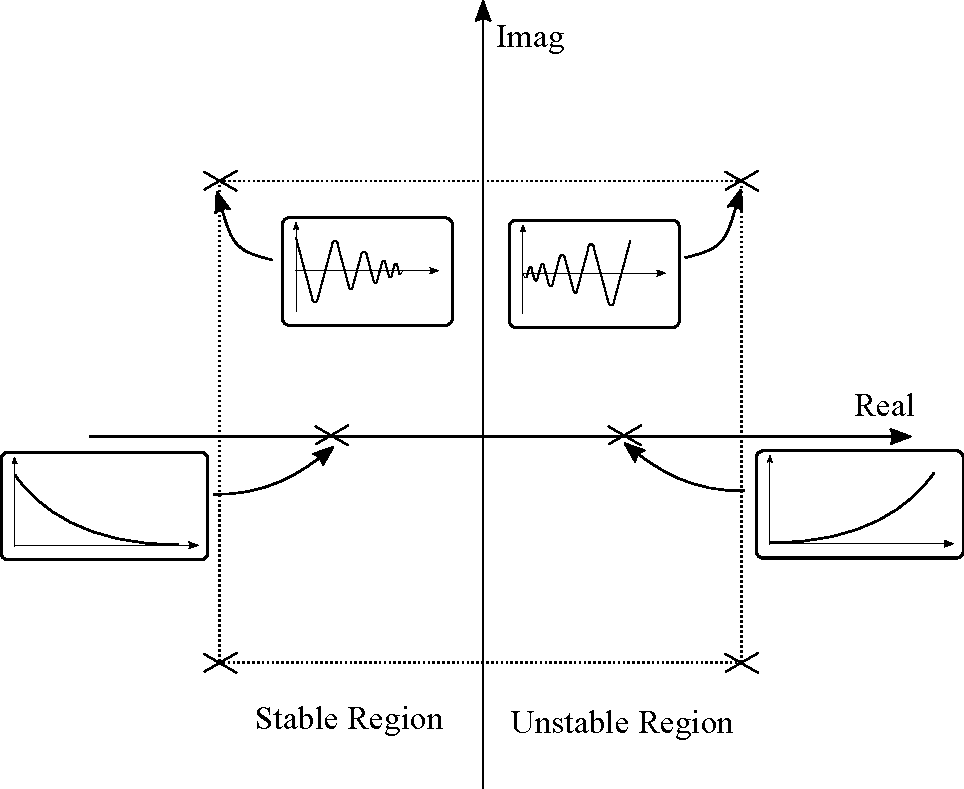
\includegraphics[scale=0.55]{figures/rLocusStability}	
	\caption{Response of a system depending on the position of its poles.}
	\label{rLocusStability}
\end{figure}
%
Root Locus design of controllers is based on the fact that the closed loop poles of a system will depend on the poles, zeros and gain of the open loop function. Knowing how the plot changes with the addition of poles and zeros, the branches can be modified to place the poles of the closed loop function where needed.
			      %-------- Root Locus Theory
	\section{Closed Loop Response}\label{closedLoop}
A first approximation to the behavior of the system in closed loop can be done through a proportional controller.

When a gain of 10 is put in the controller, the response of the simulation and the one from the real setup are the ones shown in \figref{closedLoopResponse}

\begin{figure}[H] 
	\centering 
	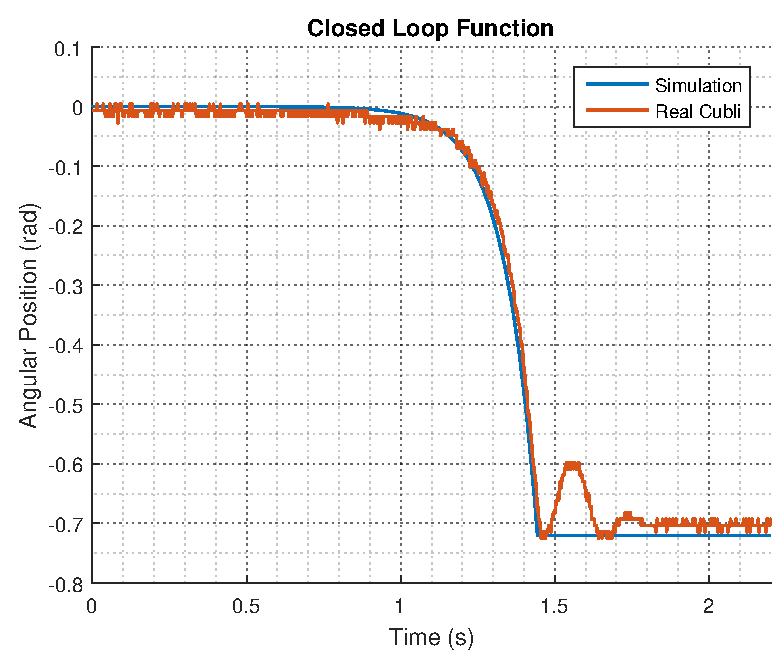
\includegraphics[scale=0.6]{figures/closedLoopResponse}	
	\caption{Behavior of the closed loop function with a proportional controller and both in simulation and reality}
	\label{closedLoopResponse}
\end{figure}

It is clear that the closed loop function has an unstable response when a reference of 0 rad is required.
			            %-------- Closed Loop response
	\section{Design of the Controller}\label{designController}
The design of the controller is based on the Root Locus plot, where the final location of the poles in closed loop can be seen. Their position will depend on the different poles, zeros and gain of the controller and that is used to move them to a stable and better location.

The root locus of the system can be seen in \figref{rlocusCubli2}.

\begin{figure}[H]
	\centering 
	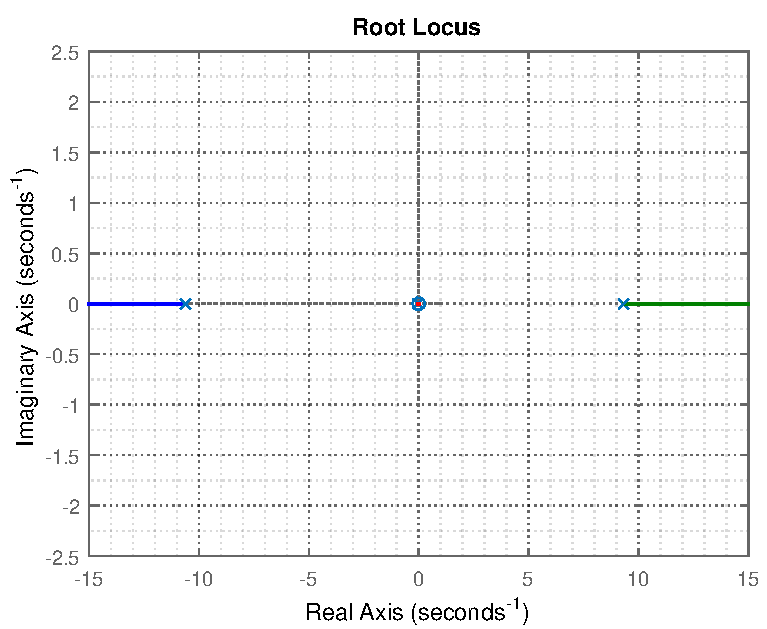
\includegraphics[scale=.56]{figures/rlocusCubli}
 	\captionof{figure}{Root Locus of the system}
 	\label{rlocusCubli2}
\end{figure}
%
As there exist one pole in the Right Half Plane (RHP), the controller must also have one there to create two branches which can be attracted to the Left Half Plane (LHP).

Then, two zeros must be placed in the LHP to make the branches enter in the stable region of the plot.

It is also important that the number of poles must be greater that the number of zeros for the controller to be feasible in reality. this means that two poles need to be placed somewhere so they don't affect the behavior of the final system. This can be achieve if they are placed in the LHP and far from the imaginary axis.

Finally, the gain must be adjusted to make the closed loop poles to be in a stable location. The resultant Root Locus can be seen in \figref{RLControllerZoom}.

\begin{figure}[H]
	\centering 
	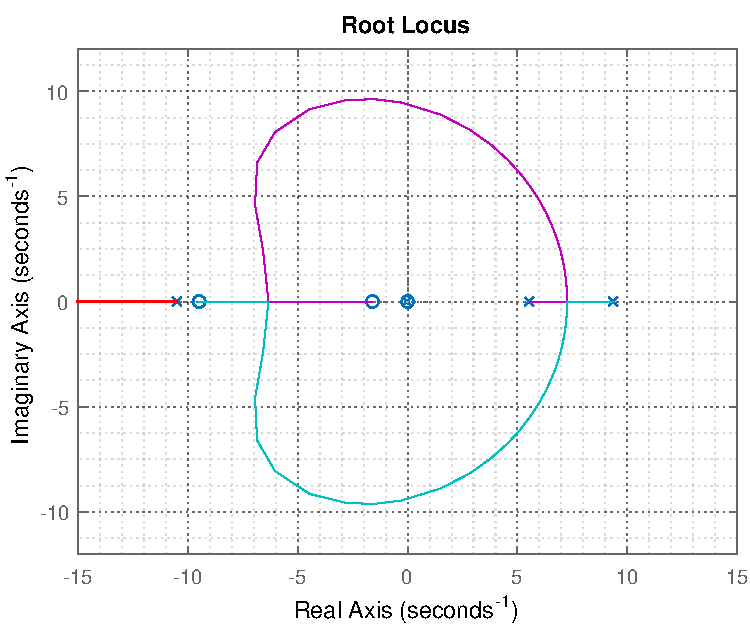
\includegraphics[scale=.56]{figures/RLControllerZoom}
	\captionof{figure}{Root Locus of the final system}
	\label{RLControllerZoom}
\end{figure}
%
The equation of final controller is then given by \eqref{ControllerLaplace}.

\begin{flalign}
	\eq{D(s)} {0,62737 \cdot \frac{(0,1054\ s + 1)\cdot (0,6254\ s + 1)}{(0,1805\ s - 1) \cdot (0,01\ s + 1) \cdot (0,005\ s + 1)}} & \nonumber\\
	\label{ControllerLaplace}
\end{flalign}
%
The stability of the controller given by \eqref{ControllerLaplace} can be then analyze using the Nyquist plot of the controller and the plant together, as seen in \figref{nyquistController}.

\begin{figure}[H] 
	\centering 
	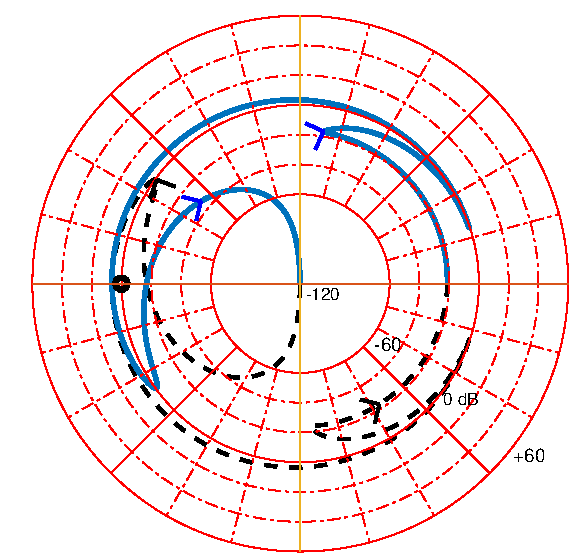
\includegraphics[scale=0.46]{figures/nyquistController}	
	\caption{Nyquist plot of the system with the controller}
	\label{nyquistController}
\end{figure}

Now the number of poles in the RHP is two and the number of encirclements around -1 is equals -2 (they are counterclockwise). This means that the system is stable, as the number of zeros in the RHP becomes 0.			      %-------- Design of the Controller
	\section{Implementation of the Controller}\label{impController}
The designed controller is shown to be working in the simulation environment. The next step is to actually implement it in reality.

Since the controller calculations are to be implemented on the Beaglebone Black board, which is a computer and cannot run continuously, the controller has to go through a discretization. This means that an approximation of it is made in the discrete domain.	  %-------- Implementation
	%\subsection{Discretization of the Controller}\label{ssec:discnController}
The discretization process of a controller consists in using the map from the continuous domain to the discrete domain (z-domain), with respect to the sampling time, \si{T}, of the feedback control system:
%
\begin{flalign} 
  &\si{s = j \omega \to z = e^{s T}}\label{exp:cont2Disc}&
\end{flalign}
%
Since, by definition, the discrete domain cannot represent the complete behavior of a system through time, approximations are used to estimate this behavior. Different methods are briefly described and compared hereafter in this subsection.

The most direct method is the Zero-Order Hold (ZOH) approximation. It mimics a Digital to Analog Converter's output behavior by holding a value of a certain amplitude during a time as long as the defined sampling time. Although, it matches reality correctly as long as the signal does not change too much between each sample, it does not fit as well at high frequencies. Thus, it translates into phase lag in the frequency domain and can cause trouble in closed-loop systems.\\
Another of the most commonly used aproximations is the bilinear transform (or Tustin's method) which is based on the trapezoidal integration principle. A reason to use this method instead of others is that it maps the entire LHP (stable area in the continuous domain) into the unit circle (stable area in the discrete domain)\cite{GFranklin}.\\
The bilinear approximation of \si{z} is defined as:
%
\begin{flalign} 
  &\si{z \approx \frac{1 + s \frac{T}{2}}{1 - s\frac{T}{2}}}\label{exp:bilinearTransform}&
\end{flalign}
%
The inverse transformation of \expr{exp:bilinearTransform} is given by:
%
\begin{flalign} 
  &\si{s \approx \frac{T}{2} \cdot \frac{1 - z^{-1}}{1 + z^{-1}}}\label{exp:inverseBilinearTransform}&
\end{flalign}
%
In general, the \expr{exp:inverseBilinearTransform} is used to replace \si{s} in the continuous-time transfer function of the designed controller. However, due to the non-linear mapping induced by the discretization, a pre-warp of the frequencies can be used before. This avoids effects of phase lag near the cross-over frequency and thus, also avoids unwanted reduction of gain and phase margins, see \cite{GGu,AVOppenheim}. 

Moreover, Matlab has an available function, \lstinline{c2d()}, designed to convert a continuous system's transfer function into the discrete domain by specifying the sampling time (here, \si{T = 0,01s}\fxnote{A justification fo this sampling time should be added at some point.}) and the desired method (\lstinline{'zoh'}, \lstinline{'tustin'} or \lstinline{'prewarp'}). When using the \lstinline{'prewarp'} option, a supplementary argument is needed, corresponding to the critical fequency, see \cite{Matlabc2d}.\\
Here, it is chosen to use \si{33,5\ rad \cdot s^{-1}} as the critical pre-warp frequency, as it corresponds to the point at which the phase lag is at its maximum on the open loop Bode plot of the continuous plant and controller, see \figref{fig:bodeOpenLoopContinuous}.
%
\begin{figure}[H]
  \centering
  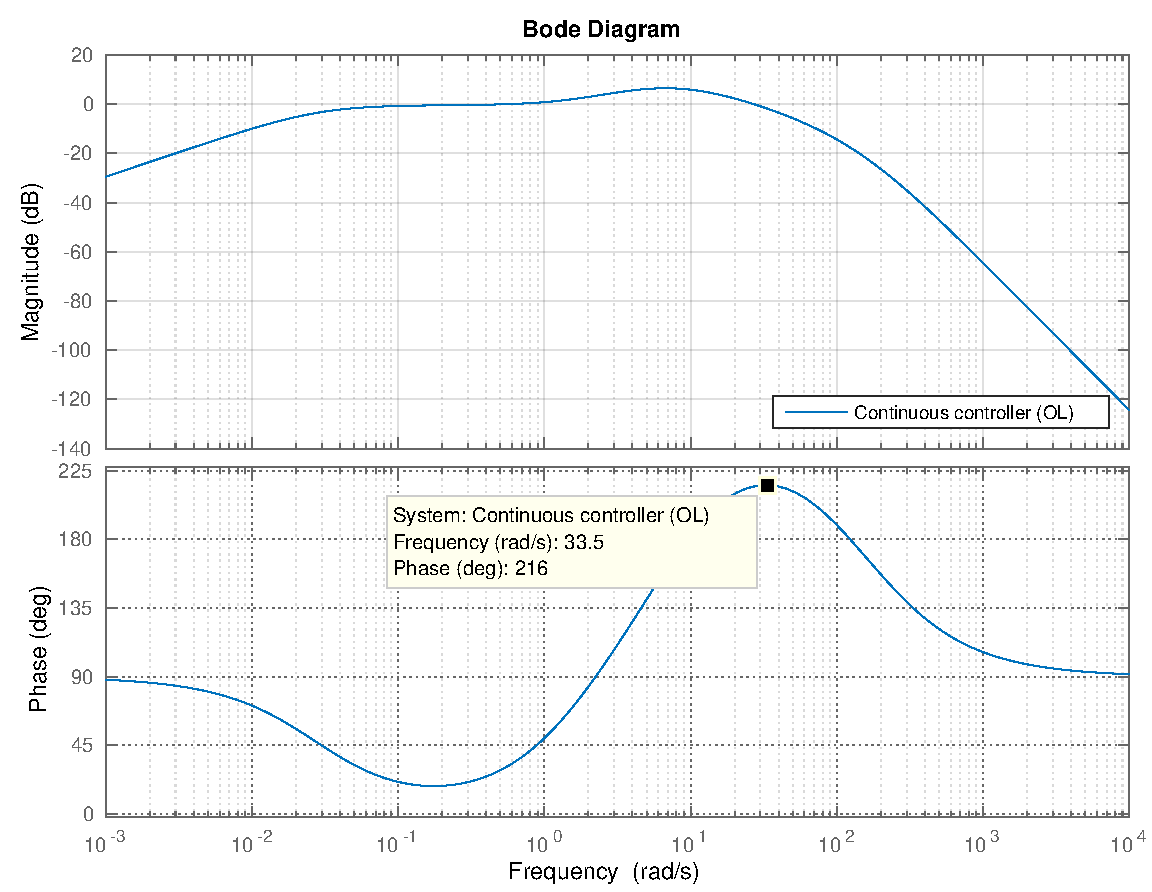
\includegraphics[scale=0.55]{figures/openLoopBadSISOController.pdf}
  \caption{Bode plot of the continuous open loop system}
  \label{fig:bodeOpenLoopContinuous}
\end{figure}
%
\Figref{fig:bodePrewarpVsNoPrewarpVsContinuousOpenLoop} shows Bode plots comparing open loops with the original continuous controller agaisnt the discretized controller's with ZOH, normal Tustin's method and pre-warping, while \figref{fig:bodePrewarpVsNoPrewarpVsContinuousClosedLoop}, shows the system's closed loop responses with these controllers.\\ 
%
\begin{figure}[H]
  \centering
  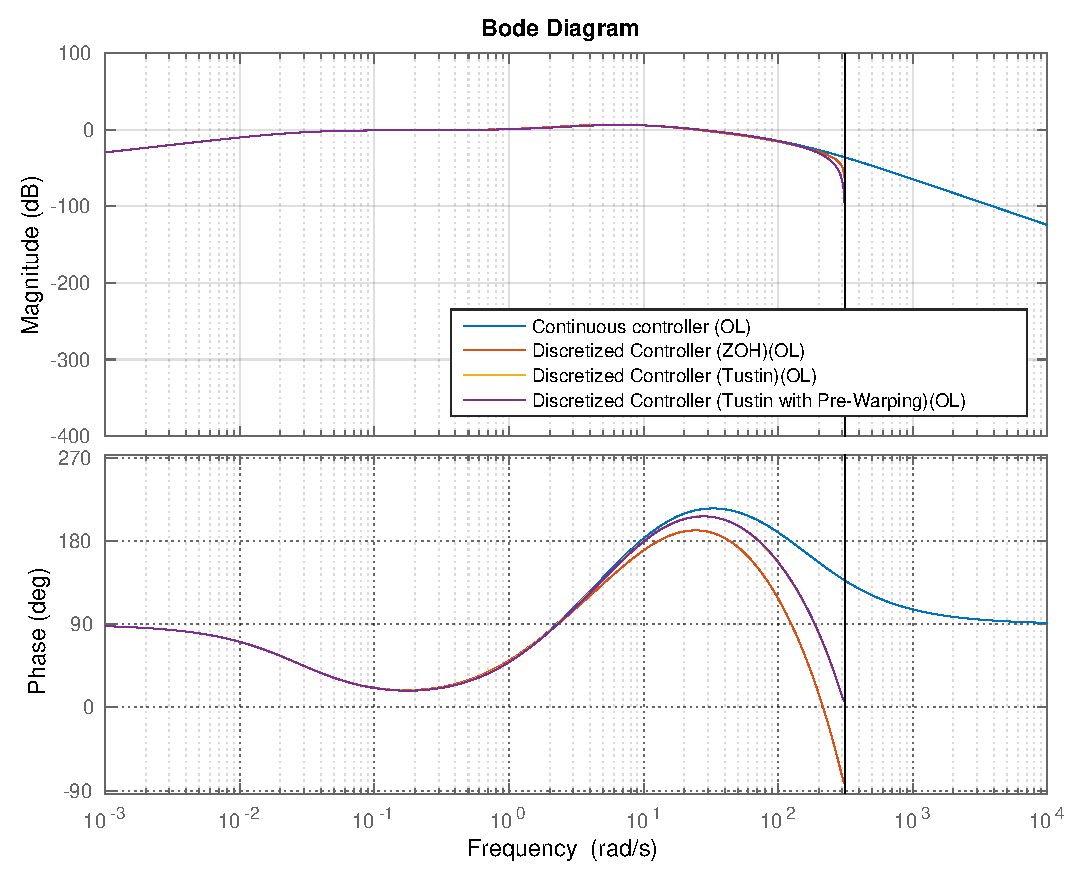
\includegraphics[scale=.6]{figures/zohVsPrewarpVsNoPrewarpVsContinuousBodeOpenLoop.pdf}
  \caption{Bode plot of the open loop system with the continuous controller (in blue), ZOH discretized controller (in red), Tustin discretized controller (in orange) and pre-warped Tustin discretized controller (in purple)}
  \label{fig:bodePrewarpVsNoPrewarpVsContinuousOpenLoop}
\end{figure}
%
From \figref{fig:bodePrewarpVsNoPrewarpVsContinuousOpenLoop}, it is possible to see that the phase of the ZOH discretized controller diverges from the continuous one's, no later than at \si{3\ rad \cdot s^{-1}}. On the other hand, Tustin discretized controllers match closely with the continuous one until approximately \si{10^{1}\ rad \cdot s^{-1}}. \\
The discrete systems here, are only plotted before the vertical line which represents the Nyquist frequency, i.e.~a half of the sampling frequency, chosen earlier in this section\fxnote{If the frequency choic is further explained, the corresponding section should be used as a reference here.}. More importantly, the two discrete versions of the controller, the orange one using a simple Tustin method and the purple one using also pre-warping, seem very similar both in frequency and phase.
%
\begin{figure}[H]
  \centering
  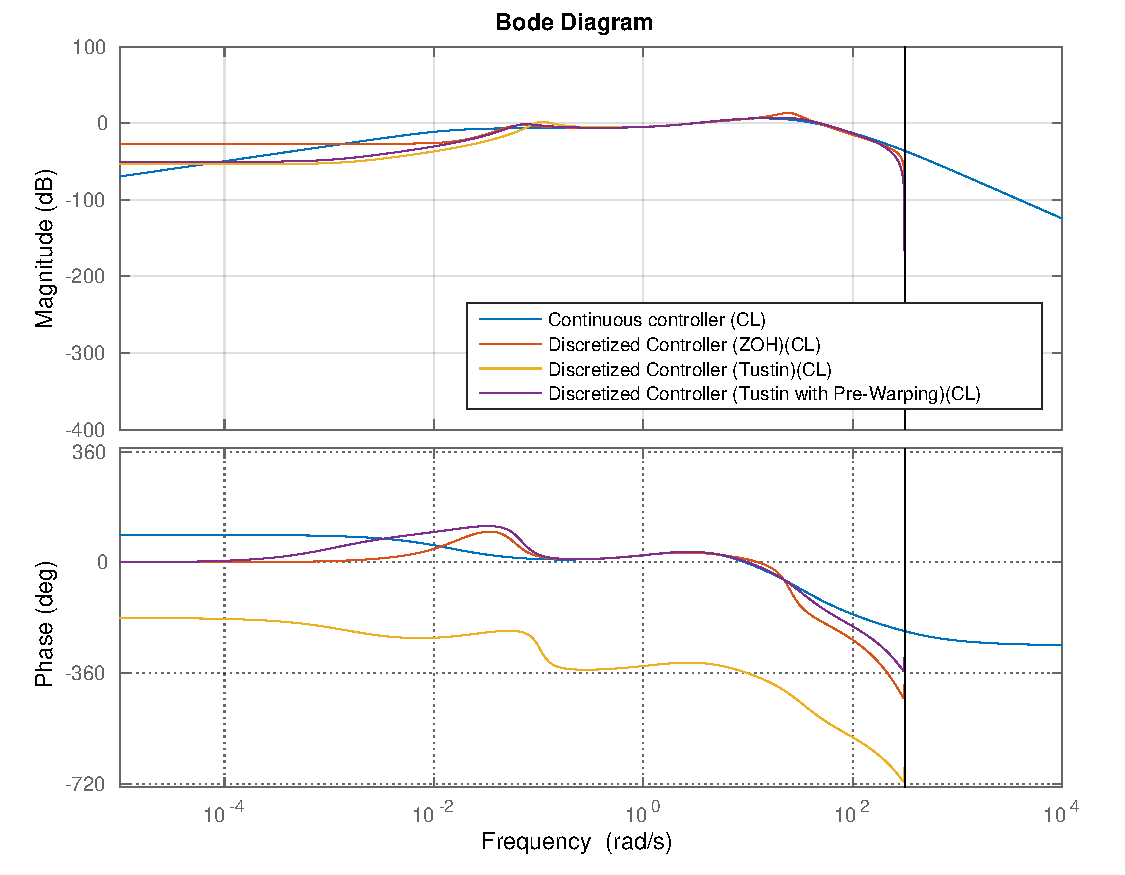
\includegraphics[scale=.6]{figures/zohVsPrewarpVsNoPrewarpVsContinuousBodeClosedLoop.pdf}
  \caption{Bode plot of the closed loop system with the continuous controller (in blue), ZOH discretized controller (in red), Tustin discretized controller (in orange) and pre-warped Tustin discretized controller (in purple)}
  \label{fig:bodePrewarpVsNoPrewarpVsContinuousClosedLoop}
\end{figure}
%
More than with the open loop Bode plot, a difference between controllers is visible by looking at the closed loop Bode plot, on \figref{fig:bodePrewarpVsNoPrewarpVsContinuousClosedLoop}. There, it is apparent that the phase of the pre-warped controller follows more closely the phase of the continuous version than with only Tustin approximation, which is desirable. On the contrary, the non-pre-warped discrete controller has a huge phase lag of at least \si{180^{\circ}} compared to the continuous closed-loop which reveals a substantial delay.\fxnote{Add more to justify pre-warp instead of zoh}

Thus, the pre-warped discretized controller is chosen for the actual implementation on the Cubli, in the code base, see \secref{sec:codeBase}, and its discrete transfer function is:
\begin{flalign}
  \eq{D(z)} {\frac{\tau_{m,w}(z)}{e_{\theta}(z)} = \frac{\num{-8,314} + \num{7,422} \cdot z^{-1} + \num{8,302} \cdot z^{-2} - \num{7,434} \cdot z^{-3}}{1 - \num{1,382} \cdot z^{-1} + \num{0,3415} \cdot z^{-2} + \num{0,001638} \cdot z^{-3}}} &%\unit{N \cdot m} 
  \label{eq:discControllerTf}
\end{flalign}
To implement a discrete controller in a code environment, the preferred form is the difference equation. This is why \eqref{eq:discControllerTf} is transformed into:
\begin{flalign}
  \eqOne{\tau_{m}[n]}{\num{-8,314} \cdot e_{\theta}[n]+ \num{7,422} \cdot e_{\theta}[n-1] + \num{8,3023} \cdot e_{\theta}[n-2] - \num{7,434} \cdot e_{\theta}[n-3] }
  \eqTwo{+ \num{1,382} \cdot \tau_{m}[n-1] - \num{0,3415} \cdot \tau_{m}[n-2] - \num{0,001638} \cdot \tau_{m}[n-3]}\unit{N \cdot m} 
  \label{eq:discControllerDiffEq}
\end{flalign}
%
\hspace{6mm} Where:\\
\begin{tabular}{ p{1cm} l l l}
& \si{\tau_{m}}         & is the wanted motor torque                                      &\unitWh{N \cdot m} \\
& \si{e_{\theta}}         & is the error between wanted and measured frame angle          &\unitWh{rad}\\
& \si{x[n-m]}             & is the m-th previous state of a signal x, m = 0,1,2,3         &\unitWh{\cdot}\\
\end{tabular}

In this subsection, the designed controller has been discretized. The next subsection goes into further analysis of the new feedback control system before and after the actual implementation on the real system.   %-------- Discretization
	\section{Controller Analysis}\label{ssec:ControllerVerification}
A further analysis can be done to the controller, both continuous and discrete, and also to the real response of the system once it is implemented.

The first step is to simulate both the continuous and discrete controller with the model of the system and analyse the behavior of the whole closed loop system.

This is done not only to see the behavior of the designed controller but also to verify that the discretized controller matches the original continuous one. 

With a constant reference of 0 rad and a disturbance in the form of a torque applied to the frame of \si{0,55 Nm}, the responses are the ones shown in \figref{discreteVsContinuousOutputController} and \figref{discreteVsContinuousSimulation}.
%
\begin{minipage}{0.45\linewidth}
	\begin{figure}[H]
      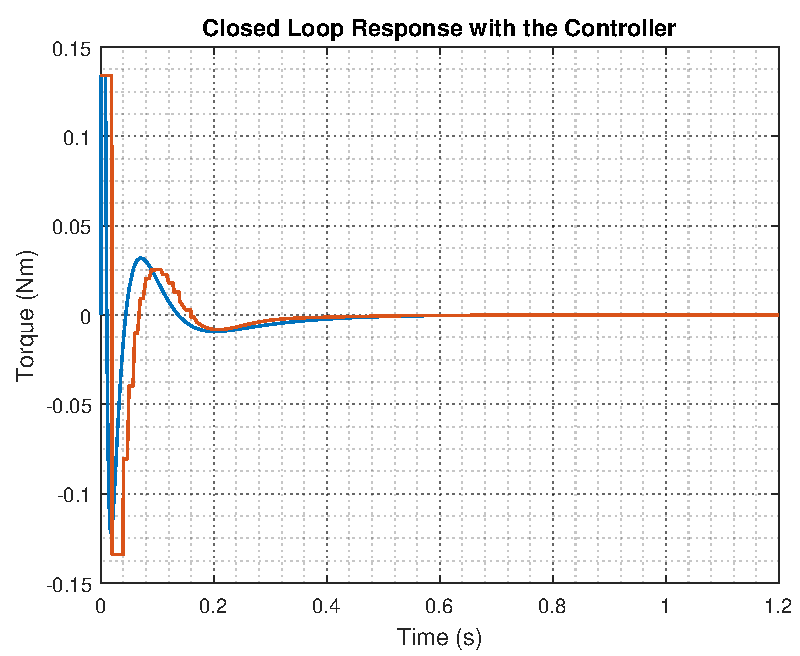
\includegraphics[scale=.53]{figures/torqueComp}
      \captionsetup{justification=centering}
      \captionof{figure}{Controller's output (torque) response in the control loop with the continuous (blue) and discrete (red) controllers}
      \label{discreteVsContinuousOutputController}
    \end{figure}\vspace{-5mm}
\end{minipage}
\hspace{0.03\linewidth}
\begin{minipage}{0.45\linewidth}
    \begin{figure}[H]\vspace{-4mm}
      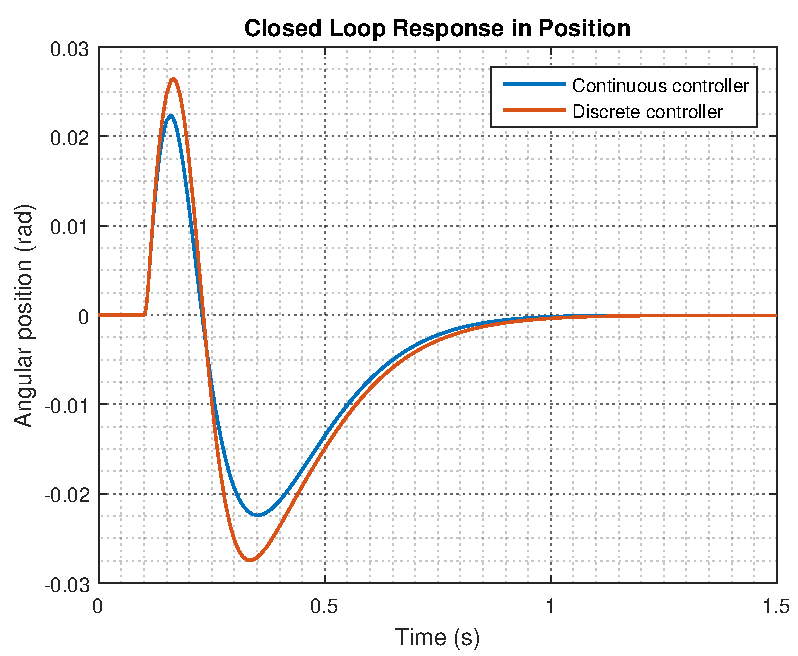
\includegraphics[scale=.53]{figures/positionComp}
      \captionsetup{justification=centering}
      \captionof{figure}{Closed loop response of the continuous (blue) and discrete (red) controllers}
      \label{discreteVsContinuousSimulation}
    \end{figure}\vspace{-5mm}
\end{minipage}

Both controllers seem to have a good behavior and both reach the desired final position in simulation. However after testing the controller on the cubli, it was discovered that it is important to also look at the velocity of the wheel. It has been assumed to be 0 in the equilibrium position, and that is not the case.\fxnote{add some eplanation with test result on the problem}
%
\begin{figure}[H]\vspace{-4mm}
	\centering
	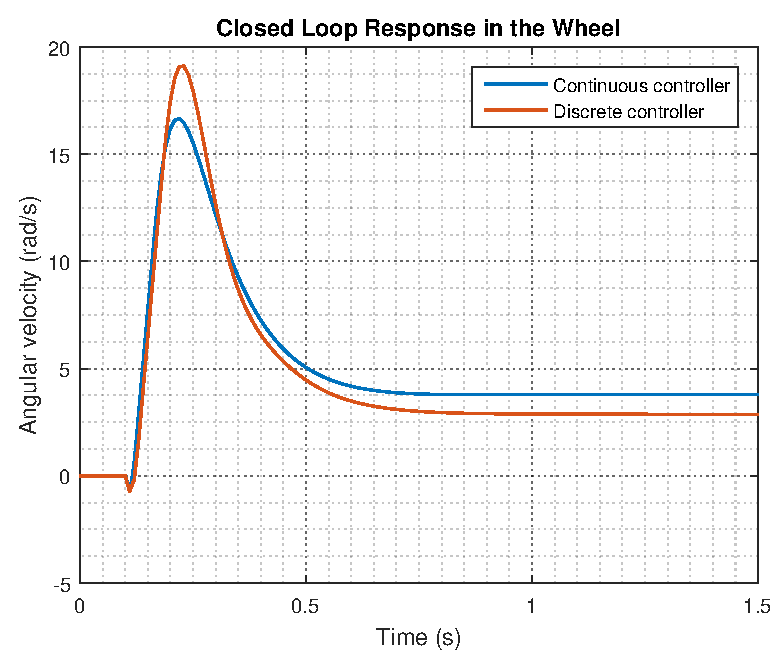
\includegraphics[scale=.53]{figures/wheelComp}
	\captionof{figure}{Angular velocity of the wheel}
   \label{fig:discreteVsContinuousWheel}
\end{figure}\vspace{-5mm}

In both cases the velocity is different from 0 in steady state. It should not be any problem since a constant velocity does not produce any torque 
to the system. However there is friction in the wheel, which will make it to slow down, producing an acceleration on the system. This will make the Cubli to slightly move from equilibrium position and the controller will try to apply some torque to the system to balance it. The problem arises if the motor was already very closed to its maximum speed and it will not be able to accelerate more and produce the torque needed, making the frame fall over.

The conclusion is that the controller is not able to ensure zero velocity in equilibrium with only a feedback in the position of the frame. This means that another kind of controller, which also takes care of the velocity of the wheel, may result in a better behavior.

One way could be using a cascade controller to control both the velocity of the wheel and the position of the frame. In \figref{cascadeControl} it can be seen the block diagram for a cascade control, with the particularity of a feedback from the position of frame to the velocity of the wheel.

\begin{figure}[H]
	  \begin{tikzpicture}[ auto,
thick,                         %<--setting line style
node distance=2cm,             %<--setting default node distance
scale=1.0,                     %<--|these two scale the whole thing
every node/.style={scale=1.0}, %<  |(always change both)
>=triangle 45 ]                %<--sets the arrowtype
  ]
  
  %-- Blocks creation --%
  \draw
	node[shape=coordinate][](ref) at (0,0){\si{\theta_F}}			% start of reference
 
	node(sum1) at (2,0) [sum] {$\sum$}
 
	node(D2) at (4,0) [block] {$D2$}
	
	node(sum2) at (6,0) [sum] {$\sum$}
	
	node(D1) at (8,0) [block] {$D1$}
	
	node(G1) at (10,0) [block] {$G1$}
	
	node[shape=coordinate][](velFeed) at (11,0){omega\_f}
	
	node(G2) at (12,0) [block] {$G2$}
	
	node[shape=coordinate][](feed) at (13,0){feed}
	
	node[shape=coordinate][](angleFeed) at (14,0){theta\_f}
	
	node[shape=coordinate][](out) at (15,0){theta\_f}
	
	% - feedback nodes
	
	node[shape=coordinate][](feed1) at (9,-1.5){feed1}
	
	node[shape=coordinate][](feed2) at (9,-2){feed2}
	
	node[shape=coordinate][](feed3) at (12,-1){feed3}
	
  ;
  
  \draw[->](ref) -- node {\si{\theta_F}} (sum1);
  
  \draw[->](sum1) -- node {} (D2);
  
  \draw[->](D2) -- node {} (sum2);
  
  \draw[->](sum2) -- node {} (D1);
  
  \draw[->](D1) -- node {} (G1);
  
  \draw[->](G1) -- node {\si{\dot{\theta}_F}} (G2);
  
  \draw[->](G2) -- node {\si{\theta_F}} (out);
  
  % - drawing feedback lines
  
  \draw[-](velFeed) |- node {} (feed1);
  
  \draw[-](angleFeed) |- node {} (feed2);
  
  \draw[-](feed1) -| node {} (sum2);
   
  \draw[-](feed2) -| node {} (sum1);
  
  \draw[dashed](feed) |- node {} (feed3);
  
  \draw[dashed, ->](feed3) -| node {} (G1);
  
  % - adding + and - at the sum nodes
    \draw
  node at (sum1) [right = -6.6mm, below = .6mm] {$+$}
  node at (sum1) [right = -3mm, below = 3.9mm]  {$-$} 
  
  node at (sum2) [right = -6.6mm, below = .6mm] {$+$}
  node at (sum2) [right = -3mm, below = 3.9mm]  {$-$} 
  ;
 
  
  \end{tikzpicture}
	\centering
	\caption{Block diagram for a cascade control (the dotted line corresponds to a feedback in the Cubli system that is not present in the normal cascade control)}
	\label{cascadeControl}
\end{figure}

The problem of this solution in the case of the Cubli is that both variables to control are coupled together, which means that it is not possible to split the plant in a way that there is no feedback between them.\cite{LRusso}

Another way is to use an state space approach, which can handle this singularity, since now the system will have two outputs to control. This controller solution is further detailed in \chapref{chap:stateSpaceController}.
     %-------- Verification
	
	%---------- Chapter 9 ---------------------------------------- State Space Controller
	\chapter{State-Space Controller}\label{chap:stateSpaceController}
State-space representation describes a system with a set of first-order differential equations. This can be done through the use of state variables, which describe internal states of the system. This representation gives a very convenient way of analyzing systems that have several inputs and outputs.

In this chapter the state-space description of the system is derived and a controller capable of maintain it in equilibrium position is designed.


	\section{State Space Representation of the System}\label{sec:SSDescription}
The first step to give a representation of the system in state space is to choose the input, output and state variables. In this case the state variables are chosen to be the position of the frame and the velocities of frame and wheel (\si{\theta_F,\ \dot{\theta}_F,\ \dot{\theta}_w}). The input is the torque from the motor (\si{\tau_m}) and the chosen outputs are  the ones to control, (\si{\theta_F,\ \dot{\theta}_w}).
%
\begin{minipage}{0.32\linewidth}
	\begin{flalign}
		\vec{x} = 
		\begin{bmatrix}
			\theta_F \\
			\dot{\theta}_F \\ 
			\dot{\theta}_w \\
		\end{bmatrix}	\nonumber
		\label{xVector}
	\end{flalign}  
\end{minipage}\hfill
%\hspace{0.03\linewidth}
\begin{minipage}{0.32\linewidth}
	\begin{flalign}
		\vec{y} = 
		\begin{bmatrix}
			\theta_F \\
			\dot{\theta}_w \\
		\end{bmatrix}	\nonumber
		\label{yVector}
	\end{flalign}
\end{minipage}\hfill
%\hspace{0.03\linewidth}
\begin{minipage}{0.32\linewidth}
	\begin{flalign}
		\vec{u}= 
		\begin{bmatrix}
			\tau_m\\
		\end{bmatrix}
		\label{uVector}
	\end{flalign}
\end{minipage}\hfill

The relationship between them is  given in the form of first-order differential equations:
\begin{flalign}
	\eq{\vec{\dot{x}}}{f(\vec{x},\vec{u})}
	\label{xDotDiffEq} 
\end{flalign}
\begin{flalign}
	\eq{\vec{y}}{g(\vec{x},\vec{u})} 
	\label{yDiffEq} 
\end{flalign}
%
In this case f and g can be derived from \eqref{finalWheel} and \eqref{finalFrame} and they are non-linear functions since there exist a sinusoidal term in both.

However, it has been shown in \secref{sec:linearization} that a linear approximation near the equilibrium point is possible. Then, the system can be described in the form of linear state space equations as seen in \eqref{xDotLinear} and \eqref{yLinear}.
%
\begin{flalign}
	\eq{\vec{\dot{x}}(t)}{\vec{A} \cdot \vec{x}(t) + \vec{B} \cdot \vec{u}(t)}
	\label{xDotLinear} 
\end{flalign}
\begin{flalign}
	\eq{\vec{y}(t)}{\vec{C} \cdot \vec{x}(t) + \vec{D} \cdot \vec{u}(t)}
	\label{yLinear} 
\end{flalign}
%
\hspace{6mm} Where:\\
\begin{tabular}{ p{1cm} l l l}
	& \si{\vec{A}=\frac{\partial}{\partial \vec{x}} \ f(\vec{x_o},\vec{u_o})}			& is the \si{3x3}  state matrix     \\                       
	& \si{\vec{B}=\frac{\partial}{\partial \vec{u}} \ f(\vec{x_o},\vec{u_o})}			& is the \si{3x1}  input matrix       \\ 
	& \si{\vec{C}=\frac{\partial}{\partial \vec{x}} \ g(\vec{x_o},\vec{u_o})}			& is the \si{2x3}  output matrix      \\ 
	& \si{\vec{D}=\frac{\partial}{\partial \vec{u}} \ g(\vec{x_o},\vec{u_o})}			& is the \si{2x1}  feedforward matrix \\ 
\end{tabular} 
\\
The state space description can be seen also in the form of a block diagram like the one from \figref{SSBlocks}.
%
\begin{figure}[H]
	\begin{tikzpicture}[ auto,
                       thick,                         %<--setting line style
                       node distance=1.5cm,             %<--setting default node distance
                       scale=1,                     %<--|these two scale the whole thing
                       every node/.style={scale=1}, %<  |(always change both)
                       >=triangle 45 ]                %<--sets the arrowtype
    
    \draw%-----------------------------------------------------------------------------------------
    	%Drawing Input/Output:
    	node[shape=coordinate][](input1) at (0,0){}
    	node[shape=coordinate][](output1) at (9.5,0){}
     	%Drawing the Equation Blocks:   	
      	node(A) at (4.5,-1.5) [block] {A} 
     	node(B) at (1.5,0) [block] {B}
     	node(C) at (6.5,0) [block] {C}
      	node(D) at (4.5,1.5) [block] {D}  
	    node(int) at (4.5,0) [block] {\si{\int}}  
    	%Drawing the Sumation Blocks:	    	 	
    	node(sum1) [sum, right of = B] {\si{\sum}}
    	node(sum2) [sum, right of = C] {\si{\sum}}
    	%Drawing the Feedback/Feedforward Nodes:    	
    	node[shape=coordinate][](FeedforwardNode) at (0.75,0){}
    	node[shape=coordinate][](FeedbackNode) at (5.5,0){}  	
    	     
    ;%---------------------------------------------------------------------------------------------
   
    %Joining the Blocks
  	\draw[->](input1) -- node {u}(B);
  	\draw[->](B) -- node {}(sum1);
  	\draw[->](sum1) -- node {\si{\dot x}}(int);  	
  	\draw[->](int) -- node {x}(C);
  	\draw[->](C) -- node {}(sum2);  	
  	\draw[->](sum2) -- node {y}(output1);
  	
  	\draw[->](FeedforwardNode) |- node{} (D);
  	\draw[->](D) -| node{} (sum2);

  	\draw[-] (FeedbackNode) |- (A);
  	\draw[->] (A)   -| (sum1);

    %Drawing node(s) with \textbullet
    \draw%--------------------------------------------------------------
      node at (input1)  [shift={(-0.08, -0.02 )}] {\large \textbullet}
    	% node at (output1) [shift={( 0.008, -0.02 )}] {\textbullet}
    ;%------------------------------------------------------------------
  \end{tikzpicture}
	\centering
	\caption{Block diagram of the state space representation}
\end{figure} \label{SSBlocks}
%
This matrices can be obtained from the linearized equations of the system from \ref{sec:linearization}, given the final system description as \eqref{xDotSS} and \eqref{ySS}.

\begin{flalign}  \label{xDotSS}
	\si{\vec{\dot{x}}(t)} &= 
	\begin{bmatrix}
		\si{0} & \si{1} & \si{0} \\
		\si{\frac{(m_F \cdot l_F + m_w \cdot l_w) \cdot g}{J_F + m_w \cdot {l_w}^2}} & \si{-\frac{B_F}{J_F + m_w \cdot {l_w}^2}} & \si{\frac{B_w}{J_F + m_w \cdot {l_w}^2}} \\
		\si{- \frac{(m_F \cdot l_F + m_w \cdot l_w) \cdot g}{J_F+m_w \cdot {l_w}^{2}}} & \si{\frac{B_F}{J_F+m_w \cdot {l_w}^{2}}} & \si{\frac{(J_w+J_F+{l_w}^{2} \cdot m_w) \cdot B_w}{J_w \cdot (J_F+m_w \cdot  {l_w}^2)}} \\
	\end{bmatrix}
	\si{\cdot \vec{x}(t) +}
	\begin{bmatrix}
		\si{0} \\
		\si{- \frac{1}{J_F + m_w \cdot {l_w}^2}} \\
		\si{\frac{J_w+J_F+m_w \cdot {l_w}^{2}}{J_w \cdot (J_F+m_w \cdot {l_w}^{2})}} \\
	\end{bmatrix}
	\si{\cdot \vec{u}(t)}&
\end{flalign}
\begin{flalign} \label{ySS}
	\si{\vec{y}(t)} &=
	\begin{bmatrix}
		\si{1} & \si{0} & \si{0} \\
		\si{0} & \si{0} & \si{1} \\
	\end{bmatrix}
	\cdot \vec{x}(t) +
	\begin{bmatrix}
		\si{0} \\
		\si{0} \\
	\end{bmatrix}
	\si{\cdot \vec{u}(t)}
\end{flalign}
%
Substituting the values for the parameter in \eqref{xDotSS} and \eqref{ySS} gives the final description for the system.
%

\begin{equation}  \label{xDotSSNum}
	\dot{\vec{x}}(t)  = 
	\begin{bmatrix}
		0 & 1 & 0 \\
		98,2208 & -1,1458 & 0,0025 \\
		-98,2208 & 1,1458 & -0,0309 \\
	\end{bmatrix}
	\cdot \vec{x}(t) +
	\begin{bmatrix}
		0 \\
		- 148,8077 \\
		1812,7013 \\
	\end{bmatrix}
	\cdot \vec{u}(t) 
\end{equation}
\begin{equation} \label{ySSNum}
	\vec{y}(t) = 
	\begin{bmatrix}
		1 & 0 & 0 \\
		0 & 0 & 1 \\
	\end{bmatrix}
	\cdot \vec{x}(t) 
\end{equation}	%-------- Description in State Space
	\section{System Analysis in State-Space}\label{sec:SSAnalysis}
The stability of the system can be derived from matrix A. The denominator of the transfer function of the system is equal to the characteristic polynomial of A, which means that its eigenvalues are the poles of the system. The eigenvalues of A are, as expected, \si{-10.5014,\ 9.3531\ and\ -0.0283}.

Once the system is confirmed as unstable, its controllability in state-space must be determine. It refers of the ability to go from one state to another in a finite amount of time by means of admissible inputs. To do that, the controllability matrix must be analyzed.
%
\begin{equation}  \label{controlability}
	controlability\ matrix = 
	\begin{bmatrix}
		A & AB & A^2B \\
	\end{bmatrix}
\end{equation}
%
The control matrix in this case is full row rank which means that the system is controllable.

Another important characteristic for the design of controllers is the observability, which refers to the capability of inferring the internal states knowing the outputs of the system. In this case there exists a matrix which includes only C and A, which meas that the observability is not related with the inputs of the system. 
%
\begin{equation}  \label{observability}
	observability\ matrix = 
	\begin{bmatrix}
		C \\
		CA \\
		CA^2 \\
	\end{bmatrix}
\end{equation}
%
This matrix has also full row rank so the states can be observed.	%-------- Analysis in State Space
	\section{Design of the Controller in State Space}\label{sec:SSController}
The aim of the controller is to maintain the system in equilibrium position, which means that the reference for each state is always zero. 

With this assumption a new state matrix can be created such that its poles are placed in the LHP and then the system becomes stable.This is done by adding a state feedback and a \si{3x1} gain matrix to the whole system, as seen in \figref{SSBlocksFeedback}.
%
\begin{figure}[H]
	\begin{tikzpicture}[ auto,
					thick,                         %<--setting line style
					node distance=1.5cm,             %<--setting default node distance
					scale=1,                     %<--|these two scale the whole thing
					every node/.style={scale=1}, %<  |(always change both)
					>=triangle 45 ]                %<--sets the arrowtype

	\draw%-----------------------------------------------------------------------------------------
	%Drawing Input/Output:
	node[shape=coordinate][](input1) at (0,0){}
	node[shape=coordinate][](output1) at (8,0){}
	%Drawing the Equation Blocks:   	
	node(A) at (4,-1.5) [block] {A} 
	node(B) at (1.5,0) [block] {B}
	node(C) at (6.5,0) [block] {C}
	node(int) at (4.5,0) [block] {\si{\int}} 
	node(K) at (3,-2.5) [block] {-K}	
	%Drawing the Sumation Blocks:	    	 	
	node(sum1) [sum, right of = B] {\si{\sum}}
	%Drawing the Feedback/Feedforward Nodes:    	
	node[shape=coordinate][](FeedbackNode) at (5.2,0){}  	
	node[shape=coordinate][](FeedbackNode2) at (5.6,0){} 
	
	;%---------------------------------------------------------------------------------------------

	%Joining the Blocks
	\draw[->](input1) -- node {u}(B);
	\draw[->](B) -- node {}(sum1);
	\draw[->](sum1) -- node {\si{\dot x}}(int);  	
	\draw[->](int) -- node {x}(C);
	\draw[-](C) -- node {y}(output1);

	\draw[->] (FeedbackNode) |- (A);
	\draw[->] (A)   -| (sum1);
	
	\draw[->] (FeedbackNode2) |- (K);
	\draw[-] (K)   -| (input1);

	%Drawing node(s) with \textbullet
	\draw%--------------------------------------------------------------
%	node at (input1)  [shift={(-0.08, -0.02 )}] {\large \textbullet}
	node at (output1) [shift={( 0.008, -0.04 )}] {\textbullet}
	;%------------------------------------------------------------------

\end{tikzpicture}
	\centering
	\caption{Block diagram with the state feedback}
\end{figure} \label{SSBlocksFeedback}
%
This new configuration gives a new equation for \si{\vec{\dot{x}}}:
%
\begin{flalign}
	\eq{\vec{\dot{x}}(\vec{t})}{(\vec{A}-\vec{B}\vec{K}) \cdot \vec{x}(\vec{t})}
	\label{xDotK} 
\end{flalign}
%
The objective is to find K such that the eigenvalues of \si{\vec{A}-\vec{B}\vec{K}} are placed at the LHP. This gain matrix can be found using the Matlab command \lstinline{place(A,B,P)}, where P is a vector containing the desired position of the new poles.

To choose the position of these poles two simulations are made for different values. In the first one the Cubli starts from equilibrium and a disturbance torque is applied while in the second one it starts from an initial angle different from \si{0\ rad} and with an initial acceleration.

\begin{minipage}{\linewidth}
	\begin{minipage}{0.45\linewidth}
		\begin{figure}[H]
			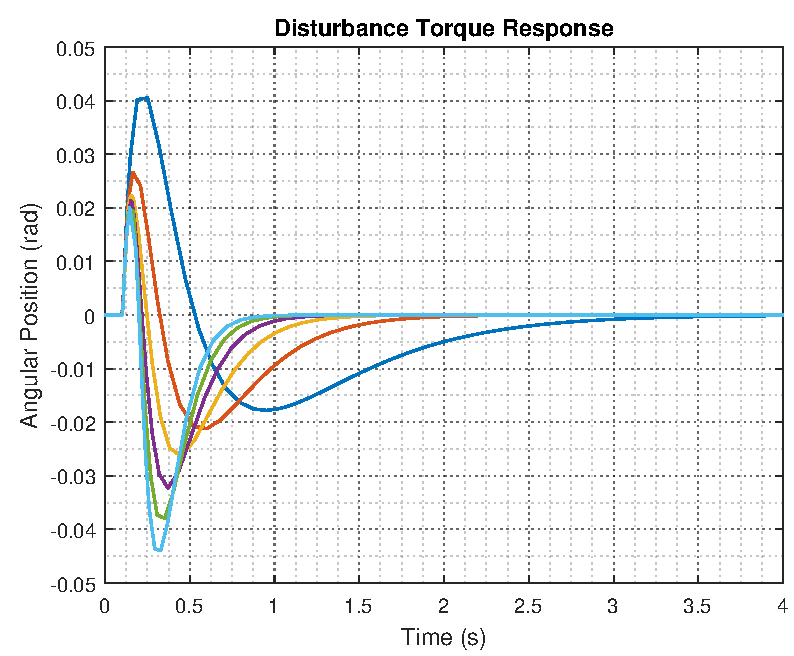
\includegraphics[scale=.55]{figures/disturbanceStateSpace}
			\centering
			\captionsetup{justification=centering}
			\captionof{figure}{Response of the system to a disturbance with different locations of poles}
			\label{disturbanceStateSpace}
		\end{figure}
	\end{minipage}
	\hspace{0.03\linewidth}
	\begin{minipage}{0.45\linewidth}
		\begin{figure}[H]\vspace{0mm}
			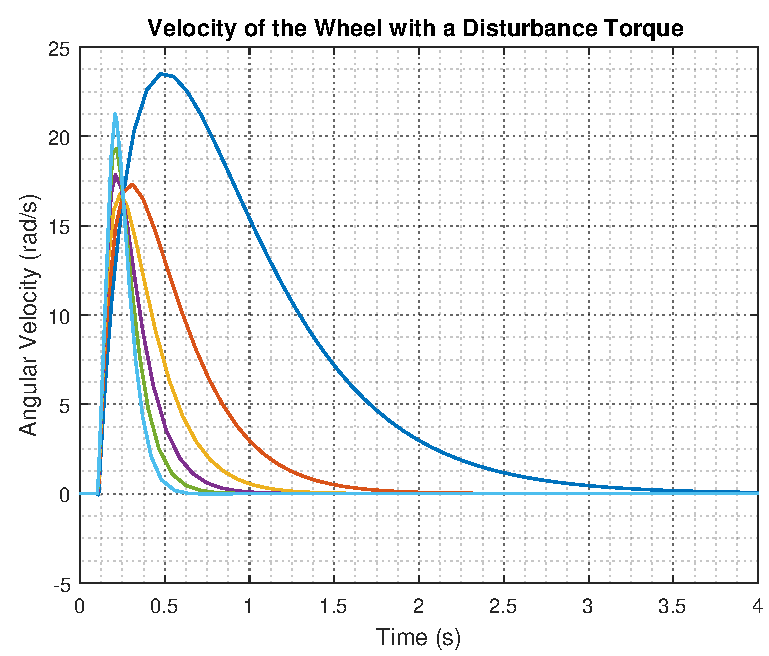
\includegraphics[scale=.55]{figures/disturbanceStateSpaceWheel}
			\centering
			\captionsetup{justification=centering}
			\captionof{figure}{Velocity of the wheel with the same disturbance}
			\label{disturbanceStateSpaceWheel}
		\end{figure}
	\end{minipage}
\end{minipage}
%
\begin{minipage}{\linewidth}
	\begin{minipage}{0.45\linewidth}
		\begin{figure}[H]
			\includegraphics[scale=.55]{figures/catchingStateSpace}
			\centering
			\captionsetup{justification=centering}
			\captionof{figure}{Response starting from \si{0,2\ rad} and an initial velocity of the wheel with different locations of poles}
			\label{catchingStateSpace}
		\end{figure}
	\end{minipage}
	\hspace{0.03\linewidth}
	\begin{minipage}{0.45\linewidth}
		\begin{figure}[H]\vspace{-3mm}
			\includegraphics[scale=.55]{figures/catchingStateSpaceWheel}
			\centering
			\captionsetup{justification=centering}
			\captionof{figure}{Velocity of the wheel in the same starting conditions}
			\label{catchingStateSpaceWheel}
		\end{figure}
	\end{minipage}
\end{minipage}

The final combination of poles is \si{-6}, \si{-7} and \si{-15}, which gives the yellow responses in \figref{disturbanceStateSpace} and \figref{catchingStateSpace}. This seems a good option since its response is quite fast but not with too much overshoot. It can also be observed that the velocity of the frame is in all the cases \si{0\ rad \cdot s^{-1}} The gain matrix for this combination results in the following:
%
\begin{equation}  \label{controllerSS}
	\vec{K} = 
	\begin{bmatrix}
		-2,3021 & -0,2274 & -0.0039 \\
	\end{bmatrix}
\end{equation}
%	%-------- Controller in State Space
	\section{State Space Controller Implementation}\label{sec:SSImplementation}
The controller in state space results to be three gains that do not need to be discretized to implement them in the real system. 
Contained in \lstinline{x_hat} are the states of the system being the angle of the frame (\lstinline{x_hat[0]}), the velocity of the frame (\lstinline{x_hat[1]}) and the velocity of the wheel (\lstinline{x_hat[2]}). \lstinline{x_hat} is the equivalent of vector \si{\vec{x}}. The inner product between \si{\vec{K}} and \si{\vec{x}} is calculated on line 11 in code listing \ref{codeStateSpaceControl}. On line 14 the found output torque is converted to a current, since the motor control board takes a current as reference. The \lstinline{TORQUE_2_CURRENT} constant is found by taken the inverse of the motor torque constant.
\begin{lstlisting}[caption  = {Code for the implementation of the State Space Controller. The feedback from the cubli is contained in the array x\_hat.},
label    = codeStateSpaceControl ]
/** Runs the controller based on the feedback signal in x_hat */
LSF_COutput_struct_T AAU3_DiscLinFeedback2(const real_T x_hat[3])
{
/** Variable declarations */
LSF_COutput_struct_T LSF_Sig_Out;

/** Controller calculations */
LSF_Controller.tau_m = 0;
for (int i = 0; i < 3; i++)
{
LSF_Controller.tau_m += LSF_Controller.K[i] * x_hat[i];
}

LSF_Sig_Out.I_m = LSF_Controller.tau_m * TORQUE_2_CURRENT;

return LSF_Sig_Out;
}
\end{lstlisting}
The important part of the implementation, and in some cases it can give problems, is the measurement of the states that are involved in the feedback.
In the case of the Cubli, there are three states to be measured: the position and velocity of the frame and the velocity of the wheel.

The first one can be measured using the values from the potentiometer or using built-in sensors like the IMU, as will be explained in detail in \chapref{chap:CompFilter}.

The velocity of the frame is measured using the gyroscopes present in both IMUs, which give an angular velocity value.

Finally, information about the velocity of the wheel is measured with a tachometer attached to the motor and send to the Beaglebone through the motor control board. 
\\
\begin{figure}[H]\vspace{-4mm}
	\centering
	\includegraphics[scale=.75]{figures/measurements}
	\captionof{figure}{Internal states measurements for the implementation of the controller}
	\label{fig:measurements}
\end{figure}\vspace{-5mm}
	%-------- Implementation of the Controller 
		
	%---------- Chapter 10 ----------------------------------------- Complementary Filter
	\chapter{Angle Measurement with Built-in Sensors}\label{chap:CompFilter}
It is a goal to get the Cubli setup to balance the frame in an upright position independently of the baseplate orientation within the possible angle of rotation.

As described in \secref{sec:Sensors} there are two IMUs mounted on the frame of the Cubli (shown on \figref{Cubli-6}). They can be used to achieve this goal since they only depend on the absolute angle and they can also be used in the full Cubli.

\section{Angle Calculations from the IMUs}
The angular position of the Cubli can be calculated using the accelerometer, the gyroscope or combining both. In this section each of the options is describe and analyzed.

\subsection{Angle from the Accelerometer}
The accelerometer measures linear acceleration, and if the accelerometer is attached to a object that does not accelerate with respect to the Earth, the accelerometer will measure the gravitational acceleration. This can be used to determine the orientation of the accelerometer sensor with respect to the Earth \cite{JWarren}.\\
The accelerometers used with the Cubli setup have 3-axis detection as described in \secref{sec:Sensors}. To determine the angle of the frame (\si{\theta_F}) with the accelerometer it is needed to get the measurements from two of the three axes. The two measurements needed are the ones in line with the frames movement direction, based on the way the IMU is mounted, as shown in \figref{accelerometer}. 
\begin{figure}[H]
	\centering
	\includegraphics[scale=0.58]{figures/accelerometer}
	\caption{Position of the IMU on the setup. The orientation of the accelerometer in relation to the Cubli frame is shown, which is rotated by \si{\frac{\pi}{4}} in relation to the angle \si{\theta_F}. On the IMU the components of the acceleration vector are shown. In case of no movement by the frame these are the components of the gravitational acceleration vector.}
	\label{accelerometer}
\end{figure}\vspace{-5mm}
%
Based on the markings on the IMU, those are the x- and y-axis components of the linear acceleration. Taking the two axis measurements shown in figure \ref{accelerometer} the angle can be found using \eqref{accelAngle} \cite{CFisher}. 
%
\begin{flalign}
	\eq{accel\_\theta_{F}} {\arctan\left(\frac{y}{x}\right) + \frac{\pi}{4}} \unit{rad} 
	\label{accelAngle}
\end{flalign}
%
\hspace{6mm} Where:\\
\begin{tabular}{ p{1cm} l l l}
	& x			& is the x component of the measured linear acceleration   & \unitWh{m \cdot s^{-2}} \\  
	& y			& is the y component of the measured linear acceleration   & \unitWh{m \cdot s^{-2}} \\ 	                     
\end{tabular} \\
\\
The offset (\si{\frac{\pi}{4}}) is added because the IMU is mounted with a \si{\frac{\pi}{4}} rotation compared to the orientation of the frame.\\
A test to measure the angle of the frame with the accelerometer is performed, and with the purpose to compare it to data from the potentiometer taken at the same time. The data from both sensors is read at the same time, to make it possible to compare the accelerometer to the potentiometer to determine if the accelerometer can be used instead of the potentiometer.\\
A comparison of the two measurements is shown in \figref{angleAcc}. The accelerometer angle (\si{accel\_\theta_{F}}) is found by taking the x- and y-axis components and calculating the angle with \eqref{accelAngle}.
The data from the test can be found in  \appref{app:IMUMeasurementsAppendix}. 
%
\begin{figure}[H]
	\centering
	\includegraphics[scale=0.65]{figures/angleAcc}
	\caption{The graph shows a comparison of the angle of the frame measured by the potentiometer(orange) and the same angle found with the accelerometer(blue). The accelerometer angle is calculated based on the measurement data from the x- and y-axis component (\appref{app:IMUMeasurementsAppendix})}
	\label{angleAcc}
\end{figure}\vspace{-5mm}
%
The measurements of the potentiometer and accelerometer are both showing the Cubli frame in the same position. The measurement from the accelerometer has a lot more noise than the potentiometer.\\
While the Cubli setup tries to balance the frame, the IMU mounted on the top of it will move along with the frame and the spikes seen on the calculated angle data from the accelerometer data in \figref{angleAcc} are because the IMU is moving and the acceleration from this creates a disturbance on the measurement of the gravitational acceleration \cite{JWarren}.\\
A way to minimize this disturbance would be to move the IMU as close as possible to the point of rotation. This way the accelerometer is still able to see the angle of the frame, but the distance it is moved is shorter and the acceleration will be smaller. \fxnote{we didnt do this because we would have to remount the sensor and create a new mount. how to best word that?, B}

\subsection{Angle from the Gyroscope}
The angle of the frame can be found with the gyroscope by integrating the angular velocity measured by the gyroscope on the axis aligned with the direction of motion of the frame as shown in \figref{cubliMechanical}.
\begin{flalign}
	\eq{gyro\_\theta_{F}[n]} {\int_{0}^{n\cdot \Delta T} \omega_{F} \, \mathrm{d}t}
	\label{accelGyro}
\end{flalign}
\hspace{6mm} Where:\\
\begin{tabular}{ p{1cm} l l l}
	& \si{\omega_{F}}			& is the measured angular velocity of the frame  & \unitWh{rad \cdot s^{-1}} \\  \\                       
\end{tabular} 
\\
The problem with the data from the gyro is an accumulating error which is caused by the integration done to convert angular velocity into an usable angle. It is also known that the gyros will exhibit a drifting error when experiencing small and slow movement \cite{JWarren}. These problems can be observed in \figref{angleGyro}.
\begin{figure}[H]
	\centering
	\includegraphics[scale=0.65]{figures/angleGyro}
	\caption{Angular position calculation with the data of the gyroscope}
	\label{angleGyro}
\end{figure}\vspace{-5mm}
%The problem with the data from the gyro is it will exhibit a drifting error when experiencing no movement \cite{JWarren} and since the angular velocity has to be integrated to get the angel there will be an accumulation error. 

Assuming that the drift is proportional to time (the slope is always constant), a way to minimize its influence on the data would be to do a test while keeping the frame motionless. The inclination of the slope from the data graph multiplied with the sampling time is then the offset that has to be subtracted from each measurement.

It can also be calculated online, while the controller is running. In this case the accelerometer can provide information to compensate this drift. One solution to fuse these two sets of data is to use a complementary filter, explained in detailed in next section.

\subsection{Data Fusing with Complementary Filter}
In order to filter the drift of the gyroscope and the disturbance errors of the accelerometer a complementary filter can be used to combine both measurements from the IMU mounted on the Cubli frame. This is done with the goal to get a more reliable angle measurement for both when the frame is moving and when its standing still in the equilibrium point.\\
The two angle measurements of the IMU are sent through a filter and then summed in order to get an angle of the Cubli's frame. When the frame is moving fast it is better to rely on the gyroscope data, and when the frame is moving slowly or not at all it is better to rely on the accelerometer data \cite{PGui}.

\begin{figure}[H]
	\begin{tikzpicture}[ auto,
thick,                         %<--setting line style
node distance=2cm,             %<--setting default node distance
scale=1.5,                     %<--|these two scale the whole thing
every node/.style={scale=1.5}, %<  |(always change both)
>=triangle 45 ]                %<--sets the arrowtype
\draw%--------------------------------------------------------------------------------------------

node[shape=coordinate][](acc) at (0,0){acc}			% start of acc signal path

node(lowpas) at (6,0) [block] {\Large $\ \frac{1}{\tau \cdot s + 1}$ }

node[shape=coordinate][](gyro) at (0,-2){}		% start of gyro signal path

node(integrate) at (3,-2) [block] {\Large $\frac{1}{s}$}

node(highpas) at (6,-2) [block] {\Large $\ \frac{\tau \cdot s}{\tau \cdot s + 1}$ }

node(sum) at (8,-1) [sum] {$\sum$}


node[shape=coordinate][](angle) at (10,-1){}		% output of the complementary filter
;

\draw[->](acc) -- node {accel$\_\theta_{F}$} (lowpas);
\draw[->](gyro) -- node {gyro$\_\omega_{F}$} (integrate);
\draw[->](integrate) -- node {} (highpas);

\draw[->](highpas) -| node {} (sum);
\draw[->](lowpas) -| node {} (sum);


\draw[->](sum) -- node {$\theta_{F}$} (angle);

\end{tikzpicture}

	\centering
	\caption{Block diagram of the complementary filter setup used with the IMU on the Cubli. The calculated accelerometer angle gets passed through a low pas filter. The angular velocity measurement from the gyro is integrated and then passed through a high pas filter. Both measurements are then summed to get the angle of the frame.}
	\label{blockDrawingComplementaryFilter}
\end{figure}

The filter for the IMU is designed as shown in \figref{blockDrawingComplementaryFilter} with a low pass filter on the measurements from the accelerometer, and an integration followed by a high pass filter on the measurements from the gyroscope \cite{OlliW}. \cite{PGui}
\begin{flalign}
	\eq{\theta_{F}} {\frac{1}{ 1 + \tau \cdot s} \cdot accel\_\theta_{F}}   &\\
	\eq{\theta_{F}} {\frac{\tau \cdot s}{ 1 + \tau \cdot s} \cdot \frac{1}{s} \cdot gyro\_\dot{\theta}_{F}}	&
	\label{complementaryBlockFilters}
\end{flalign}
Combining the two equations yields \eqref{complementaryCombinedFilter}
\begin{flalign}
	\eq{\theta_{F}} {\frac{1}{ 1 + \tau \cdot s} \cdot accel\_\theta_{F} + \frac{\tau \cdot s}{ 1 + \tau \cdot s} \cdot \frac{1}{s} \cdot gyro\_\dot{\theta}_{F} = \frac{accel\_\theta_{F} + \tau \cdot gyro\_\dot{\theta}_{F}}{1 + \tau \cdot s}} &
	\label{complementaryCombinedFilter}
\end{flalign}
The \si{\tau} is the cut-off frequency of the two filters. Changing this constant decides how much the two different sensor measurements weight in on the combined angle.
 
\section{Discretization of the Complementary Filter} 
In oder to use the complementary filter on the Cubli it needs to be discretized. This is done with the bilinear transformation method where \si{s = \frac{2}{\Delta T}\cdot \frac{1 - z^{-1}}{1 + z^{-1}}}, with a sample time of \SI{10}{ms}.
Rewriting \eqref{complementaryCombinedFilter} yields
\begin{flalign}
 	\eq{\theta_{F}} {\frac{1}{1 + \tau \cdot s} \cdot (accel\_\theta_{F} + \tau \cdot gyro\_\dot{\theta}_{F})} &
 	\label{discreteComplementaryFilter1}
\end{flalign}
If s is replaced by its discrete expression, the difference equation can be derived.
\begin{flalign}
  	\eq{\theta_{F}} {\frac{1}{1 + \tau \cdot \frac{2}{\Delta T}\cdot \frac{1 - z^{-1}}{1 + z^{-1}}} \cdot (accel\_\theta_{F} + \tau \cdot gyro\_\dot{\theta}_{F})} &
  	\label{discreteComplementaryFilter2}
\end{flalign}
%
%\begin{flalign}
%  	\eq{\Updownarrow \theta_{F}} {\frac{\Delta T \cdot (1 + z^{-1})}{\Delta T \cdot (1 + z^{-1})+2\cdot (1 - z^{-1})\cdot \tau} \cdot (accel\_\theta_{F} + \tau \cdot gyro\_\dot{\theta}_{F})}
%  	\label{discreteComplementaryFilter3}
%\end{flalign}
  %
\begin{flalign}
   	\eq{\theta_{F}} {\frac{\Delta T + \Delta T \cdot z^{-1}}{(2\cdot \tau + \Delta T) - (2\tau - \Delta T)\cdot z^{-1}} \cdot (accel\_\theta_{F} + \tau \cdot gyro\_\dot{\theta}_{F})} &
\end{flalign}\label{discreteComplementaryFilter4}
%
%\begin{flalign}
%	\eq{\Updownarrow \theta_{F} \cdot ((2\cdot \tau + \Delta T) - (2\tau - \Delta T)\cdot z^{-1})} {\Delta T + \Delta T \cdot z^{-1} \cdot (accel\_\theta_{F} + \tau \cdot gyro\_\dot{\theta}_{F})} &
%\end{flalign}\label{discreteComplementaryFilter5}
%%
Now \eqref{discreteComplementaryFilter4} is transformed from z-domain to discrete time domain. Which gives us \eqref{discreteComplementaryFilter7}.
% OLD 9.9
%\begin{flalign}
%	\eqOne{\theta_{F}[n] \cdot (2\cdot \tau + \Delta T) - \theta_{F}[n-1] \cdot (2\tau - \Delta T)} {\Delta T \cdot (accel\_\theta_{F}[n] + accel\_\theta_{F}[n-1]} 
%	\eqTwo{ + \tau \cdot gyro\_\dot{\theta}_{F}[n] + \tau \cdot gyro\_\dot{\theta}_{F}[n+1])} 
%	\label{discreteComplementaryFilter6}
%\end{flalign}
%  
\begin{flalign}
	\eqOne{\theta_{F}[n]}{\frac{(2\cdot \tau + \Delta T)}{2\cdot \tau + \Delta } \cdot \theta_{F}[n-1] + \frac{\Delta T}{2\cdot \tau + \Delta T} \cdot accel\_\theta_{F}[n] + \frac{\Delta T}{2\cdot \tau + \Delta T} \cdot accel\_\theta_{F}[n-1]} 
	\eqTwo{ + \frac{\Delta T \cdot \tau}{2\cdot \tau + \Delta T} \cdot gyro\_\dot{\theta}_{F}[n] + \frac{\Delta T \cdot \tau}{2\cdot \tau + \Delta T} \cdot gyro\_\dot{\theta}_{F}[n-1]} 
	\label{discreteComplementaryFilter7}
\end{flalign}
%

Implementing \eqref{discreteComplementaryFilter7} yields to following piece of code. \fxnote{USE the current form in the controller code file}

\begin{lstlisting}[caption  = {Code for the implementation of the complementary filter in C\texttt{++}. The comp\_angle[0] is the newest found angle of the frame.},
label    = codeCompFilter ]
//---------------------- IMU --------------------------//

const double acc_off = 0.84;  	// accel meass offset
const double tau = 0.5399;	// cut-off for the complementary filter

static double acc_angle[2]={atan(accY1/accX1) + acc_off,0},
gyro_angle[2]={gyroRads1,gyroRads1},
comp_angle[2]={acc_angle[0],0};

// Set old measurement data
acc_angle[1] = acc_angle[0];
gyro_angle[1] = gyro_angle[0];
gyro_angle[0] = gyroRads1;
comp_angle[1] = comp_angle[0];

// Get angle from accel axis measurements
acc_angle[0] = atan(accY1/accX1) + acc_off;

//Complementary equation using Tustin
const double K1 = (2*tau-Ts)/(2*tau+Ts);
const double K2 = Ts/(2*tau + Ts);
comp_angle[0] = K1*comp_angle[1] + K2*(acc_angle[0] + acc_angle[1] + tau*gyro_angle[0] + tau*gyro_angle[1]);
\end{lstlisting}
The offset for the accelerometer measurement and the cut-off frequency of the filter are defined as constants. When the controller start up it initializes the accel array and the gyro array with data pulled from the sensor. The initial complementary angle is set to be what the accelerometer measures.\\
The old values from accel\_angle, gyro\_angle and comp\_angle are moved up in their arrays and new data is saved in gyro\_angle and accel\_angle on index 0. The accel\_angle value is calculated from the x and y components.
The constants K1 and K2 are calculated from the sampling time and the set cut-off frequency. They are used in the complimentary filter.\\
The complimentary filter takes the new measurements from accelerometer and gyroscope and sums it with the previous measurements. The new calculated angle is then again summed with the old calculated angle.

\section{Calculation of the Cut-off Frequency}
Based on the setup of the complementary filter as seen in \figref{blockDrawingComplementaryFilter} the same cut-off frequency is chosen for both low and high pass filter, since it is desired to find the angle of the frame with a gain of 1.
%
\begin{figure}[H]
	\centering
	\includegraphics[scale=0.7]{figures/bodeFilters}
	\caption{Bode diagrams of the high pass and low pass filters as well as the summation of both}
	\label{bodeFilters}
\end{figure}\vspace{-5mm}
%
The cut-off frequency for the filters can be determined by using Senstools and the data obtained through the test detailed in \appref{app:IMUMeasurementsAppendix}.

The toolbox uses the data form the potentiometer as the real output of the system, the data from the IMUs as the input and the modeling of the system is done through \eqref{discreteComplementaryFilter7}. With this data Senstools can find the optimal value for \si{\tau} based on the difference between the angle measured by the potentiometer and an angle calculated from accelerometer and gyroscope measurements done during the same test.

The final fit can be seen in \figref{filterSensTool} and it gives an optimal \si{\tau\ =\ 0,5399}. This results in a cutting frequency for the filter equal to \si{1,85\ rad \cdot s^{-1}}.

%
\begin{figure}[H]
	\centering
	\includegraphics[scale=0.65]{figures/filterSensTool}
	\caption{Final result of the complementary filter compared with the data from the potentiometer}
	\label{filterSensTool}
\end{figure}\vspace{-5mm}
%
Using the same cut-off frequency for both filters has been sucessfully implemented and hence it there was not done any investigation into different cut-off frequencies for the low and high pass filter.\\
		
	
	%%% Part 3 %%%
	\part{Test \& Conclusion}
	\chapter{Acceptance Test}
This chapter deals with the needed tests that the system must overcome in order to fulfill the requirements as well as an analysis of the other capabilities, described in \chapref{chap:specifications}.

\section{Requirements Test}

- \textbf{The Cubli should be able to balance starting from an unstable equilibrium position and null velocity.}

To test this requirement, the Cubli is placed at equilibrium and the controller is then started. The test is done twice, first with the measurements of the potentiometer andthen using the IMU, to ensure that the controller works in both cases.

\begin{minipage}{\linewidth}
	\begin{minipage}{0.45\linewidth}
		\begin{figure}[H]
			\includegraphics[scale=.45]{figures/testReq1}
			\centering
			\captionsetup{justification=centering}
			\captionof{figure}{Angular position of the frame, measured with the potentiometer, when starting from equilibrium position.}
			\label{testReq1}
		\end{figure}
	\end{minipage}
	\hspace{0.03\linewidth}
	\begin{minipage}{0.45\linewidth}
		\begin{figure}[H]\vspace{0mm}
			\includegraphics[scale=.45]{figures/testReq1_IMU}
			\centering
			\captionsetup{justification=centering}
			\captionof{figure}{Angular position of the frame starting from equilibrium position, calculated with the complementary filter.}
			\label{testReq1_IMU}
		\end{figure}
	\end{minipage}
\end{minipage}
%

The results show that the requirement is fulfilled in both cases since the system is maintained around the equilibrium position.

- \textbf{The prototype should be able to balance around \si{0\ \rad}, even though the angle of inclination of the baseplate is changed within a reasonable range, using internally mounted sensors.}

To check this requirement a similar test, like the previous one, is done, but is this case the angle of the baseplate is changed to check that the measurements of the IMU are still capable of balance the Cubli. Since the potentiometer is attached to the baseplate its measurements are done in relation to the baseplate's position and can be used to show that baseplate and frame are at different angles.

\begin{figure}[H]
	\centering
	\includegraphics[scale=0.62]{figures/testReq2}
	\caption{Angular position of the frame. The orange curve is the result of the complementary filters angle calculation, which does not depend on the angle of the baseplate. The blue curve shows the measurements of the potentiometer, which are in relation to the baseplate.}
	\label{testReq2}
\end{figure}\vspace{-5mm}
%
The output of this experiment shows that the calculation of the position using the IMU makes the system able to keep in equilibrium position when the angle of the Baseplate is changed. This can be seen on the graph in \figref{testReq2}. Here the angle calculated by the complementary filter shows the frame keeping its upright position, while the potentiometer angle changes as the baseplate is lifted up and down. 

\section{Capabilities Analysis}
- \textbf{Maximum recovery angle}

To obtain the maximum recovery angle, the Cubli is place in equilibrium at the start. Once the controller has balance it, its position is changed with little disturbances. The result can be seen in \figref{testRecovery}.

\begin{figure}[H]
	\centering
	\includegraphics[scale=0.62]{figures/testRecovery}
	\caption{Angular position of the frame while disturbances are applied to the frame. The intention is to find the maximum recovery angle of the controller. The controller is not able to recover from a disturbance that pushes the frame over \SI{0,08}{rad} from resting position, due to the overshoot.}
	\label{testRecovery}
\end{figure}\vspace{-5mm}
%
As it can be observed, the controller is able to return to equilibrium position but it creates a remarkable overshoot in the other direction. This behavior limits the recovery angle since the overshoot may drive the Cubli to an angle beyond its handling limit even though the initial disturbance is within it.\\
It can be seen that the controller is capable of recovering from \si{0,08\ rad} but it fails when the angle is \si{0,1\ rad}. Then, it can be concluded that the maximum recovery angle for the system with the designed controller is \si{0,08\ rad}.

- \textbf{Maximum catching angle with no initial velocity of the wheel}

There exists a limitation in this capability which is given by the maximum current that the motor can provide. As can be seen in \figref{limitationTorque}, if the initial angle is different from 0 rad both the mass of the frame and the mass of the wheel exert an initial torque to the system. This must be overcame by the motor to avoid the Cubli to fall.

\begin{figure}[H] 
	\centering
	\includegraphics[scale=0.65]{figures/limitationTorque}
	\caption{Forces acting on the system that create an initial torque when the frame starts from a position different from 0 rad}
	\label{limitationTorque}
\end{figure}

The minimum torque (T) that the motor must apply is give by \eqref{minTorque}.
%
\begin{flalign}
	\eq{T} { (m_F \cdot l_F + m_w \cdot l_w) \cdot g \cdot sin(\theta_F)} \unit{N\cdot m}
	\label{minTorque}
\end{flalign}

Since the torque is restricted by the characteristics of the motor and the control board, the maximum initial angle is derived in \eqref{maxAngle}.
%
\begin{flalign}
	\eq{\theta_F} { asin\left(\frac{T}{(m_F \cdot l_F + m_w \cdot l_w) \cdot g}\right)} \unit{rad}
	\label{maxAngle}
\end{flalign}
%
Substituting the values of the maximum torque (see section \secref{sec:Motor}) and the parameters of the Cubli (see section \secref{sec:Param}) the maximum possible starting angle is \si{0,2024\ rad} (\si{11,59^\circ}). This also applies for the negative angle since the limitation of torque is the same but with opposite sign. 

Taking this limit into account some starting angles are tested to check if the controller is able to balance the system with these initial conditions. 

As it can be seen in \figref{testCatch_12} and \figref{testCatch_17}, the controller is capable of moving the system to equilibrium position starting from \SI{-0,12}{rad} and \SI{-0,17}{rad} (also valid for the positive angles). It is also noteworthy that as the starting angles goes away from the equilibrium the controller takes more time and there is more oscillations in the response.

\begin{minipage}{\linewidth}
	\begin{minipage}{0.45\linewidth}
		\begin{figure}[H]
			\includegraphics[scale=.55]{figures/testCatch_12}
			\centering
			\captionsetup{justification=centering}
			\captionof{figure}{Angular position of the frame when the system starts from \SI{-0,12}{rad} (\si{-6,87^\circ})}
			\label{testCatch_12}
		\end{figure}
	\end{minipage}
	\hspace{0.03\linewidth}
	\begin{minipage}{0.45\linewidth}
		\begin{figure}[H]\vspace{-3mm}
			\includegraphics[scale=.55]{figures/testCatch_17}
			\centering
			\captionsetup{justification=centering}
			\captionof{figure}{Angular position of the frame when it starts from \SI{-0,17}{rad} rad (\si{-9,74^\circ})}
			\label{testCatch_17}
		\end{figure}
	\end{minipage}
\end{minipage}

However, when the starting angle is \SI{-0,185}{rad} (\si{-10,59^\circ}) is no longer possible to balance the system in equilibrium position and the frame falls.

\begin{figure}[H] 
	\centering
	\includegraphics[scale=0.55]{figures/testCatch_185}
	\caption{Angular position of the frame when it starts from \SI{-0,185}{rad} (\si{-10,59^\circ})}
	\label{testCatch_185}
\end{figure}
%
It can be concluded that the maximum range for the starting angle with zero initial conditions goes from \SI{-0,17}{rad} to \SI{-0,17}{rad}, in which the controller is able to balance the system around equilibrium position.
	\chapter{Discussion}
Some decisions made throughout the course of the project are discussed in this chapter. 
%The performance of the one sided system can be by just looking at it as reaction wheel inverted pendulum.

For the state space controller a set of poles were selected looking at the response they showed in the two simulations, \figref{catchingStateSpace} and \figref{catchingStateSpaceWheel}. Using different pole combinations results in different overshoots and settling time, so another pole combination could be selected if a different behavior of the Cubli was desired. 
The choice is whether a small overshoot is desired or if the frame is to reach \SI{0}{rad} faster. 
Having less overshoot would increase the maximum catching angle with the current system, since the second overshoot with the current used controller is larger than the angle inflicted by a disturbance. 
Braking the wheel faster gives the controller more acceleration to use in order to counteract a disturbance. \fxnote{rephrase the "more accel" thing}

As already mentioned briefly in the complementary filter section, the measurement from the accelerometer in the IMU could be improved by moving the sensor to a position where it would be influenced less by the acceleration of the frame but still be able to measure the angle of the frame. In case of the single frame, that would be as close as possible to the point of rotation fixed to the baseplate.

The combining of accelerometer and gyroscope measurement can be done using a different type of filter than the used complementary filter. The decision to use the complementary filter was based on the usage of it in similar applications \cite{OlliW}. Since it shows a good behavior for the problem at hand and no further investigation was needed.

%{\Large notes} \fxnote{delete this part its just to brainstorm what to write in this section}\\
%- Placement of IMU\\
%- Choice of Statspace variables for controller - minimize overshoot vs faster braking for wheel\\
%- cut-off frequency of the complementary filter?\\
%- code accessibility?\\
%- classical controller?\\
%

%As already mentioned briefly in the complementary filter section, the measurement from the accelerometer in the IMU could be improved by moving the sensor to a position where it would be influenced less by the acceleration of the frame but still be able to measure the angle of the frame. 

%For the state space controller a set of poles were selected looking at the response they showed in the two simulations, \figref{catchingStateSpace} and \figref{catchingStateSpaceWheel}. Using different pole combinations results in different overshoots and settling time, so another pole combination could be selected if a different behavior of the Cubli was desired. 
%The choice is whether a small overshoot is desired or if the frame is to reach \SI{0}{rad} faster. 
%Having less overshoot would increase the maximum catching angle with the current system, since the second overshoot with the current used controller is larger than the angle inflicted by a disturbance. 
%Braking the wheel faster gives the controller more acceleration to use in order to counteract a disturbance. \fxnote{rephrase the "more accel" thing}
%\\-\\
%The classical controller designed and implemented was a single-input single-output system controller (SISO). A frequency design could maybe be done with multiple inputs and multiple controllers. It cannot be a cascaded design as that has been said to be impossible. \fxnote{if this is kept, reference that paper on this topic again}
%\\-\\
%The controller designed in this project can only keep the frame upright at the equilibrium position. It will not be possible to keep the frame at an angle different than \si{0^\circ} because the wheel cannot accelerate unlimited. Changing the restrictions that are on system might mean replacing a few components like the motor control board. Giving the motor a higher speed ceiling allows ths system to accelerate longer or accelerate faster to generate more torque. The longer the wheel can keep accelerating the longer will be able to keep the frame a position different from \si{0^\circ}.
%\\-\\
%The Inertia of the reaction wheel could be changed. this could be done by changing its size and/or its mass. Assuming the same torque is wanted a larger inertia means a slower acceleration is needed to generate the torque. The larger inertia also means slower response time. A wheel with smaller inertia would have to accelerate faster to generate the same torque, but it would also have a faster response time. \fxnote{somebody double check my assumption about physics} The inertia of the wheel could be something that could be optimized, depending on what is needed for the rest of the system. More torque or faster response time.
%\\-\\

	\chapter{Conclusion}

The aim of this project was to work with an unstable nonlinear system and be able to construct an appropriate model and design a controller capable of balancing it around equilibrium position.

First, a pre-analysis of the system has been made, starting from a description of all the components present in the given setup. It also included the derivation of the equations that describe the dynamics and the description of the system in s-domain. Then the parameters of the setup have been found, both with measurements and with an estimation using optimization, to be able to analyze the behavior of the system and compare it with the real model.

Afterwards, a controller has been designed to balance the Cubli in upright position using root locus. It has been shown necessary to control both the angular position of the frame and the velocity of the wheel so it was decided to use a state space approach.

It was also a requirement to be able to change the angle of the baseplate, which means that the calculation of the angle had to be independent of the inclination. A very convenient option was to use built-in sensors for this purpose, so the final chosen solution was to use an IMU present on the setup and calculate the angle through a complementary filter.

Finally, some acceptance tests have been performed to ensure that the final controlled system was able to accomplish the requirements and, similarly, a further analysis has been carried out to check other capabilities of the Cubli.

In conclusion, a control system that can balance the Cubli in upright position independently of the angle of the baseplate, within a reasonable range, has been designed, implemented and tested successfully within the requirements.



	\chapter{Perspective}

In the state space controller a set of poles were selected looking at the response they showed in two simulations, \figref{catchingStateSpace} and \figref{catchingStateSpaceWheel}. Using different pole combinations results in different overshoots and settling time, so another pole combination could be selected if a different behavior of the Cubli was desired. The choice is whether a small overshoot is desired or if the frame is to reach \SI{0}{rad} faster.

One of the next steps will be to build the full Cubli, since now the control can be done using only components attached to the frame. This design needs to include the control of three reaction wheels to control each of the directions that the full Cubli could move in.

The Cubli will have to be able to jump up from a resting position. To do that the reaction wheel has to spin up. Once at the desired speed the wheel will be braked and the resulting torque will raise the Cubli. Now the system has to catch itself. In order to do that a separate controller might have to be designed that handles the jump up part, and then switches to the balancing controller for the position keeping part.\\
For the full Cubli there will be 3 brakes, one on each wheel, that have to be coordinated to raise the cube up to a desired position.
%This new configuration may also need the system to be able to jump up from resting position and then the brake system must be taken into account for each of the wheels. 

It is possible that the controller no longer needs to balance each of them in upright position but to do another kind of maneuvers, which will require a new controller since the chosen one is not able to get a reference for the internal states different from zero.


- Jump up\\
- 3D Cube\\
- Deep more in other possibilities of controllers\\
- May not need to balance, but to do another maneuvers -----> other controller -----> same model\\
- Show and advertise control engineering \\
	
	%%% Setup for Appendix and Bibliography %%%
	\bookmarksetup{startatroot}
	\addtocontents{toc}{\bigskip}
	\newpage
	\fancyhead[RO]{\color{aaublue}\small Appendix \nouppercase\rightmark} %even page - chapter title
	\fancyhead[LE]{\color{aaublue}\small Appendix \nouppercase\rightmark} %uneven page - section title
	\fancyhead[RE,LO]{}
	\titleformat{\section}[hang]{\Large\bfseries}{\thesection\hsp\textcolor{aaublue}{|}\hsp}{0pt}{\Large\bfseries}

	%%% Appendix %%%
		%\renewcommand{\thechapter}{\Alph{chapter}}
		%	\addcontentsline{toc}{chapter}{Appendix}
		%	\setcounter{chapter}{0}
		%	\setcounter{section}{0}
		%	\setcounter{table}{0}
		%	\setcounter{equation}{0}
		%	\setcounter{figure}{0}
	\appendix
	
	\part*{Appendix}
	\addcontentsline{toc}{chapter}{Appendix}	
		
	%---------- Appendix A ---------------------------------------- 
	\chapter{Potentiometer Angle Resolution}\label{app:potentiometerRes} 
\textbf{Name: Group 630}\\
\textbf{Date: 15/03 - 2016}

\subsubsection{Purpose}
Finding the resolution needed for the conversion of potentiometer voltage to angles, along with possible offsets.

\subsubsection{Setup}
\begin{figure}[H]
  \centering
	\includegraphics[scale=1]{figures/LabSetupRangeTest.pdf}
	\caption{Setup diagram}
	\label{LabSetupRangeTest2}
\end{figure}\vspace{-5mm}

\subsubsection{List of Equipment}
\begin{table}[H]
	\begin{tabular}{|l|l|p{4.3cm}|}
		\hline%------------------------------------------------------------------------------------------------------------
		\textbf{Instrument}                                  &  \textbf{AAU-no.}  &  \textbf{Type}                       \\
		\hline%------------------------------------------------------------------------------------------------------------
		Oscilloscope                                         &  61604             &  Agilent 54621A		                   \\
		\hline%------------------------------------------------------------------------------------------------------------
		Dedicated Power Supply of Cubli \small{(24 V - 3 A)} &                    &  XP Power, AEB70US24                 \\
		\hline%------------------------------------------------------------------------------------------------------------
		Probe                                          &                &   1:1   \\
		\hline%------------------------------------------------------------------------------------------------------------
	\end{tabular}
\end{table}

\subsubsection{Procedure}
\begin{enumerate}
  \item Make the setup with connections as seen on \figref{LabSetupRangeTest}, with ground on the brown cable and signal on yellow cable of the potentiometer.
  \item Set the oscilloscope on rolling and calibrate so that the full range of the frame movement can be captured on the display.
  \item Balance the frame in upright equilibrium position.
	\item Move the frame to the left position, hold for a brief duration, then move it over to the right position.
	\item Once both the equilibrium, leftmost and rightmost positions are captured on the screen, pushing the stop-button on the scope, to hold keep the measurement.
	\item Save the data to the floppy-disk as a CSV file.
\end{enumerate}

\subsubsection{Results}
\begin{figure}[H] 
	\centering 
	\includegraphics[scale=0.7]{figures/TestPotentiometerResolution}
	\caption{Raw test data plot, Volt over time}
	\label{comparisonRealModel}
\end{figure}
	
	%---------- Appendix B ---------------------------------------- 
	\chapter{Fall Response}\label{fallResponseAppendix} 
\textbf{Name: Group 630}\\
\textbf{Date: 17/03 - 2016}

\subsubsection{Purpose}
Find the fall response of the frame from the vertical position, \si{\theta_F=0}\fxnote{might change depending on what is decided as the "real" 0 because of potmeter offset}, and from a \si{10^\circ}\fxnote{Might chance depending on data } tilted position.
Data is used to compare the measured response and the simulation given by the theoretical nonlinear model.


\subsubsection{Setup}
The wheel is being held in a fixed position with a strip tied to it and the frame. The probe chosen is a 1:1 and is connected to the potentiometer with probe to yellow cable and ground clamp to brown cable. The power supply has to be turned on in order to get readouts from the potentiometer. A sponge is placed on the rubber pad in order to damp the impact of the frame.
\begin{figure}[H]                                   
	\centering                                        
	\includegraphics[scale=0.08]{figures/stepResponseSetup}
	\caption{Picture of the setup for the fall-response test}
	\label{stepResponseTestPicture} 
\end{figure}              

\subsubsection{List of Equipment}
\begin{table}[H]
	\begin{tabular}{|l|l|p{4cm}|}
		\hline%------------------------------------------------------------------------------------
		\textbf{Instrument}                        &  \textbf{AAU-no.}  &  \textbf{Type}       \\
		\hline%------------------------------------------------------------------------------------
		Cubli setup                              &               &  		  \\
		\hline%------------------------------------------------------------------------------------
		Oscilloscope                              &  61604             &  Agilent 54621A		  \\
		\hline%------------------------------------------------------------------------------------
		Dedicated Power Supply of Cubli \small{(24 V - 3 A)} &               &  XP Power, AEB70US24 \\
		\hline%------------------------------------------------------------------------------------
		Probe 1:1                &  TBD            &          TBD   \\
		\hline%------------------------------------------------------------------------------------
		Sponge               & 5P0N63             &              \\
		\hline%------------------------------------------------------------------------------------
	\end{tabular}
\end{table}
fix of table\fxnote{find the probe used} 
\subsubsection{Procedure}
\begin{enumerate}
	%\item Turn on the power supply
	\item Keep the Cubli in the starting position (\si{0^\circ} or \si{10^\circ})
	\item Let the Cubli fall over
	\item Use the oscilloscope to measure the voltage changes in the potentiometer and save them
	\item Take the measurements and plot them in Matlab
	%\item Plot the result of the simulations in the same figure and compare them
\end{enumerate}


\subsubsection{Results}
Data from the test is presented in a graph showing the voltage measured, and in a graph with the voltage converted to radians.
The data is available as a .csv file on the CD\fxnote{Make sure this is put into the CD folder for copying}

\small\textbf{Fall response starting from \si{0^\circ}}

\begin{minipage}{\linewidth}
	\begin{minipage}{0.45\linewidth}
		\begin{figure}[H]
			\includegraphics[scale=.53]{figures/FallVolt}
			\centering
			\vspace{-.4cm}
			\captionsetup{justification=centering}
			\captionof{figure}{Raw data taken from the potentiometer}
			\label{FallVolt}
		\end{figure}\vspace{-5mm}
	\end{minipage}
	\hspace{0.03\linewidth}
	\begin{minipage}{0.45\linewidth}
		\begin{figure}[H]
			\includegraphics[scale=.53]{figures/FallRad}
			\centering
			\vspace{-.4cm}
			\captionsetup{justification=centering}
			\captionof{figure}{Angular position of the frame}
			\label{FallRad}
		\end{figure}\vspace{-5mm}
	\end{minipage}
\end{minipage} \fxnote{Look at the layout of picture of data placement}

\small\textbf{Fall response starting from \si{10^\circ}}

\begin{minipage}{\linewidth}
	\begin{minipage}{0.45\linewidth}
		\begin{figure}[H]
			\includegraphics[scale=.53]{figures/tenDegFallVolt}
			\centering
			\vspace{-.4cm}
			\captionsetup{justification=centering}
			\captionof{figure}{Raw data taken from the potentiometer}
			\label{tenDegFallVolt}
		\end{figure}\vspace{-5mm}
	\end{minipage}
	\hspace{0.03\linewidth}
	\begin{minipage}{0.45\linewidth}
		\begin{figure}[H]

			\includegraphics[scale=.53]{figures/tenDegFallRad}
			\centering
			\vspace{-.4cm}
			\captionsetup{justification=centering}
			\captionof{figure}{Angular position of the frame}
			\label{tenDegFallRad}
		\end{figure}\vspace{-5mm}
	\end{minipage}
\end{minipage} \fxnote{Look at the layout of picture of data placement}
fix\fxnote{link the correct pictures for the 0 degree experiment}


%The result of the experiment (\figref{comparisonRealModel}) shows that the response of the real system has several differences with the one from the simulation.
%
%The fist one is the presence of oscillations in the real response curve. This behavior is due to a small bounce that the frame does when it reaches the base.
%
%Another one is the final position of the frame, but it is due to the existence of a piece of foam at this position in the real case (to avoid the Cubli to hit the base).
%
%The other main difference is the shape of the curve, since the simulation is slower than the real case.

\subsubsection{Note}

There can be observed some bouncing in the data when the frame reaches the lower position due to the presence of the sponge.
Because of the sponge used as a cushion, to dampen the impact of the Cubli, there can be observed some bouncing in the data when the frame reaches the outer position.

The conversion from voltage to radians is based upon the test done in appendix X\fxnote{ADD reference to potentiometer test and the math behind the scaling}




	
	%----------Appendix C ---------------------------------------- 
	\chapter{Pendulum Behavior Test}\label{app:impulseResponseAppendix} 

\textbf{Name: Group 630}\\
\textbf{Date: 16/03 - 2016}

\subsubsection{Purpose}
Observe the behavior of the Cubli when hanging upside down. Data is then used to estimate some of the parameters of the Cubli.

\subsubsection{Setup}
The Cubli is put upside down under a table with 2 clamps placed at each side of the bottom plate of the Cubli setup.
The wheel is being held in a fixed position with a strip tied to it and the frame. The probe chosen is a 1:1 and is connected to the potentiometer with probe to yellow cable and ground clamp to brown cable. The power supply has to be connected, and turned on, to the Cubli in order to get readouts from the potentiometer.
\begin{figure}[H] 
	\centering 
	\includegraphics[scale=0.065]{figures/impulseResponseSetup}
	\caption{The Cubli setup hanging upside down beneath a table during the impulse response test}
	\label{impulseResponseTestPicture}
\end{figure} 

\subsubsection{List of Equipment}
\begin{table}[H]
	\begin{tabular}{|l|l|p{4.3cm}|}
		\hline%------------------------------------------------------------------------------------
		\textbf{Instrument}                        &  \textbf{AAU-no.}  &  \textbf{Type}       \\
		\hline%------------------------------------------------------------------------------------
		Cubli setup                              &               &  		  					\\
		\hline%------------------------------------------------------------------------------------
		Oscilloscope                              &  61604             &  Agilent 54621A		  \\
		\hline%------------------------------------------------------------------------------------
		Dedicated Power Supply of Cubli \small{(24 V - 3 A)} &               &  XP Power, AEB70US24 \\
		\hline%------------------------------------------------------------------------------------
		Probe 1:1                &  TBD            		&          TBD\fxnote{find the probe used}  \\
		\hline%------------------------------------------------------------------------------------
		2x Clamp                &  			            &          							   \\
		\hline%------------------------------------------------------------------------------------
	\end{tabular}
\end{table}

\subsubsection{Procedure}
\begin{enumerate}
	%\item Turn on the power supply
	\item Place the setup upside-down and place the frame touching the base %, \si{135^0} with respect to the vertical position
	\item Let the Cubli fall and swing until it has come to rest
	\item Use the oscilloscope to measure the changes in the potentiometer
	\item Collect all the data and plot it in Matlab
	%\item Compare with the simulation 	
\end{enumerate}

\subsubsection{Results}
The results of the experiment can be seen in \figref{PendVolt} and \figref{PendRad}. The second graph is obtained using the conclusions from Appendix \ref{potentiometerRes} explained in Section \ref{sec:Sensors}.

\begin{minipage}{\linewidth}
	\begin{minipage}{0.45\linewidth}
		\begin{figure}[H]
			\includegraphics[scale=.53]{figures/PendVolt}
			\centering
			\vspace{-.4cm}
			\captionsetup{justification=centering}
			\captionof{figure}{Raw data taken from the potentiometer}
			\label{PendVolt}
		\end{figure}%\vspace{-5mm}
	\end{minipage}
	\hspace{0.03\linewidth}
	\begin{minipage}{0.45\linewidth}
		\begin{figure}[H]
			\includegraphics[scale=.53]{figures/PendRad}
			\centering
			\vspace{-.4cm}
			\captionsetup{justification=centering}
			\captionof{figure}{Angular position of the frame}
			\label{PendRad}
		\end{figure}%\vspace{-5mm}
	\end{minipage}
\end{minipage} \fxnote{Look at the layout of picture of data placement}

The data is available as a .csv file on the CD.

\subsubsection{Note}
During this experiment it was observed that if the frame was released from the left position (the right upper side on \figref{impulseResponseTestPicture} since the Cubli is upside down), the frame would hit the rubber pad on the other side. This behavior was not observed when releasing the Cubli from the right position (left upper corner).


	
	%---------- Appendix D ----------------------------------------
	\chapter{Potentiometer Linearity}\label{app:potentiometerLin} 
\textbf{Name: Group 630}\\
\textbf{Date: 15/03 - 2016}

\subsubsection{Purpose}
Finding the linear accuracy of the potentiometer as well as the equilibrium range of the system.

\subsubsection{Setup}
\begin{figure}[H]
	\centering
	\includegraphics[scale=1]{figures/LabSetupLinearityTest.pdf}
	\caption{Setup diagram}
	\label{LabSetupRangeTest}
\end{figure}\vspace{-5mm}

\subsubsection{List of Equipment}
\begin{table}[H]
	\begin{tabular}{|l|l|p{4.3cm}|}
		\hline%------------------------------------------------------------------------------------------------------------
		\textbf{Instrument}                                  &  \textbf{AAU-no.}  &  \textbf{Type}                       \\
		\hline%------------------------------------------------------------------------------------------------------------
		Multimeter                                           &  60760           &  Fluke 189 Multimeter		                   \\
		\hline%------------------------------------------------------------------------------------------------------------
		Dedicated Power Supply of Cubli \small{(24 V - 3 A)} &  AAU3                   &  XP Power, AEB70US24                 \\
		\hline%------------------------------------------------------------------------------------------------------------
		Digital Protractor                                   &  None               & CMT Orange Tools     \\
		\hline%------------------------------------------------------------------------------------------------------------
	\end{tabular}
\end{table}

\subsubsection{Procedure}
\begin{enumerate}
	\item Make the setup with connections as seen on \figref{LabSetupRangeTest}, placing the + connection in the brown cable of the potentiometer and the + connection in the yellow one.
	\item Setting the multimeter to measure DC mV.
	\item Balance the frame in upright equilibrium position measuring the angle and voltage.
	\item Measure the voltage of the potentiometer around Equilibrium point and also min and max angle voltage for every \si{10^{\circ}}.
\end{enumerate}


\subsubsection{Results}
\begin{table}[H]
	\centering
	\begin{tabular}{|l|l|p{4.3cm}|}
		\hline%------------------------------------------------------------------------------------------------------------
		\textbf{Angle from equilibrium in degrees}    &  \textbf{mV}         \\
		\hline%------------------------------------------------------------------------------------------------------------
		-41,7                                         & 0,066               \\
		\hline%------------------------------------------------------------------------------------------------------------
		-40,0 										  & 0,067               \\
		\hline%------------------------------------------------------------------------------------------------------------
		-38,5                              			  & 4,25               \\
		\hline%------------------------------------------------------------------------------------------------------------
		-30,0                              			  & 50,55               \\
		\hline%------------------------------------------------------------------------------------------------------------
		-20,0                                         & 103,66               \\
		\hline%------------------------------------------------------------------------------------------------------------
		-10,0 										  & 159,20               \\
		\hline%------------------------------------------------------------------------------------------------------------
		0                               			  & 213,64               \\
		\hline%------------------------------------------------------------------------------------------------------------
		10,0                                          & 264,66               \\
		\hline%------------------------------------------------------------------------------------------------------------
		20,0 										  & 317,95               \\
		\hline%------------------------------------------------------------------------------------------------------------
		30,0                              			  & 370,74               \\
		\hline%------------------------------------------------------------------------------------------------------------
		40,0                                          & 425,10               \\
		\hline%------------------------------------------------------------------------------------------------------------
		48,65 										  & 472,11               \\
		\hline%------------------------------------------------------------------------------------------------------------		
	\end{tabular}
\end{table}


\subsubsection{Results from Linearity Test}
Result of the test shows that below \si{-39,5^{\circ}} the potentiometer has a dead area. The dead area might come from the continuous rotation of the potentiometer, since the measurement are very near to this point where the potentiometer changes. The area have at dead span from \si{5^{\circ}} to \si{10^{\circ}}.

The graph shows the measured values according to angle.

\begin{figure}[H] 
	\centering 
	\includegraphics[scale=0.7]{figures/linearityOfPotmeterTest2-1}
	\caption{Result from linearity test}
	\label{linearityOfPotmeterTest2-1}
\end{figure}
Because of the dead area the potentiometer could be rotated so the frame will be turning in this area, but since the Cubli has been built like this and the code has some hardcoded value of the potentiometer and the area are not used then it will be left as it is. Also because the software is distributed on different machines it has to be changed on every system.


\subsubsection{Results of Equilibrium Zone}
During the test the equilibrium has varied, and area where it can stand balanced have been measured. 

\begin{table}[H]
	\centering
	\begin{tabular}{|l|l|p{4.3cm}|}
		\hline%------------------------------------------------------------------------------------------------------------
		\textbf{Equilibrium range in degrees}       &  \textbf{mV}         \\
		\hline%------------------------------------------------------------------------------------------------------------
		-0,44                               			  & 211,80               \\
		\hline%------------------------------------------------------------------------------------------------------------
		-0,05                                          & 213,64               \\
		\hline%------------------------------------------------------------------------------------------------------------
		0,053 										  & 217,00              \\
		\hline%------------------------------------------------------------------------------------------------------------
	\end{tabular}
\end{table}

%The graph shows the measured values according to angle of equilibrium area.
%\begin{figure}[H] 
%	\centering 
%	\includegraphics[scale=0.7]{figures/linearityOfPotmeterTest2-2}
%	\caption{Raw test data plot}
%	\label{linearityOfPotmeterTest2-2}
%\end{figure}

Since the frame is connected to the baseplate through the potentiometer and this one is kept in place by bearings, the only force keeping the frame standing is the friction between them and potentiometer. This region is about \si{1^{\circ}}.



	
	%---------- Appendix E ----------------------------------------
	\chapter{Measurement of Mass and Position of Center of Mass of the Frame }\label{app:MassFrameCenterOfMass} 
\textbf{Name: Group 630}\\
\textbf{Date: 15/03 - 2016}

\subsubsection{Purpose}
Measuring the mass and center of mass of the frame.

\subsubsection{List of Equipment}
\begin{table}[H]
	\begin{tabular}{|l|l|p{4.3cm}|}
		\hline%------------------------------------------------------------------------------------------------------------
		\textbf{Instrument}                                  &  \textbf{AAU-no.}  &  \textbf{Type}                       \\
		\hline%------------------------------------------------------------------------------------------------------------
		Scale                                           & 86759            &  		                   \\
		\hline%------------------------------------------------------------------------------------------------------------
		Dedicated Power Supply of Cubli \small{(24 V - 3 A)} &  AAU3                   &  XP Power, AEB70US24                 \\
		\hline%------------------------------------------------------------------------------------------------------------
		Digital Protractor                                   &  None               & CMT Orange Tools     \\
		\hline%------------------------------------------------------------------------------------------------------------
	\end{tabular}
\end{table}
\subsubsection{Procedure}
\begin{enumerate}
	\item The Cubli base frame is leveled and the angle of equilibrium point is measured.
	\item The frame is dismounted from the base and weight.
	\item The frame is mounted back on the base after being rotated 90 degrees and the angle of equilibrium point is measured.
	\item The Cubli frame is returned to the original placement on the base frame.
\end{enumerate}


\subsubsection{Results of the frame weight}
\begin{table}[H]
	\centering
	\begin{tabular}{|l|l|p{4.3cm}|}
		\hline%------------------------------------------------------------------------------------------------------------
		\textbf{Weight of the frame}       &  \textbf{kg}         \\
		\hline%------------------------------------------------------------------------------------------------------------
		Fully mounted frame        	  & 0,770          \\
		\hline%------------------------------------------------------------------------------------------------------------
		Mass of the wheel        	  & 0,222          \\
		\hline%------------------------------------------------------------------------------------------------------------
	\end{tabular}
\end{table}
By subtracting the known mass of the wheel form the fully mounted frame, it gives a frame mass of \si{0,548\ kg}.

\subsubsection{Results of center of mass}
To measure the center of mass the equilibrium positions of the frame on sides that are orthogonal must be determined. They can be seen in \figref{centerOfMassDiagram2}, and the total center correspond to the crossing of the two lines.
\begin{table}[H]
	\begin{tabular}{|l|l|p{5cm}|}
		\hline%------------------------------------------------------------------------------------------------------------
		\textbf{Frame rotation angle}       &  \textbf{Angle from equilibrium point}       &  \textbf{Converted angle} \\
		\hline%------------------------------------------------------------------------------------------------------------
		\si{0^{\circ}}       & \si{2,5^{\circ}}      & \SI{0,043}{rad}     \\
		\hline%------------------------------------------------------------------------------------------------------------
		\si{90^{\circ}} 	 & \si{4,5^{\circ}}   & \SI{0,078}{rad}   \\
		\hline%------------------------------------------------------------------------------------------------------------
	\end{tabular}
\end{table}

\begin{figure}[H]
	\centering
	\includegraphics[scale=0.65]{figures/centerOfMassDiagram}
	\caption{Location of the center of mass, where \si{\theta_1=0,043\ rad\ and\ \theta_2=0,078\ rad}}
	\label{centerOfMassDiagram2}
\end{figure}
	
	%---------- Appendix F ----------------------------------------
	\chapter{IMU Setup Retrieval} \label{app:IMUSetupRetrieval}
\textbf{Name: Group 630}\\
\textbf{Date: 30/04 - 2016}

\subsubsection{Purpose}
Determine how the IMU is configured on the Cubli to help analyzing the data that is measured from it.

\subsubsection{Setup}
The Cubli is plugged through USB to a PC which has the ability to connect via Secure SHell (SSH) to the Beaglebone Black.\\
A program is written with parts of the given code to communicate with the IMU from the Beaglebone Black and retrieve the registers data from the sensor chip, see CD\fxnote{Add code to the CD}.
                                                     
\subsubsection{List of Equipment}
\begin{table}[H]
\begin{tabular}{|p{10cm}|p{4cm}|}
\hline%------------------------------------------------------------------------------------
  \textbf{Instrument}                &  \textbf{Type} \\
\hline%------------------------------------------------------------------------------------
  Computer                           &  Asus UX301LA  \\
\hline%------------------------------------------------------------------------------------
\end{tabular}
\end{table}

\subsubsection{Procedure}

\begin{enumerate}
  \item Plug the Beaglebone Black through USB and wait until the blue LEDs on the Beaglebone Black start blinking slowly.
  \item Send the binary compiled program to the board.
  \item Connect to a distant terminal on the Beaglebone Black through SSH and launch the program.
  \item Read the output of the program.
\end{enumerate}
\subsubsection{Results}
From the output of the program, the following table is built.

\begin{table}[H]
\begin{tabular}{|l|l|l|}
\hline%--------------------------------------------------------------------------------------------------
  \textbf{Register}       &  \textbf{Hex Value on IMU 1}  & \textbf{Hex Value on IMU 2} \\
\hline%--------------------------------------------------------------------------------------------------
  CONFIG                  &   0x00                                & 0x00 \\
\hline%--------------------------------------------------------------------------------------------------
  GYRO\_CONFIG            &   0x00                                & 0x00 \\
\hline%--------------------------------------------------------------------------------------------------
  ACCEL\_CONFIG           &   0x00                                & 0x00 \\
\hline%--------------------------------------------------------------------------------------------------
\end{tabular}
\end{table}

Having a 0 in the CONFIG registers means that both IMU use a low pass filter for the noise on their output with the highest possible frequency of \SI{260}{Hz} for the accelerometers and \SI{256}{Hz} and that the accelerometers have no delay while the gyroscopes have a rather small delay of \SI{0,98}{ms}.

The GYRO\_CONFIG and ACCEL\_CONFIG three most significant bits indicate that no self-test are asked to the sensor. The two next give information on the pre-selected range of measurement of these sensors.\\
Since there are all set to 0, gyroscopes will measure data within \si{\pm\ }\SI{250}{^\circ \cdot s^{-1}}, whereas accelerometers will present values in the range of \si{\pm\ 2g} (g being the Earth's gravitational acceleration).\\
Eventually, the three least significant bits in ACCEL\_CONFIG being set to 0, the digital filter on the accelerometers are disabled and the output value is put to 0 after each sample.
	
	%----------Appendix G ---------------------------------------- 
	\chapter{Measurements from IMU}\label{app:IMUMeasurementsAppendix}
\textbf{Name: Group 630}\\
\textbf{Date: 2/05 - 2016}

\subsubsection{Purpose}
Get data from the IMU and the potentiometer when running the state-space controller, and used it to design the complementary filter.             

\subsubsection{List of Equipment}
\begin{table}[H]
	\begin{tabular}{|l|l|p{4.3cm}|}
		\hline%------------------------------------------------------------------------------------
		\textbf{Instrument}                        &  \textbf{AAU-no.}  &  \textbf{Type}       \\
		\hline%------------------------------------------------------------------------------------
		Cubli setup                              &               &  		  \\
		\hline%------------------------------------------------------------------------------------
		Dedicated Power Supply of Cubli \small{(24 V - 3 A)} &               &  XP Power, AEB70US24 \\
		\hline%------------------------------------------------------------------------------------
		Computer                &              &  Asus A55V          \\
		\hline%------------------------------------------------------------------------------------
	\end{tabular}
\end{table}
\subsubsection{Procedure}
\begin{enumerate}
	  \item Plug the power supply given with the Cubli setup to a \si{220}{V} power outlet.
	  \item Wait until the blue LEDs on the Beaglebone Black start blinking slowly and connect the USB cable to the PC.
	  \item Send the binary compiled program of the controller to the board.
	  \item Connect to a distant terminal on the Beaglebone Black through SSH and launch the program.
	  \item Let the program run.
	  \item Apply small disturbances to the Cubli so there is some variations in the angle
	  \item Stop the program (by pressing \textit{Q} and \textit{ENTER}).
	  \item Retrieve the log file from the Cubli setup with the recorded data.
\end{enumerate}

\subsubsection{Results}
%The measured data is partially converted through the code. Accelerometer and gyro values are given in rad/s. \fxnote{might need changing if we have to redo the conversion, B}
%Data from the accelerometer is converted into an angle with arctan and the gyro data is integrated because the gyroscope is measuring the angular velocity in the direction of the frames rotation. This is done to see how close the potentiometer the angle the data comes.
%The data is available as a .csv file on the CD\fxnote{Make sure this is put into the CD folder for copying}
%
%To find the angle from the accelerometer data is done the following equation:
%\begin{flalign}
%	&\si{\theta_{F}=\arctan(\frac{y_1}{x_1})}&
%	\label{eq:accelToAngle}
%\end{flalign}
%
%The gyroscopes angular velocity measurement is integrated.
%The integration is done the same way it would be done in the code on the BeagleBone.
%\begin{flalign}
%	&\si{\theta_{F}[n]=\theta_{F}[n-1]+\omega[n] \cdot \Delta T}&
%	\label{eq:gyroToAngle}
%\end{flalign}
%
%\si{\Delta T} being the samplingfrequency of the controller.

\begin{figure}[H]
	\includegraphics[scale=.75]{figures/accData}
	\centering
	\caption{Measurements form the accelerometer and the calculated gravity magnitude}
\end{figure} \label{accData}
%
\begin{figure}[H]
	\includegraphics[scale=.75]{figures/gyroData}
	\centering
	\caption{Measurements from the gyroscope}
\end{figure} \label{gyroData}
%
\begin{figure}[H]
	\includegraphics[scale=.75]{figures/potData}
	\centering
	\caption{Measurements from the potentiometer}
\end{figure} \label{potData}

	
	%---------- Appendix H ---------------------------------------- 
	\chapter{SISOTool-Designed Controller Response} \label{app:sisoToolDControllerTest}
\textbf{Name: Group 630}\\
\textbf{Date: 15/04 - 2016}

\subsubsection{Purpose}
Checking the stability of the controller designed from Matlab's SISOTool upon basic stimulation.

\subsubsection{Setup}
The Cubli is put in an unstable equilibrium at approximately \SI{0}{^{\circ}}. 
It is plugged to a computer from which the correct code can be sent, started and to which the data can later be retrieved, through USB over an Secure SHell (SSH) connection.

\subsubsection{List of Equipment}
\begin{table}[H]
\begin{tabular}{|p{8cm}|p{2cm}|p{4cm}|}
\hline%------------------------------------------------------------------------------------
  \textbf{Instrument}    &  \textbf{AAU-no.}          &  \textbf{Type} \\
\hline%------------------------------------------------------------------------------------
  Computer               &            &  Asus UX301LA  \\
\hline%------------------------------------------------------------------------------------
Dedicated Power Supply of Cubli \small{(24 V - 3 A)} &  AAU3                   &  XP Power, AEB70US24                 \\
\hline%------------------------------------------------------------------------------------------------------------
\end{tabular}
\end{table}

\subsubsection{Procedure}

\begin{enumerate}
  \item Plug the power supply given with the Cubli setup to a \si{220}{V} power outlet.
  \item Wait until the blue LEDs on the Beaglebone Black start blinking slowly and connect the USB cable to the PC.
  \item Send the binary compiled program of the controller to the board.
  \item Connect to a distant terminal on the Beaglebone Black through SSH and launch the program.
  \item Let the program run until the Cubli has fallen down. Give it a slight push if it still stands up and still.
  \item Stop the program (by pressing \textit{Q} and \textit{ENTER}).
  \item Retrieve the log file from the Cubli setup with the recorded data.
\end{enumerate}

\subsubsection{Results}

\begin{minipage}{0.45\linewidth}
	\begin{figure}[H]
		\includegraphics[scale=.53]{figures/ADCTestTustinPre}
		\captionsetup{justification=centering}
		\captionof{figure}{Raw values from the ADC}
		\label{ADCTestTustinPre}
	\end{figure}\vspace{-5mm}
\end{minipage}
\hspace{0.03\linewidth}
\begin{minipage}{0.45\linewidth}
	\begin{figure}[H]\vspace{-4mm}
		\includegraphics[scale=.53]{figures/positionTestTustinPre}
		\captionsetup{justification=centering}
		\captionof{figure}{Angular position of the Cubli}
		\label{positionTestTustinPre}
	\end{figure}\vspace{-5mm}
\end{minipage}
\\
\begin{minipage}{0.45\linewidth}
	\begin{figure}[H]
		\includegraphics[scale=.53]{figures/torqueTestTustinPre}
		\captionsetup{justification=centering}
		\captionof{figure}{Torque values asked to the motor}
		\label{torqueTestTustinPre}
	\end{figure}\vspace{-5mm}
\end{minipage}
\hspace{0.03\linewidth}
\begin{minipage}{0.45\linewidth}
	\begin{figure}[H]\vspace{-4mm}
		\includegraphics[scale=.53]{figures/wheelTestTustinPre}
		\captionsetup{justification=centering}
		\captionof{figure}{Angular velocity of the wheel}
		\label{wheelTestTustinPre}
	\end{figure}\vspace{-5mm}
\end{minipage}

	
	%---------- Appendix I ---------------------------------------- 
	\chapter{Frames: Measuring}\label{app:FrameMeasuring} 
\textbf{Name: Group 630}\\
\textbf{Date: 15/03 - 2016}

%\subsubsection{Purpose}
%Measuring Mass of the Frame and Center of Mass of the Frame.
%
%\subsubsection{Setup}
%\begin{figure}[H]
%  \centering
%	\includegraphics[scale=1]{figures/LabSetupLinearityTest.pdf}
%	\caption{Setup diagram}
%	\label{LabSetupRangeTest}
%\end{figure}\vspace{-5mm}
%
%\subsubsection{List of Equipment}
%\begin{table}[H]
%	\begin{tabular}{|l|l|p{4.3cm}|}
%		\hline%------------------------------------------------------------------------------------------------------------
%		\textbf{Instrument}                                  &  \textbf{AAU-no.}  &  \textbf{Type}                       \\
%		\hline%------------------------------------------------------------------------------------------------------------
%		Multimeter                                           &  60760           &  Fluke 189 Multimeter		                   \\
%		\hline%------------------------------------------------------------------------------------------------------------
%		Dedicated Power Supply of Cubli \small{(24 V - 3 A)} &  AAU3                   &  XP Power, AEB70US24                 \\
%		\hline%------------------------------------------------------------------------------------------------------------
%		Digital Protractor                                   &  None               & CMT Orange Tools     \\
%		\hline%------------------------------------------------------------------------------------------------------------
%	\end{tabular}
%\end{table}
%
%\subsubsection{Procedure}
%\begin{enumerate}
%  \item The Cubli base frame is leveled and the angle of equilibrium point is measured.
%  \item The frame is dismounted from the base frame and weight.
%  \item The frame is mounted back on the base frame after been rotated 90 degrees and the angle of equilibrium point is measured.
%  \item The Cubli frame is returned to original placement on the base frame.
%\end{enumerate}
%
%\subsubsection{Results}
%\begin{table}[H]
%	\begin{tabular}{|l|l|p{4.3cm}|}
%		\hline%------------------------------------------------------------------------------------------------------------
%		\textbf{Frame rotation angle in degrees}       &  \textbf{Angle form equilibrium point in degrees}         \\
%		\hline%------------------------------------------------------------------------------------------------------------
%		0                                & 2,50           \\
%		\hline%------------------------------------------------------------------------------------------------------------
%		90							  & 4,50              \\
%		\hline%------------------------------------------------------------------------------------------------------------
%	\end{tabular}
%\end{table}
%
%\subsubsection{Results}
%\begin{table}[H]
%	\begin{tabular}{|l|l|p{4.3cm}|}
%		\hline%------------------------------------------------------------------------------------------------------------
%		\textbf{Weight of the frame}       &  \textbf{Gram}         \\
%		\hline%------------------------------------------------------------------------------------------------------------
%		 Fully mounted frame        	  & 770          \\
%		\hline%------------------------------------------------------------------------------------------------------------
%	\end{tabular}
%\end{table}	


	%---------- Appendix J ---------------------------------------- 
	\chapter{Motor Current Test} \label{app:motorCurrentTest}
\textbf{Name: Group 630}\\
\textbf{Date: 02/05 - 2016}

\subsubsection{Purpose}
Check if the assumption that the asked torque for the motor is the one that it gives is correct.

\subsubsection{Setup}
The Cubli is put in equilibrium at approximately \SI{0}{^{\circ}}. 
It is plugged to a computer from which the correct code can be sent, started and to which the data can later be retrieved, through USB over an Secure SHell (SSH) connection.

\subsubsection{List of Equipment}
\begin{table}[H]
\begin{tabular}{|p{10cm}|p{4cm}|}
\hline%------------------------------------------------------------------------------------
  \textbf{Instrument}                &  \textbf{Type} \\
\hline%------------------------------------------------------------------------------------
  Computer                           &  Asus A55V  \\
\hline%------------------------------------------------------------------------------------
\end{tabular}
\end{table}

\subsubsection{Procedure}

\begin{enumerate}
  \item Plug the power supply given with the Cubli setup to a \si{220}{V} power outlet.
  \item Wait until the blue LEDs on the Beaglebone Black start blinking slowly and connect the USB cable to the PC.
  \item Send the binary compiled program of the controller to the board.
  \item Connect to a distant terminal on the Beaglebone Black through SSH and launch the program.
  \item Let the program run.
  \item Stop the program (by pressing \textit{Q} and \textit{ENTER}).
  \item Retrieve the log file from the Cubli setup with the recorded data.
\end{enumerate}

\subsubsection{Results}
\begin{figure}[H]
	\includegraphics[scale=.65]{figures/motorCurrentTest}
	\centering
	\caption{}
\end{figure} \label{motorCurrentTest}

Note that the saturation on the blue curve is due to the AD converter, since the range for the value of current that the control board sends (-6,2 to 1,8A) goes from 4 to 0V, so any current above 1,8A will have saturation in the measurement.
	
	%---------- Appendix K ---------------------------------------- 
	\chapter{Maxon Control Board: ESCON Software}\label{MaxonControlESCON} 
\textbf{Name: Group 630}\\
\textbf{Date: 29/04 - 2016}

\subsubsection{Purpose}
Get the configuration parameters through the ESCON software, which is used to configure the Maxon controller.  

\subsubsection{Procedure}
\begin{enumerate}
  \item ESCON software is installed on the computer.
  \item The control board is connected by a USB cable to the computer and the ESCON software is started.
  \item The software automatically detects the controller and the configuration is uploaded to the software.
  \item The configuration is then collected.
\end{enumerate}

\subsubsection{Results/Data}
In the following text there are the most relevant configurations of the Maxon Control Board used in this project. Some of the data has been found on the data sheet of the ESCON module 50/5 and the Maxon Motor data sheet.

\textbf{PWM controller}\\
The control PWM runs at a frequency of 53,6 kHz and the Maxon motor is customized for this frequency.
The PWM controller has been configured to use a Maxon motor EC 45 flat 50 Watt (part no. 251601). The parameters in the controller are:
\begin{table}[H]
	\begin{tabular}{|l|l|p{4.3cm}|}
		\hline%------------------------------------------------------------------------------------------------------------
		\textbf{Motor characteristics}       &  \textbf{Value}         \\
		\hline%------------------------------------------------------------------------------------------------------------
		Speed constant                                & 285,0 rpm/V           \\
		\hline%------------------------------------------------------------------------------------------------------------
		Terminal time constant winding							  & 17,6 sec              \\
		\hline%------------------------------------------------------------------------------------------------------------
		Number of pole pairs							  & 8              \\
		\hline%------------------------------------------------------------------------------------------------------------
	\end{tabular}
\end{table}

\textbf{Controller}\\
The controller has a maximum current drag in continuous operation of 5 A. It has a no load nominal speed of 6710 rpm and a stall current of 23,3 A. The motor has been limited in the configuration software as following
\begin{table}[H]
	\begin{tabular}{|l|l|p{4.3cm}|}
		\hline%------------------------------------------------------------------------------------------------------------
		\textbf{System data}       &  \textbf{Value}         \\
		\hline%------------------------------------------------------------------------------------------------------------
		Max. permitted speed                                & 1000 rpm           \\
		\hline%------------------------------------------------------------------------------------------------------------
		Nominal current							  & 2,33 A              \\
		\hline%------------------------------------------------------------------------------------------------------------
		Max. output current limit							  & 9,00 A              \\
		\hline%------------------------------------------------------------------------------------------------------------
	\end{tabular}
\end{table}

\textbf{Hall Sensor}\\
There are built-in hall sensors on the motor, used for detecting its position and velocity. 
\begin{table}[H]
	\begin{tabular}{|l|l|p{4.3cm}|}
		\hline%------------------------------------------------------------------------------------------------------------
		\textbf{Detection of rotation and speed}       &  \textbf{Value}         \\
		\hline%------------------------------------------------------------------------------------------------------------
		Speed sensor                                & Available Hall sensor           \\
		\hline%------------------------------------------------------------------------------------------------------------
		Digital sensor polarity							  & Inverted              \\
		\hline%------------------------------------------------------------------------------------------------------------
	\end{tabular}
\end{table}

\textbf{Loop Control}\\
The control can operate in open loop, close loop or current mode. The close loop and the current mode runs at a frequency of 5,36 kHz. The controller has been configured to the following:
\begin{table}[H]
	\begin{tabular}{|l|l|p{4.3cm}|}
		\hline%------------------------------------------------------------------------------------------------------------
		\textbf{Mode of operation}       &  \textbf{Value}         \\
		\hline%------------------------------------------------------------------------------------------------------------
		Close loop                                & Current control           \\
		\hline%------------------------------------------------------------------------------------------------------------
		Gain							  & 268              \\
		\hline%------------------------------------------------------------------------------------------------------------
	\end{tabular}
\end{table}

\textbf{Digital Input}\\
The digital input can be configured, so the motor can be activated or change direction by a signal. The speed or current can be set by a PWM signal. Its configuration can be seen in the following table:
\begin{table}[H]
	\begin{tabular}{|l|l|p{4.3cm}|}
		\hline%------------------------------------------------------------------------------------------------------------
		\textbf{Digital input}       &  \textbf{Value}         \\
		\hline%------------------------------------------------------------------------------------------------------------
		Digital input 1                                & PWM           \\
		\hline%------------------------------------------------------------------------------------------------------------
		Current at 10\%							  & -4.00 A              \\
		\hline%------------------------------------------------------------------------------------------------------------
		Current at 90\%							  & 4.00 A              \\
		\hline%------------------------------------------------------------------------------------------------------------
		Fixed offset							  & 0.00 A              \\
		\hline%------------------------------------------------------------------------------------------------------------
		Digital input 2                                & Enable motor           \\
		\hline%------------------------------------------------------------------------------------------------------------
		On     &  High active       \\
		\hline%------------------------------------------------------------------------------------------------------------
	\end{tabular}
\end{table}

\textbf{Analog Output}\\
The analog output can be configured to give actual values of the motor, such speed or current. The analog output resolution is 12-bit and the voltage ranges from -4 V to 4 V. The actual configuration of the analog output is the following:
\begin{table}[H]
	\begin{tabular}{|l|l|p{4.3cm}|}
		\hline%------------------------------------------------------------------------------------------------------------
		\textbf{Analog outputs}       &  \textbf{Value}         \\
		\hline%------------------------------------------------------------------------------------------------------------
		Analog output 1                                & Actual current           \\
		\hline%------------------------------------------------------------------------------------------------------------
		Current at: 0 V							  & -4 A              \\
		\hline%------------------------------------------------------------------------------------------------------------
		Current at: 4 V							  & 4 A              \\
		\hline%------------------------------------------------------------------------------------------------------------
		Analog output 2							  & Actual speed A              \\
		\hline%------------------------------------------------------------------------------------------------------------
		Speed at: 1 V							  & -1000 rpm A              \\
		\hline%------------------------------------------------------------------------------------------------------------
		Speed at: 3 V							  & 1000 rpm A              \\
		\hline%------------------------------------------------------------------------------------------------------------
	\end{tabular}
\end{table}



	%---------- Appendix L ---------------------------------------- 
	\chapter{Connecting and Breakout Board Schematic}\label{app:ConnectingBreakoutBoard} 

The connecting and breakout board present in the system has been done by Simon Jensen, Electronic Technician at Aalborg University.

\subsection{Input and Output Connections}
The BeagleBone Black input and output connections diagram \figref{labExpanionHeader}:\\
\begin{figure}[H]
	\centering
	\includegraphics[scale=0.92]{figures/ExpanionHeader.pdf}
	\caption{Expansion header diagram.}
	\label{labExpanionHeader}
\end{figure}\vspace{-5mm}
%Schematic of the Connecting and Breakout Board.

\subsection{Voltage Information}
The power supply that supplies the entire system is 24 V. There has been built voltage regulators in to the connecting and breakout board to supply the different units with operation voltage. Many connections between the different units and the BeagleBone Black has to be in the same voltage level, for the BeagleBone Black to be compatible with the units.

Many of the sensors are operating on different voltage. Below is a list of the different voltage usage:
\begin{table}[H]
	\begin{tabular}{|l|l|p{4.3cm}|}
		\hline%------------------------------------------------------------------------------------------------------------
		\textbf{Unit}       &  \textbf{Voltage (V)}         \\
		\hline%------------------------------------------------------------------------------------------------------------
		BeagleBone Black                               & 5 V           \\
		\hline%------------------------------------------------------------------------------------------------------------
		BeagleBone Black ADC							  & Max. 1,8 V              \\
		\hline%------------------------------------------------------------------------------------------------------------
		BeagleBone Black logic level							  & 3,3 V              \\
		\hline%------------------------------------------------------------------------------------------------------------
		Maxon Controller Board 							  & 10 V to 50 V              \\
		\hline%------------------------------------------------------------------------------------------------------------
		Maxon Motor							  & 24 V             \\
		\hline%------------------------------------------------------------------------------------------------------------
		Potentiometer							  & Max. 50 V              \\
		\hline%------------------------------------------------------------------------------------------------------------
		ServoMotor							  & 4,8 V to 6 V              \\
		\hline%------------------------------------------------------------------------------------------------------------
		IMU PMU6050							  & 3,3 V              \\
		\hline%------------------------------------------------------------------------------------------------------------
	\end{tabular}
\end{table}

\subsection{Potentiometer Connections}
The Potentiometer connections diagram \figref{labPotmeter}:\\

\begin{figure}[H]
	\centering
	\includegraphics[scale=0.92]{figures/Potmeter.pdf}
	\caption{Potentiometer diagram.}
	\label{labPotmeter}
\end{figure}\vspace{-5mm}

The Potentiometer is connected to the BeagleBone’s A/D and only a small area is used on the Potentiometer, and for this reason the signal is gained and it is done by using an Operational Amplifiers (op-amp) which can only gain the voltage to 1,8 V, because of the supply voltage to the op-amp is only 1,8 V.

The Potentiometer is only using a small area of rotation on the Cubli, about ¼ of the full rotation. The gain is calculated from the max. rotation voltage and the result is a gain of 3 V. 

To verify the gain, the potentiometer voltage is measured and the ADC value is read from the BeagleBone Black.
\begin{table}[H]
	\begin{tabular}{|l|l|p{4.3cm}|}
		\hline%------------------------------------------------------------------------------------------------------------
		\textbf{Unit}       &  \textbf{Voltage (V)}         \\
		\hline%------------------------------------------------------------------------------------------------------------
		Measured before the gain                               & 0,470 V           \\
		\hline%------------------------------------------------------------------------------------------------------------
		0,470 V with a gain of 3							  & 1,410 V              \\
		\hline%------------------------------------------------------------------------------------------------------------
		Measured after the gain							  & 1,417 V              \\
		\hline%------------------------------------------------------------------------------------------------------------
		ADC value  							  & 1,419              \\
		\hline%------------------------------------------------------------------------------------------------------------
	\end{tabular}
\end{table}
After the signal has been gained, a low-pass filter with a frequency of 194 Hz is added to damp noise on the signal. 
%Since the sampling frequency is 100 Hz it is almost upholding New Quest by double or faster

\subsection{Motor Control Board Connections}
The Maxon Motor Driver Board connections diagram \figref{labMotorDriver}:\\

\begin{figure}[H]
	\centering
	\includegraphics[scale=0.92]{figures/MotorDriver.pdf}
	\caption{Motor Driver diagram.}
	\label{labMotorDriver}
\end{figure}\vspace{-5mm}

Since the BeagleBone Black ADC only operates up to \SI{1,8}{V} and the Maxon control board operates at \SI{-4}{V} to \SI{4}{V}, a voltage divider has been put in from the Maxon motor control to the Beagle Bone so the BeagleBone’s A/D limit is not exceeded so the voltage is multiplied by 0,44382. Then if the Maxon controller operates at a maximum of \SI{4}{V} it becomes \SI{1,77528}{V} below the BeagleBone A/D limit of \SI{1,8}{V}.

\subsection{Extra Connections}
MPU6050's I2C and \SI{3,3}{V} connections to the BeagleBone Black.
\begin{figure}[H]
	\centering
	\includegraphics[scale=0.92]{figures/PMU9150.pdf}
	\caption{PMU6050 connections diagram.}
	\label{labPMU9150}
\end{figure}\vspace{-5mm}

\SI{5}{V} power supply for the ServoMotor on Connecting and Breakout Board, and \SI{3,3}{V} to \SI{5}{V} level converter is needed to get the BeagleBone Black PWM signals to the ServoMotors logic circuit. 
\begin{figure}[H]
	\centering
	\includegraphics[scale=0.92]{figures/ServoMotor.pdf}
	\caption{ServoMotor diagram.}
	\label{labServoMotor}
\end{figure}\vspace{-5mm}

\SI{5}V power supply for the BeagleBone Black and the LED’s on Connecting and Breakout Board.
\begin{figure}[H]
	\centering
	\includegraphics[scale=0.92]{figures/BeagleBone.pdf}
	\caption{Power converter from \SI{25}{V} to \SI{5}{V} for the BeagleBone Black.}
	\label{labBeagleBone}
\end{figure}\vspace{-5mm}

\SI{25}{V} power and grounding connections and \SI{5}{V} and \SI{3,3}{V} LED's connections.
\begin{figure}[H]
	\centering
	\includegraphics[scale=0.92]{figures/Power.pdf}
	\caption{Power diagram.}
	\label{labPower}
\end{figure}\vspace{-5mm}

\SI{5}{V} LED's connections to the BeagleBone Black.
\begin{figure}[H]
	\centering
	\includegraphics[scale=0.92]{figures/Led.pdf}
	\caption{LED's diagram to the BeagleBone Black.}
	\label{labLed}
\end{figure}\vspace{-5mm}


%
%\subsubsection{List of Equipment}
%\begin{table}[H]
%	\begin{tabular}{|l|l|p{4.3cm}|}
%		\hline%------------------------------------------------------------------------------------------------------------
%		\textbf{Instrument}                                  &  \textbf{AAU-no.}  &  \textbf{Type}                       \\
%		\hline%------------------------------------------------------------------------------------------------------------
%		Multimeter                                           &  60760           &  Fluke 189 Multimeter		                   \\
%		\hline%------------------------------------------------------------------------------------------------------------
%		Dedicated Power Supply of Cubli \small{(24 V - 3 A)} &  AAU3                   &  XP Power, AEB70US24                 \\
%		\hline%------------------------------------------------------------------------------------------------------------
%		Digital Protractor                                   &  None               & CMT Orange Tools     \\
%		\hline%------------------------------------------------------------------------------------------------------------
%	\end{tabular}
%\end{table}
%
%\subsubsection{Procedure}
%\begin{enumerate}
%  \item The Cubli base frame is leveled and the angle of equilibrium point is measured.
%  \item The frame is dismounted from the base frame and weight.
%  \item The frame is mounted back on the base frame after been rotated 90 degrees and the angle of equilibrium point is measured.
%  \item The Cubli frame is returned to original placement on the base frame.
%\end{enumerate}
%
%\subsubsection{Results}
%\begin{table}[H]
%	\begin{tabular}{|l|l|p{4.3cm}|}
%		\hline%------------------------------------------------------------------------------------------------------------
%		\textbf{Frame rotation angle in degrees}       &  \textbf{Angle form equilibrium point in degrees}         \\
%		\hline%------------------------------------------------------------------------------------------------------------
%		0                                & 2,50           \\
%		\hline%------------------------------------------------------------------------------------------------------------
%		90							  & 4,50              \\
%		\hline%------------------------------------------------------------------------------------------------------------
%	\end{tabular}
%\end{table}
%
%\subsubsection{Results}
%\begin{table}[H]
%	\begin{tabular}{|l|l|p{4.3cm}|}
%		\hline%------------------------------------------------------------------------------------------------------------
%		\textbf{Weight of the frame}       &  \textbf{Gram}         \\
%		\hline%------------------------------------------------------------------------------------------------------------
%		 Fully mounted frame        	  & 770          \\
%		\hline%------------------------------------------------------------------------------------------------------------
%	\end{tabular}
%\end{table}	

	
%	\end{appendices}
		
	%%% Bibliography %%%
	\printbibliography
	
	%%% To Do List %%%
	\end{document}
